% gpg4win-compendium-en.tex
% Note, that this a HyperLaTeX source and not plain LaTeX!

% DIN A4
\documentclass[a4paper,11pt,oneside,openright,titlepage]{scrbook}

% DIN A5
%\documentclass[a5paper,10pt,twoside,openright,titlepage,DIV11,normalheadings]{scrbook}

\usepackage{ifthen}
\usepackage{hyperlatex}

% Switch between papersize DIN A4 and A5
% Note: please comment in/out one of the related documentclass lines above
\T\newboolean{DIN-A5}
%\T\setboolean{DIN-A5}{true}

% define packages
\usepackage{times}
\usepackage[latin1]{inputenc}
\usepackage[T1]{fontenc}
\T\usepackage[english]{babel}
\W\usepackage[english]{babel}
\usepackage[babel]{csquotes}
\T\defineshorthand{``}{\openautoquote}
\T\defineshorthand{''}{\closeautoquote}
\usepackage{ifpdf}
\usepackage{graphicx}
\usepackage{alltt}
\usepackage{moreverb}
\T\ifthenelse{\boolean{DIN-A5}}{}{\usepackage{a4wide}}
\usepackage{microtype}
\W\usepackage{rhxpanel}
\W\usepackage{sequential}
\usepackage[table]{xcolor}
\usepackage{color}

\usepackage{fancyhdr}
\usepackage{makeidx}


% write any html files directly into this directory
% XXX: This is currently deactivated, but sooner or later
% we need this to not let smae filenames overwrite each other
% when we have more than one compendium. The Makefile.am needs
% to be updated for this as well - not a trivial change.
\W\htmldirectory{compendium-html/en}


% Hyperref should be among the last packages loaded
\usepackage[breaklinks,
    bookmarks,
    bookmarksnumbered,
    pdftitle={The Gpg4win Compendium},
    pdfauthor={Emanuel Sch�tze; Werner Koch; Florian v. Samson; Dr.
      Jan-Oliver Wagner; Ute Bahn; Karl Bihlmeier; Manfred J. Heinze;
      Isabel Kramer; Dr. Francis Wray},
    pdfsubject={Secure e-mail and file encryption using GnuPG for Windows},
    pdfkeywords={Gpg4win; e-mail; file; encrypt; decrypt; sign;
    OpenPGP; S/MIME; X.509; certificate; Kleopatra; GpgOL; GpgEX;
    GnuPG; secure; email security; cryptography; public key;
    Free Software; signature; verify; FLOSS; Open Source Software;
    PKI; folder} 
]{hyperref}

%\IfFileExists{hyperxmp.sty}{
%  \usepackage{hyperxmp}
%  \hypersetup{
%      pdfcopyright={GNU Free Documentation License (GFDL)},
%      pdflicenseurl={http://www.gnu.org/copyleft/fdl.html}
%  }
%}

% set graphic extension
\begin{latexonly}
    \ifpdf
        \DeclareGraphicsExtensions{.png}
    \else
        \DeclareGraphicsExtensions{.eps}
    \fi
\end{latexonly}

% set page header/footer
\T\ifthenelse{\boolean{DIN-A5}}
{% DIN A5
    \T\fancyhead{} % clear all fields
    \T\fancyhead[LO,RE]{\itshape\nouppercase{\leftmark}}
    \T\fancyhead[RO,LE]{\large\thepage}
    \T\fancyfoot[CE]{www.bomots.de}
    \T\fancyfoot[CO]{Sichere  }
    \T\pagestyle{fancy}
    \renewcommand\chaptermark[1]{\markboth{\thechapter. \ #1}{}}
    \renewcommand{\footrulewidth}{0.2pt} 
}
{% DIN A4 
    \T\fancyhead{} % clear all fields
    \T\fancyhead[LO,RE]{The Gpg4win Compendium \compendiumVersionEN
        %\T\manualinprogress
        \T\\
        \T\itshape\nouppercase{\leftmark}}
    \T\fancyhead[RO,LE]{
\includegraphics[height=0.7cm]{images-compendium/gpg4win-logo}}
    \T\fancyfoot[C]{\thepage}
    \T\pagestyle{fancy}
}

\makeindex

% define custom commands
\newcommand{\Button}[1]{[\,\textit{#1}\,]}
\newcommand{\Menu}[1]{\textit{#1}}
\newcommand{\Filename}[1]{\small{\texttt{#1}}\normalsize}
\newcommand{\Email}{e-mail}
\newcommand{\EchelonUrl}{http://www.heise.de/tp/r4/artikel/6/6928/1.html}
\newcommand\margin[1]{\marginline {\sffamily\scriptsize #1}}
\newcommand{\marginOpenpgp}{\marginline{\vspace{10pt}
\includegraphics[width=1.5cm]{images-compendium/openpgp-icon}}}
\newcommand{\marginSmime}{\marginline{\vspace{10pt}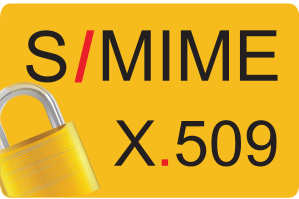
\includegraphics[width=1.5cm]{images-compendium/smime-icon}}}
\newcommand{\IncludeImage}[2][]{
\begin{center}
\texorhtml{%
  \includegraphics[#1]{images-compendium/#2}%
}{%
  \htmlimg{../images-compendium/#2.png}%
}
\end{center}
}

% custom colors
\definecolor{gray}{rgb}{0.4,0.4,0.4}
\definecolor{lightgray}{rgb}{0.7,0.7,0.7}

\T\parindent 0cm
\T\parskip\medskipamount

% Get the version information from another file.
% That file is created by the configure script.
\input{version.tex}


% Define universal url command.
% Used for latex _and_ hyperlatex (redefine see below).
% 1. parameter = link text (optional);
% 2. parameter = url
% e.g.: \uniurl[example link]{http:\\example.com}
\newcommand{\uniurl}[2][]{%
\ifthenelse{\equal{#1}{}}
{\texorhtml{\href{#2}{\Filename{#2}}}{\xlink{#2}{#2}}}
{\texorhtml{\href{#2}{\Filename{#1}}}{\xlink{#1}{#2}}}}

%%% HYPERLATEX %%%
\begin{ifhtml}
    % HTML title
    \htmltitle{Gpg4win Compendium}
    % TOC link in panel
    \htmlpanelfield{Contents}{hlxcontents}
    % link to DE version
    \htmlpanelfield{\htmlattributes*{img}{style=border:none title=German}
        \htmlimg{../images-hyperlatex/german.png}{German}}{../de/\HlxThisUrl}
    % name of the html files
    \htmlname{gpg4win-compendium}
    % redefine bmod
    \newcommand{\bmod}{mod}
    % use hlx icons (default path)
    \newcommand{\HlxIcons}{../images-hyperlatex}

    % Footer
    \htmladdress{$\copyright$ \compendiumDateEN, v\compendiumVersionEN
        %\manualinprogress
    \html{br/}
    \html{small}
    The Gpg4win Compendium is filed under the
    \link{GNU Free Documentation License v1.2}{fdl}.
    \html{/small}}

    % Changing the formatting of footnotes
    \renewenvironment{thefootnotes}{\chapter*{Fu�noten}\begin{description}}{\end{description}}

    % redefine universal url for hyperlatex (details see above)
    \newcommand{\linktext}{0}
    \renewcommand{\uniurl}[2][]{%
        \renewcommand{\linktext}{1}%
        % link text is not set
        \begin{ifequal}{#1}{}%
            \xlink{#2}{#2}%
            \renewcommand{linktext}{0}%
        \end{ifequal}
        % link text is set
        \begin{ifset}{linktext}%
             \xlink{#1}{#2}%
    \end{ifset}}


    % SECTIONING:
    %
    % on _startpage_: show short(!) toc (only part+chapter)
    \setcounter {htmlautomenu}{1}
    % chapters should be <H1>, Sections <H2> etc.
    % (see hyperlatex package book.hlx)
    \setcounter{HlxSecNumBase}{-1}
    % show _numbers_ of parts, chapters and sections in toc
    \setcounter {secnumdepth}{1}
    % show parts, chapters and sections in toc (no subsections, etc.)
    \setcounter {tocdepth}{2}
    % show every chapter (with its sections) in _one_ html file
    \setcounter{htmldepth}{2}

    % set counters and numberstyles
    \newcounter{part}
    \renewcommand{\thepart}{\arabic{part}}
    \newcounter{chapter}
    \renewcommand{\thecapter}{\arabic{chapter}}
    \newcounter{section}[chapter]
    \renewcommand{\thesection}{\thechapter.\arabic{section}}
\end{ifhtml}


%%% TITLEPAGE %%%

\title{
    \htmlattributes*{img}{width=300}
    \IncludeImage[width=0.5\textwidth]{gpg4win-logo}%
    \T~\newline
    \T\ifthenelse{\boolean{DIN-A5}}%
    % DIN A5:
    {\begin{latexonly}
        \LARGE The Gpg4win Compendium\\[0.3cm]
        \large \textmd{Secure e-mail and file encryption
        \\[-0.3cm] using GnuPG for Windows}
     \end{latexonly}  
    }%
    % DIN A4:
    {The Gpg4win Compendium \\
      \texorhtml{\Large \textmd}{\large}
      {Secure e-mail and file encryption using GnuPG for 
      Windows}
    }
}
\author{
    % Hyperlatex: Add links to pdf versions and Homepage
    \htmlonly{
        \xml{p}\small
        \xlink{Current PDF version as a
        download}{http://wald.intevation.org/frs/?group_id=11}\xml{br}
        To the \xlink{Gpg4win homepage}{http://www.gpg4win.org/}\xml{p}
    }
    % Authors
    \T\\[-1cm]
      \small Based on a version by
    \T\\[-0.2cm]
      \small Ute Bahn, Karl Bihlmeier, Manfred J. Heinze,
      \small Isabel Kramer und Dr. Francis Wray.
      \texorhtml{\\[0.2cm]}{\\}
      \small Extensively revised by
    \T\\[-0.2cm]
      \small Werner Koch, Florian v. Samson, Emanuel Sch�tze and Dr. Jan-Oliver Wagner.
      \texorhtml{\\[0.2cm]}{\\}
      \small Translated from the German original by
    \T\\[-0.2cm]
      \small Brigitte Hamilton
    \T\\[0.4cm]
}

\date{
    \T\ifthenelse{\boolean{DIN-A5}}%
    % DIN A5:
    {\begin{latexonly}
        \large A publication of the Gpg4win Initiative
        \\[0.2cm]
        Version \compendiumVersionEN~from \compendiumDateEN 
     \end{latexonly}
    }%
    % DIN A4:
    {A publication of the Gpg4win Initiative
      \\[0.2cm]
      Version \compendiumVersionEN~from \compendiumDateEN 
    }
}


% BEGIN DOCUMENT %%%

\begin{document}
\T\pdfbookmark[0]{Title page}{titel}
% set title page
\texorhtml{
    \ifthenelse{\boolean{DIN-A5}}
    {\noindent\hspace*{7mm}\parbox{\textwidth}{\centering\maketitle}\cleardoublepage}
    {\maketitle}
}
{\maketitle}


% improved handling of long (outstanding) lines
\T\setlength\emergencystretch{3em} \tolerance=1000


\T\section*{Publisher's details}
\W\chapter*{Publisher's details}\\

\thispagestyle{empty}
Copyright \copyright{} 2002 Bundesministerium f�r Wirtschaft und
Technologie\footnote{Any copying, distribution and/or modification to
this document may not create any impression of an association with the
Bundesministerium f�r Wirtschaft und Technologie 
(Federal Ministry for
Economics and Technology)}\\
Copyright \copyright{} 2005 g10 Code GmbH\\
Copyright \copyright{} 2009, 2010 Intevation GmbH

Permission is granted to copy, distribute and/or modify this document
under the terms of the GNU Free Documentation License, Version 1.2 or
any later version published by the Free Software Foundation; with no
Invariant Sections, no Front-Cover Texts, and no Back-Cover Texts. A
copy of the license is included in the section entitled ``GNU Free
Documentation License''.



\clearpage
\chapter*{About this compendium}
\T\ifthenelse{\boolean{DIN-A5}}{\enlargethispage{2\baselineskip}}{}

The Gpg4win Compendium consists of three parts:

\begin{itemize}
\item \textbf{Part~\link*{1}[\ref{part:Novices}]{part:Novices}
    ``For Novices''}: A quick course in Gpg4win.

\item \textbf{Part~\link*{2}[\ref{part:AdvancedUsers}]{part:AdvancedUsers} 
    ``For Advanced Users''}: Background information for Gpg4win.

\item \textbf{Annex}: Additional technical information about Gpg4win.\\
\end{itemize}

\textbf{Part~\link*{1}[\ref{part:Novices}]{part:Novices} ``For
Novices''} provides a brief guide for the installation and daily use
of Gpg4win program components.  The practice robot \textbf{Adele}
will help you with this process and allow you to practice
the de- and encryption process (using OpenPGP) until you 
have become familiar with Gpg4win.

The amount of time required to work through this brief guide will
depend on your knowledge of your computer and Windows.
It should take about one hour.\\

\textbf{Part~\link*{2}[\ref{part:AdvancedUsers}]{part:AdvancedUsers}
``For Advanced Users''} provides background information which
illustrates the basic mechanisms on which Gpg4win is based, and also
explains some of its less commonly used capabilities.  Part I and II can be
used independently of each other. However, to achieve an optimum
understanding, you should read both parts in the indicated sequence,
if possible.\\

The \textbf{Annex} contains details regarding the specific technical
issues surrounding Gpg4win, including the GpgOL Outlook program
extension.\\

Just like the cryptography program package Gpg4win, this compendium was
not written for mathematicians, secret service agents or
cryptographers, but rather was written to be read and
understood \textbf{by anyone.}\\

The Gpg4win program package and compendium can be obtained at: \\
\uniurl{http://www.gpg4win.org}

\clearpage
\chapter*{Legend\htmlonly{\html{br}\html{br}}}

This compendium uses the following text markers:
\begin{itemize} 
    \item \textit{Italics} are used for text that appears on a screen
        (e.g. in menus or dialogs). In addition, square
        brackets are used to mark \Button{buttons}. 

        Sometimes italics will also be used for individual words in
        the text, if their meaning in a sentence is to be highlighted
        without disrupting the text flow, by using \textbf{bold} fond
        (e.g.\textit{only } OpenPGP).

    \item \textbf{Bold} is used for individual words or sentences
        which are deemed particularly important and hence must be
        highlighted. These characteristics make it easier for readers
        to quickly pick up highlighted key terms and important
        phrases.

    \item \texttt{Typewriter font} is used for all file names, paths,
        URLs, source codes, as well as inputs and outputs (e.g. for
        command lines).  
\end{itemize}

\cleardoublepage
\T\pdfbookmark[0]{\contentsname}{toc}
\tableofcontents

%%%%%%%%%%%%%%%%%%%%%%%%%%%%%%%%%%%%%%%%%%%%%%%%%%%
% Part I
\clearpage
\T\part{For Novices}
\W\part*{\textbf{I For Novices}}
\label{part:Novices}
\addtocontents{toc}{\protect\vspace{0.3cm}}
\addtocontents{toc}{\protect\vspace{0.3cm}}


\chapter{Gpg4win -- Cryptography for Everyone}
\index{Cryptography}

What is Gpg4win? Wikipedia answers this question as follows:

\begin{quote}
    \textit{Gpg4win is an installation package for Windows
    (2000/XP/2003/Vista) with computer programs and
    handbooks for \Email{}and file encryption. It includes the
    GnuPG encryption software, as well as several applications and
    documentation. Gpg4win itself and the programs contained in
    Gpg4win are Free Software.}
\end{quote}

The ``Novices'' and ``Advanced Users'' handbooks have been combined for
this second version under the name ``Compendium''. In Version 2,
Gpg4win includes the following programs:

\begin{itemize}
    \item \textbf{GnuPG}\index{GnuPG}\\ GnuPG forms the heart of
        Gpg4win -- the actual encryption software.
    \item \textbf{Kleopatra}\index{Kleopatra}\\ The central
        certificate administration\index{Certificate Administration} of
        Gpg4win, which ensures uniform user navigation for all
        cryptographic operations.
    \item \textbf{GNU Privacy Assistant (GPA)}\index{GNU Privacy
        Assistent|see{GPA}}\index{GPA}\\ is an alternative program for
        managing certificates, in addition to Kleopatra.
    \item \textbf{GnuPG for Outlook (GpgOL)}\index{GnuPG f�r
        Outlook|see{GpgOL}}\index{GpgOL}\\ is an extension for
        Microsoft Outlook 2003 and 2007, which is used to sign and
        encrypt messages.
   \item \textbf{GPG Explorer eXtension (GpgEX)}\index{GPG Explorer
       eXtension|see{GpgEX}}\index{GpgEX}\\ is an extension for
       Windows Explorer\index{Windows-Explorer} which can be used to
       sign and encrypt files using the context menu.
    \item \textbf{Claws Mail}\index{Claws Mail}\\ is a
        full \Email{} program that offers very good support for GnuPG.
\end{itemize}

Using the GnuPG (GNU Privacy Guard) encryption program,
anyone can encrypt \Email{}s securely, easily and at no cost. GnuPG can be
used privately or commercially without any restrictions. The
encryption technology used by GnuPG is secure, and cannot be broken
based on today's state of technology and research.

GnuPG is \textbf{Free Software}\footnote{Often also referred to as
Open Source Software (OSS).}.\index{Free Software} That means that
each person has the right to use this software for private or
commercial use. Each person may and can study the source code of the
programs and -- if they have the required technical knowledge -- make
modifications and forward these to others.

With regard to security software, this level of transparency --
guaranteed access to the source code -- forms an indispensable
foundation. It is the only way of actually checking the
trustworthiness of the programming and the program itself.

GnuPG is based on the international standard
\textbf{OpenPGP}\index{OpenPGP} (RFC 2440), which is fully compatible with
PGP and also uses the same infrastructure (certificate server etc.) as the
latter. Since Version 2 of GnuPG, the cryptographic
standard\textbf{S/MIME}\index{S/MIME} (IETF RFC 3851, ITU-T
X.509\index{X.509} and ISIS-MTT/Common PKI) are also supported.

PGP (``Pretty Good Privacy'')\index{PGP} is not Free Software; many
years ago, it was briefly available at the same conditions as GnuPG.
However, this version has not corresponded with the latest state of
technology for some time.

Gpg4win's predecessors were supported by the Bundesministerium f�r
Wirtschaft und Technologie \index{Bundesministerium f�r Wirtschaft und
Technologie} as part of the Security on the Internet initiative.
Gpg4win and Gpg4win2 were supported by the Bundesamt f�r Sicherheit in
der Informationstechnik (BSI). \index{Bundesamt f�r Sicherheit in der
Informationstechnik}


Additional information on GnuPG and other projects undertaken by the Federal Government for security on the Internet can be found on the webpages
\uniurl[www.bsi.de]{http://www.bsi.de} and 
\uniurl[www.bsi-fuer-buerger.de]{http://www.bsi-fuer-buerger.de} of the Bundesamt f�r Sicherheit in der Informationstechnik.


\clearpage
\chapter{Encrypting \Email{}s: because the envelope is missing}
\label{ch:why}
\index{Envelope}

The encryption of messages is sometimes described as the second-oldest
profession in the world. Encryption techniques were used as far back
as Egypt's pharaoh Khnumhotep II, and during Herodot's and Cesar's time. Thanks
to Gpg4win, encryption is no longer the reserve of kings, but is
accessible to everyone, for free.

\htmlattributes*{img}{width=300}
\IncludeImage[width=0.9\textwidth]{egyptian-stone}

Computer technology has provided us with some excellent tools to
communicate around the globe and obtain information. However, rights
and freedoms which are taken for granted with other forms of
communication must still be secured when it comes to new technologies.
The Internet has developed with such speed and at such a scale that it
has been difficult to keep up with maintaining our rights. 

With the old-fashioned way of writing a letter, written contents are
protected by an envelope. The envelope protects messages from prying
eyes, and it is easy to see if an envelope has been manipulated. Only
if the information is not important, do we write it on an unprotected
post card, which can also be read by the mail carrier and others.

\clearpage
You and no one else decides whether the message is important,
confidential or secret. 

\Email{}s do not provide this kind of freedom. An \Email{} is like a
post card - always open, and always accessible to the electronic
mailman and others. It gets even worse: while computer technology
offers the option of transporting and distributing millions of
\Email{}s, it also provides people with the option of checking them.

Previously, no one would have seriously thought about collecting all
letters and postcards, analyse their contents or monitor senders and
recipients. It would not only have been unfeasiable, it would have
also taken too long. However, modern computer technology has made this
a technical possibility. There are indications that this is already
being done on a large scale. A Wikipedia article on the Echelon
system\footnote{\uniurl[\EchelonUrl]{\EchelonUrl}} \index{Echelon
system} provides interesting background information on this topic.

Why is this an issue -- because the envelope is missing.

\htmlattributes*{img}{width=300}
\IncludeImage[width=0.5\textwidth]{sealed-envelope}

\clearpage
What we are suggesting here is essentially an ``envelope'' for your
electronic mail. Whether you use it, when or for whom and how often -
that is entirely up to you. Software such as Gpg4win merely returns 
the right to choose to you.  The right to choose whether you think a message
is important and requires protection. 

This is the key aspect of the right to privacy of correspondence, post
and telecommunications in \index{Telecommunication secrecy}
\index{Mail secrecy}\index{Correspondence secrecy} the Basic Law, and
the Gpg4win program package allows you to exercise this right. You do
not have to use this software, just as you are not required to use an
envelope.  But you have the right.

To secure this right, Gpg4win offers a so-called ``strong encryption
technology''.  ``Strong'' in this sense means that it cannot be broken
with known tools. Until recently, strong encryption methods used to be
reserved for military and government circles in many countries. The
right to make them accessible to all citizens was championed by
Internet users, and sometimes also with the help of visionary people
in government institutions, as was the case with support for Free
Software for encryption purposes. Security experts around the world
now view GnuPG as a practical and secure software.

\textbf{It is up to you how you want to value this type of security.}

You alone decide the relationship between the convenience of encryption
and the highest possible level of security. These include the few but
important precautions you must make to implement to ensure that
Gpg4win can be used properly. This compendium will explain this
process on a step-by-step basis.


\clearpage
\chapter{How Gpg4win works}
\label{ch:FunctionOfGpg4win}
The special feature of Gpg4win and its underlying
\textbf{``Public Key'' method}\index{public key method@``Public Key'' Method}
is that anyone can and should understand it. There is nothing
secretive about it -- it is not even very difficult to understand.

The use of individual Gpg4win program components is very simple, even
though the way it works is actually quite complicated. This section
will explain how Gpg4win works -- not in all details, but enough to
explain the principles behind this software. Once you are familiar
with the principles, you will have considerable trust in the security
offered by Gpg4win. 

At the end of this book, in Chapter~\ref{ch:themath}, you can also open
the remaining secrets surrounding ``Public Key'' cryptography and
discover why it is not possible to break messages encrypted with
Gpg4win using current state of technology.

\clearpage
\subsubsection{Lord of the keyrings}
Anyone wishing to secure something valuable locks it away -- with a
key. Even better is a key that is unique and is kept in a safe
location. 

\htmlattributes*{img}{width=300}
\IncludeImage[width=0.5\textwidth]{schlapphut-with-key}

If the key should ever fall into the wrong hands, the valuables are no
longer secure. Their security stands and falls with the security and
uniqueness of the key. Therefore the key must be at least as well
protected as the valuables themselves. To ensure that it cannot be
copied, the exact characteristics of the key must also be kept secret.

\clearpage
Secret keys are nothing new in cryptography: it has always been that
keys were hidden to protect the secrecy of the messages. Making this
process very secure is very cumbersome and also prone to errors.

\htmlattributes*{img}{width=300}
\IncludeImage[width=0.5\textwidth]{tangled-schlapphut}

The basic problem with the ``ordinary'' secret transmission of messages
is that the same key is used for both encryption and decryption, and
that both the sender as well as recipient must be familiar with this
secret key. For this reason, these types of encryption systems are
also called \textbf{``symmetric encryption''}.\index{Symmetric encryption}

This results in a fairly paradoxical situation: Before we can use this
method to communicate a secret (an encrypted message), we must have
also communicated another secret in advance: the key. And that is
exactly the problem, namely the constantly occuring issue of
always having to exchange keys while ensuring that they are not
intercepted by third parties.


\clearpage
In contrast -- and not including the secret key -- Gpg4win works with
another key that is fully accessible and public. It is also described
as a ``public key'' encryption system. 

This may sound contradictory, but it is not. The clue: It is no longer
necessary to exchange a secret key. To the contrary: The secret key
can never be exchanged! The only key that can be passed on is the
public key (in the public certificate)~-- which anyone can know. 

That means that when you use Gpg4win, you are actually using a pair of
keys\index{Key!pair} -- a secret and a second public key. Both key
components are inextricably connected with a complex mathematical
formula. Based on current scientific and technical knowledge, it is
not possible to calculate one key component using the other, and it is
therefore impossible to break the method. 

Section \ref{ch:themath} explains why that is.

\htmlattributes*{img}{width=300}
\IncludeImage[width=0.5\textwidth]{verleihnix}


\clearpage
The principle behind public key encryption\index{public key method@``Public Key'' Method}

The \textbf{secret} or \textbf{private key} must be kept secret.

The \textbf{public key} should be as accessible to the general public as much as
possible.

Both key components have very different functions:

\bigskip

\begin{quote}
    The secret key component \textbf{decrypts} messages.
\end{quote}

\htmlattributes*{img}{width=300}
\IncludeImage[width=0.75\textwidth]{key-with-shadow-bit}

\begin{quote}
    The public key component \textbf{encrypts} messages.
\end{quote}


\clearpage
\subsubsection{The public mail strongbox}
\index{Mail strongbox}

This small exercise is used to explain the difference between the
``public key'' encryption system and symmetric
encryption\index{Symmetric encryption} (``non-public key''
method)
\index{non-public key mehtod@``Non-Public Key'' Method|see{Symmetric encryption}} ...

\bigskip

\textbf{The ``secret key method'' works like this:}

Imagine that you have installed a mail strongbox in front of your
house, which you want to use to send secret messages. 

The strongbox has a lock for which there is only one single key. No
one can put anything into or take it out of the box without this key.
This way, your secret messages are pretty secure.

\htmlattributes*{img}{width=300}
\IncludeImage[width=0.75\textwidth]{letter-into-safe}

Since there is only one key, the person you are corresponding with
must have the same key that you have in order to open and lock the mail
strongbox, and to deposit a secret message.

\clearpage
You have to give this key to that person via a secret route.

\bigskip
\bigskip

\htmlattributes*{img}{width=300}
\IncludeImage[width=0.75\textwidth]{secret-key-exchange}

\clearpage
They can only open the strongbox and read the secret message once they
have the secret key.

Therefore everything hinges on this one key: If a third party knows
the key, it is the end of the secret messages.  Therefore you and the
person you are corresponding with \textbf{must exchange the key in a
manner that is as secret} as the message itself. 

But actually -- you might just as well give them the secret message
when you are giving them the key...

\textbf{How this applies to \Email{} encryption:} Around the world,
all participants would have to have secret keys and exchange
these keys in secret before they can send secret messages
per \Email{}.

So we might as well forget about this option ...

\htmlattributes*{img}{width=300}
\IncludeImage[width=0.75\textwidth]{letter-out-of-safe}

\clearpage
\textbf{Now the ``public key'' method}

You once again install a mail strongbox\index{Mail strongbox} in front of
your house. But unlike the strongbox in the first example, this one
is always open. On the box hangs a key --� which is visible to
everyone -- and which can be used by anyone to lock the strongbox
(asymetric encryption method).
\index{Asymmetric encryption}

\textbf{Locking, but not opening:} that is the difference!

\htmlattributes*{img}{width=300}
\IncludeImage[width=0.7\textwidth]{pk-safe-open}

This key is yours and -- as you might have guessed -- it is your public key.

If someone wants to leave you a secret message, they put it in the
strongbox and lock it with your public key. Anyone can do this, since
the key is available to everyone.  

No one else can open the strongbox
and read the message.  Even the person that has locked the message in
the strongbox cannot unlock it again, e.g. in order to change the
message.  

This is because the public half of the key can only be used for locking purposes.

The strongbox can only be opened with one single key: your own secret
and private part of the key.

\clearpage
\textbf{Getting back to how this applies to \Email{} encryption:}
Anyone can encrypt an \Email{} for you.  

To do this, they do not need a secret key; quite the opposite, they
only need a totally non-secret \index{Key!public}, ``public'' key.
Only one key can be used to decrypt the \Email{}, namely your private
and secret key\index{Key!private}.

You can also play this scenario another way:

If you want to send someone a secret message, you use their mail
strongbox with their own public and freely available key.

To do this, you do not need to personally know the person you are
writing to, or have to speak to them, because their public key is
always accessible, everywhere. One you have placed your message in the
strongbox and locked it with the recipient's key, the message is not
accessible to anyone, including you. Only the recipient can open the
strongbox with his private key and read the message.

\T\enlargethispage{2\baselineskip}

\htmlattributes*{img}{width=300}
\IncludeImage[width=0.75\textwidth]{pk-safe-opened-with-sk}

\clearpage
\textbf{But what did we really gain:} There is still a secret
key!



However, this is quite different from the ``non-public key'' method:
You are the only one who knows and uses your secret key. The key is
never forwarded to a third party  �-- it is not necessary to transfer
keys in secret, nor is it advised.

Nothing must be passed between sender and recipient in secret --
whether a secret agreement or a secret code.

And that is exactly the crux of the matter: All symmetric encryption
methods can be broken because a third party has the opportunity to
obtain the key while the key is being exchanged.

This risk does not apply here, because there is no exchange of secret
keys; rather, it can only be found in one and very secure location:
your own keyring\index{Key!pair} -- your own memory.

This modern encryption method which uses a non-secret and public key,
as well as a secret and private key part is also described as
``asymmetric encryption''. \index{Asymmetric encryption}


\clearpage
\chapter{The passphrase}
\label{ch:passphrase}
\index{Passphrase}

As we have seen in the last chapter, the private key is one of the
most important components of the ``public key'' or asymmetric
encryption method. While one no longer needs to exchange the key with
another party in secret, the security of this key is nevertheless the
"key"  to the security of the ``entire'' encryption process.

On a technical level, a private key is nothing more than a file which
is stored on your computer. To prevent unauthorised access of this
file, it is secured in two ways:

\htmlattributes*{img}{width=300}
\IncludeImage[width=0.5\textwidth]{think-passphrase}

First, no other user may read or write in the file -- which is
difficult to warrant, since computer administrators always have access
to all files, and the computer may be lost or attacked 
by viruses\index{Viruses}, worms\index{Worms} or
Trojans\index{Trojans} .

For this reason we need another layer of protection: the passphrase.
This is not a password -- a passphrase should not consist of only one
word, but a sentence, for example. You really should keep this
passphrase ``in your head'' and never have to write it down.  

At the same time, it cannot be possible to guess it.  This may sound
contradictory, but it is not. There are several proven methods of
finding very unique and easy to remember passphrases, which cannot be
easily guessed.

\clearpage
Think of a phrase that is very familiar to you, e.g.:

$\qquad$\verb-People in glass houses should not be throwing stones.-

Now, take every third letter of this sentence:

$\qquad$\verb-oegsoehloerisn- 
\texttt{\scriptsize{(Pe\textbf{o}pl\textbf{e} in
\textbf{g}la\textbf{s}s h\textbf{o}us\textbf{e}s
s\textbf{h}ou\textbf{l}d n\textbf{o}t b\textbf{e}
th\textbf{r}ow\textbf{i}ng \textbf{s}to\textbf{n}es.)}} 


While it may not be easy to remember
this sequence of letters, it is also unlikely that you will forget how
to arrive at the passphrase it as long as you remember the original
sentence. Over time, and the more often you use the phrase, you will
commit it to memory. No one else can guess the passphrase.

Think of an event that you know you will never forget about. Maybe
it's a phrase that you will always associate with your child or
partner, i.e. it has become ``unforgettable''.  Or a holiday memory or
a line of text of a song that is personally important to you.

Use capital and small letters, numbers, special characters and spaces,
in any order. In principle, anything goes, including umlaute, special
characters, digits etc. But remember -- if you want to use your secret
key abroad at a different computer, please remember that not all
keyboards may have such special characters. For example, you will
likely only find umlaute (�, �, � usw.) on German keyboards.  

You can also make intentional grammar mistakes, e.g.  ``mustake''
instead of ``mistake''. Of course you also have to be able to remember
these ``mustakes''. Or, change languages in the middle of the phrase.
You can change the sentence:

$\qquad$\verb-In M�nchen steht ein Hofbr�uhaus.-

into this passphrase:

$\qquad$\verb-inMinschen stet 1h0f breuhome-

Think of a sentence that does not make sense, but you can still remember
e.g.:

$\qquad$\verb-The expert lamenting nuclear homes-

$\qquad$\verb-Knitting an accordeon, even during storms.-

A passphrase of this length provides good protection for your
secret key.

It can also be shorter if you use capital letters,
for example:

$\qquad$\verb-THe ExPERt laMenTIng NuclEAr hoMES.-

While the passphrase is now shorter, it is also more difficult to
remember. If you make your passphrase even shorter by using special
characters, you will save some time entering the passphrase, but it is
also morr likely that you will forget your passphrase.

Here is an extreme example of a very short but also very secure 
passphrase:

$\qquad$\verb-R!Qw"s,UIb *7\$-

However, in practice, such sequences of characters have not proven
themselves to be very useful, since there are simply too few clues by
which to remember them.


\clearpage
A \textbf{bad passphrase} can be ``broken'' very quickly, if it ...

\begin{itemize}
    \item ... is already used for another purpose (e.g. for an \Email{} account or your mobile phone). The
        same passphrase would therefore already be known to another,
        possibly not secure, software. If the hacker is successful,
        your passphrase becomes virtually worthless.

    \item ... comes from a dictionary. Passphrase finder programs can
        run a password through complete digital dictionaries in a
        matter of minutes -- until it matches one of the words.

    \item ... consists of a birth date, a name or other public
        information. Anyone planning to decrypt your
       \Email{} will obtain this type of
        information.

    \item ... is a very common quote, such as ``to be or not to be''.
        Passphrase finder programs also use quotes like these to break
        passphrases.

    \item ... consists of only one word or less than 8 characters. It
        is very important that you think of a longer passphrase.
\end{itemize}

When composing your passphrase, please \textbf{do not use} any of the
aforementioned examples. Because anyone seriously interested in
getting his hands on your passphrase will naturally see if you used
one of these examples.

\bigskip

\textbf{Be creative!} Think of a passphrase now! Unforgettable and unbreakable.

In Chapter~\ref{ch:CreateKeyPair} you will need this passphrase to create your key pair.

But until then, you have to address another problem: Someone has to
verify that the person that wants to send you a secret message is
real.


\clearpage
\chapter{Two methods, one goal: OpenPGP \& S/MIME}
\label{ch:openpgpsmime}
\index{OpenPGP} \index{S/MIME}

You have seen the importance of the ``envelope'' for your
\Email{} and how to provide one 
using tools of modern information technology: a mail
strongbox,\index{Mail strongbox} in which anyone can deposit encrypted
mails which only you, the owner of the strongbox, can decrypt. It is
not possible to break the encryption as long as the private key to
your ``strongbox'' remains your secret.

Still: If you think about it, there is still another problem. A little
further up you read about how -- in contrast to the secret key method
-- you do not need to personally meet the person you are corresponding
with in order to enable them to send a secret message. But how can you
be sure that this person is actually who they say they
are? In the case of \Email{}s, you
only rarely know all of the people you are corresponding with on a
personal level -- and it is not usually easy to find out who is really
behind an \Email{} address. Hence, we not only
need to warrant the secrecy of the message, but also the identity of
the sender -- specifically \textbf{authenticity}. \index{Authenticity}

Hence someone must authenticate that the person who wants to send you
a secret message is real. In everyday life, we use ID, signatures or
certificates authenticated by authorities or notaries for
\index{Authentication} ``authentication'' purposes. These
institutions derive their right to issue notarisations from a
higher-ranking authority and finally from legislators. Seen another
way, it describes a chain of trust which
runs \index{Chain of trust} from ``the top'' to ``the bottom'', and is
described as a \textbf{``hierarchical trust concept''}.
\index{Hierarchical trust concept}

In the case of Gpg4win or other \Email{} encryption programs, 
 this concept is found in almost mirror-like fashion in
\textbf{S/MIME}. Added to this is\textbf{OpenPGP}, another concept
that only works this way on the Internet.  S/MIME und OpenPGP have the
same task: the encryption and signing of data.  Both use the already
familiar public key method.  While there are some important
differences, in the end, none of these standards offer any general
advantage over another. For this reason you can use Gpg4win to use
both methods.


\clearpage
The equivalent of the hierarchical trust concept is called ``Secure /
Multipurpose Internet Mail Extension'' or \textbf{S/MIME}. If you use
S/MIME, your key must be authenticated by an accredited
organisation before it can be used. The certificate of this
organisation in turn was authenticated by a higher-ranking
organisation etc. -- until we arrive at a so-called root certificate.
This hierarchical chain of trust usually has three links: the root
certificate, the certificate of the issuer of the
certificate\index{Certificate issuer} (also CA\index{Certificate
Authority (CA)} for Certificate Authority), and finally your own user
certificate.

A second alternative and non-compatible notarisation method is the
\textbf{OpenPGP} standard, does not build a trust hierarchy but rather
assembles a \textbf{``Web of trust''}.\index{Web of Trust}
The Web of Trust represents the basic structure of the
non-hierarchical Internet and its users. For example, if User B trusts
User A, then User B could also trust the public key of User C, whom he
does not know, if this key has been authenticated by User A.

Therefore OpenPGP offers the option of exchanging encrypted data and 
\Email{}s without authentication by a higher-ranking agency. It is
sufficient if you trust the \Email{} address and
associated certificate of the person you are communicating with.

Whether with a trust hierarchy or Web of Trust -- the authentication
of the sender is at least as important as protecting the message. We
will return to this important protection feature later in the
compendium. For now, this information should be sufficient to install
Gpg4win and understand the following chapters:

\begin{itemize}
    \item Both methods -- \textbf{OpenPGP} and\textbf{S/MIME} --
        offer the required security.
    \item The methods are \textbf{not compatible} with each other.
        They offer two alternate methods for authenticating your
        secret communication. Therefore they are not deemed to be 
        interoperable.
    \item Gpg4win allows for the convenient \textbf{and parallel} use
        of both methods -- you do not have to choose one or the other
        for encryption/signing purposes.
\end{itemize}

Chapter~\ref{ch:CreateKeyPair} of this compendium, which discusses the
creation of the key pair, therefore branches off to discuss both methods. At
the end of Chapter~\ref{ch:CreateKeyPair} the information is combined
again.

\begin{latexonly} %no hyperlatex
In this compendium, these two symbols will be used to refer to the two
alternative methods:

\begin{center}

\includegraphics[width=2.5cm]{images-compendium/openpgp-icon}
\hspace{1cm}
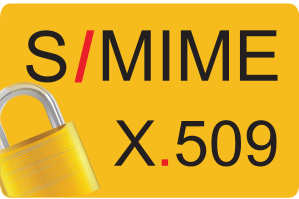
\includegraphics[width=2.5cm]{images-compendium/smime-icon}
\end{center}
\end{latexonly}


\clearpage
\chapter{Installing Gpg4win}
\index{Installation}

Chapters 1 to 5 provided you with information on the background
related to encryption. While Gpg4win also works if you do not
understand the logic behind it, it is also different from other
programs in that you are entrusting your secret correspondence to this
program. Therefore it is good to know how it works.  

With this knowledge you are now ready to install Gpg4win and set up
your key pair.

If you already have a GnuPG-based application installed on your
computer (e.g. GnuPP, GnuPT, WinPT or GnuPG Basics), please refer to
the Annex~\ref{ch:migration} for information on transferring your
existing certificates.

You can load and install Gpg4win from the Internet or a CD. To do
this, you will need administrator rights to your Windows operating
system. 

If you are downloading Gpg4win from the Internet, please ensure that
you obtain the file from a trustworthy site, e.g.:
\uniurl[www.gpg4win.org]{http://www.gpg4win.org}. To start the
installation, click on the following file after the download:

\Filename{gpg4win-2.0.0.exe} (or higher version number).

If you received Gpg4win on a CD ROM, please open it and click on the
``Gpg4win'' installation icon.  All other installation steps are the
same.

The response to the question of whether you want to install the
program is \Button{Yes}.

\clearpage
The installation assistant will start and ask you for the language to
be used with the installation process:

% screenshot: Installer Sprachenauswahl
\IncludeImage[width=0.5\textwidth]{sc-inst-language_en}

Confirm your language selection with \Button{OK}.

Afterwards you will see this welcome dialog:

% screenshot: Installer Willkommensseite
\IncludeImage[width=0.85\textwidth]{sc-inst-welcome_en}

Close all programs that are running on your computer and click
on \Button{Next}.

\clearpage
The next page displays the \textbf{licensing agreement} -- it is only
important if you wish to modify or forward Gpg4win.  If you only want
to use the software, you can do this right away -- without reading the
license.

% screenshot: Lizenzseite des Installers
\IncludeImage[width=0.85\textwidth]{sc-inst-license_en}

Click on \Button{Next}.

\clearpage
On the page that contains \textbf{the selection of components} you can
decide which programs you want to install.

A default selection has already been made for you. Yo can also insall
individual components at a later time. 

Moving your mouse cursor over a component will display a brief
description.  Another useful feature is the display of required hard
drive space for all selected components.

% screenshot: Auswahl zu installierender Komponenten
\IncludeImage[width=0.85\textwidth]{sc-inst-components_en}

Click on \Button{Next}.

\clearpage
The system will suggest a folder for the installation, e.g.:
\Filename{C:$\backslash$Programme$\backslash$GNU$\backslash$GnuPG}

You can accept the suggestion or select a different folder for installing
Gpg4win.

% screenshot: Auswahl des Installationsverzeichnis.
\IncludeImage[width=0.85\textwidth]{sc-inst-directory_en}

Then click on \Button{Next}.

\clearpage
Now you can decide which \textbf{links} should be insalled -- the
system will automatically create a link with the start menu. You can
change this link later on using the Windows dashboard settings.

% screenshot: Auswahl der Startlinks
\IncludeImage[width=0.85\textwidth]{sc-inst-options_en}

Then click on \Button{Next}.

\clearpage
If you have selected the default setting -- \textbf{link with start
menu} -- you can define the name of this start menu on the next page
or simply accept the name. 

% screenshot:  Startmenu ausw�hlen
\IncludeImage[width=0.85\textwidth]{sc-inst-startmenu_en}

Then click on \Button{Install}.

\clearpage
During the \textbf{installation} process that follows, you will see a progress bar and information on which file is currently being installed. You can press \Button{Show~details}
at any time to show the installation log.

% screenshot: Ready page Installer
\IncludeImage[width=0.85\textwidth]{sc-inst-progress_en}

Once you have completed the installation, please click on
\Button{Next}.

\clearpage
The last page of the installation process is shown once the
installation has been successfully completed:

% screenshot: Finish page Installer
\IncludeImage[width=0.85\textwidth]{sc-inst-finished_en}

You have the option of displaying the README file, which contains
important information on the Gpg4win version you have just installed.
If you do not wish to view this file, deactivate this option.

Then click on \Button{Finish}.

\clearpage
In some cases you may have to restart Windows. In this case, you will
see the following page:

% screenshot: Finish page Installer with reboot
\IncludeImage[width=0.85\textwidth]{sc-inst-finished2_en}

Now you can decide whether Windows should be restarted immediately or
manually at a later time. 

Click on \Button{Finish}.

%TODO: NSIS-Installer anpassen, dass vor diesem
%Reboot-Installationsdialog auch ein Hinweis auf die README-Datei
%erscheint.
Please read the README file which contains up-to-date information on
the Gpg4win version that has just been installed. You can find this
file e.g. via the start menu:\\
\Menu{Start$\rightarrow$Programs$\rightarrow$Gpg4win$\rightarrow$Documentation$\rightarrow$Gpg4win README}

\clearpage
\textbf{And that's it!}

You have successfully installed Gpg4win and are ready to work with the
program.

For information on \textbf{automatically installing} Gpg4win, as may
be of interest for software distribution systems, please see the
Annex~\ref{ch:auto} ``Automatic installation of Gpg4win''.


\clearpage
\chapter{Creating a certificate}
\label{ch:CreateKeyPair}
\index{Certificate!create}
\index{Key!create}

Now that you have found out why GnuPG is so secure
(Chapter~\ref{ch:FunctionOfGpg4win}), and how a good passphrase
provides protection for your private key (Chapter~\ref{ch:passphrase}),
you are now ready to create your own key pair\index{Key!pair} .

As we saw in Chapter~\ref{ch:FunctionOfGpg4win}, a key pair consists of
a public and a private key.  With the addition of an
\Email{} address, login name etc., which you
enter when creating the pair (so-called meta data), you can obtain
your private certificate with the public \textit{and } private key.

This definition applies to both OpenPGP as well as S/MIME (S/MIME
certificates correspond with a standard described as
``X.509''\index{X.509}).

~\\ \textbf{It would be nice if I could practice this important
step of creating a key pair ....}

\T\marginOpenpgp
Not to worry, you can do just that -- but only with OpenPGP:

If you decide for the OpenPGP method of authentication,
\index{Authentication} the ``Web of Trust'', then you can practice the
entire process for creating a key pair, encryption and decryption as
often as you like, until you feel very comfortable.

This ``dry run'' will strengtthen your trust in Gpg4win, and the ``hot
phase'' of OpenPGP key pair creation will no longer be a problem for
you.

Your partner in this exercise is \textbf{Adele} . Adele is a test
service which is still derived from the GnuPP predecessor
project\index{GnuPP} and is still in operation. In this compendium we
continue to recommend the use of this practice robot. We would also
like to thank the owners of gnupp.de for operating this practice
robot.

Using Adele, you can practice and test the OpenPGP key pair
which you will be creating shortly, before you start using it in earnest.
But more on that later.

\clearpage
\textbf{Let's go!}
Open Kleopatra using the Windows start menu:

% screenshot Startmenu with Kleopatra highlighted
\htmlattributes*{img}{width=400}
\IncludeImage[width=0.7\textwidth]{sc-kleopatra-startmenu_en}

You will see the main Kleopatra screen\index{Kleopatra} --
the certificate administration:
\index{Certificate administration}

% screenshot: Kleopatra main window
\htmlattributes*{img}{width=508}
\IncludeImage[width=0.85\textwidth]{sc-kleopatra-mainwindow-empty_en}

At the beginning, this overview will be empty, since you have not
created or imported any certificates yet. 

\clearpage
Click on \Menu{File$\rightarrow$New~Certificate}. 

In the following dialog you select the format for the certificate. You
can choose from the following: \textbf{OpenPGP} (PGP/MIME)
or \textbf{X.509} (S/MIME).

The differences and common features of the two formats have already been
discussed in Chapter~\ref{ch:openpgpsmime}.

\label{chooseCertificateFormat}
% screenshot: Kleopatra - New certificate - Choose format
\IncludeImage[width=0.85\textwidth]{sc-kleopatra-ChooseCertificateFormat_en}

~\\ This chapter of the compendium breaks off into two
sections for each method at this point. Information is then combined
at the end of the Chapter.

Depending on whether you chose OpenPGP or X.509 (S/MIME), you can now
read either:
\begin{itemize}
    \item Section~\ref{createKeyPairOpenpgp}:
        \textbf{Creating an OpenPGP certificate} \T(siehe next
        page) or
    \item Section~\ref{createKeyPairX509}:
        \textbf{Creating an X.509 certificate} \T (see page
        \pageref{createKeyPairX509}).
\end{itemize}



\clearpage
\section{Creating an OpenPGP certificate}
\label{createKeyPairOpenpgp}
\index{OpenPGP!create certificate}

\T\marginOpenpgp
In the certificate option dialog, click on \Button{Create
personal OpenPGP key pair}.


Now enter your \Email{} address and your name in
the following window. Name and \Email{} address
will be made publicly visible later.

You also have the option of adding a comment for the key pair. Usually
this field stays empty, but if you are creating a key for test
purposes, you should enter "test" so you do not forget it is a test
key. This comment becomes part of your login name, and will become
public just like your name and \Email{} address.

% screenshot: Creating OpenPGP Certificate - Personal details
\IncludeImage[width=0.85\textwidth]{sc-kleopatra-openpgp-personalDetails_en}

If you first wish to \textbf{test} your OpenPGP key pair, you can
simply enter any name and fictional 
\Email{} address, e.g.:\\ \Filename{Heinrich Heine}
and \Filename{heinrich@gpg4win.de}

The \textbf{Advanced settings are only be required in exceptional}
cases. For details, see the Kleopatra handbook (via
\Menu{Help$\rightarrow$Kleopatra handbook}).

Click on \Button{Next}.

\clearpage You will see a list of all of the main entries and settings
for \textbf{review purposes}. If you are interested in the (default)
expert settings, you can view these via the \Menu{All details}
option.

% screenshot: Creating OpenPGP Certificate - Review Parameters
\IncludeImage[width=0.85\textwidth]{sc-kleopatra-openpgp-reviewParameters_en}

If everything is correct, click on \Button{Create key}.

\clearpage Now to the most important part: entering your
\textbf{passphrase}!

To create a key pair, you must enter your personal passphrase:

% screenshot: New certificate - pinentry
\IncludeImage[width=0.45\textwidth]{sc-kleopatra-openpgp-pinentry_en}

If you have read Chapter~\ref{ch:passphrase} you should now have an
easy-to-remember but hard to break secret passphrase. Enter it in the
dialog displayed at the top. 

Please note that this window may have been opened in the background
and is not visible at first. 

If the passphrase is not secure enough because it is too short or does
not contain any numbers or special characters, the system will tell
you. 

At this point you can also enter a \textbf{test passphrase} or start
in earnest; it's up to you. 

To make sure that you did not make any typing errors, the system will
prompt you to enter your passphrase twice.  Always confirm your entry
with \Button{OK}.

\clearpage
Now your OpenPGP key pair is being created: 

% screenshot: Creating OpenPGP Certificate - Create Key
\IncludeImage[width=0.85\textwidth]{sc-kleopatra-openpgp-createKey_en}

This may take a couple of minutes. You can assist the creation of the
required random numbers by entering information in the lower input
field.  It does not matter what you type, as the characters will 
not be used, only the time period between each key stroke. You can also
continue working with another application on your computer, which will
also slightly increase the quality of the new key pair.

\clearpage
As soon as \textbf{the key pair creation has been successful}, you
will see the following dialog:

% screenshot: Creating OpenPGP certificate - key successfully created
\IncludeImage[width=0.85\textwidth]{sc-kleopatra-openpgp-keyPairCreated_en}

The 40-digit ``fingerprint'' of your newly\index{Fingerprint}
generated OpenPGP certificate is displayed in the results text field.
This fingerprint is unique anywhere in the world, i.e. no other person
will have a certificate with the same fingerprint. Actually, even at
8 digits it would already be quite unlikely that the same sequence would 
occur twice anywhere in world.  For this reason, it is often only the 
last 8 digits of a
fingerprint which are used or shown, and which are described as the
key ID.\index{Key!ID} This fingerprint
identifies the identity of the certificate as well as the fingerprint
of a person. 

However, you do not need to remember or write down the fingerprint.
You can also display it later in Kleopatra's certificate details.

\clearpage
Next, you can activate one or more of the following three buttons:

\begin{description}

\item[Creating a backup copy of your (private) certificate...]~\\
    Enter the path under which your full certificate (which contains
    your new key pair, hence the private \textit{and } public key) should be exported:

    % screenshot: New OpenPGP certificate - export key
    \IncludeImage[width=0.5\textwidth]{sc-kleopatra-openpgp-exportSecretKey_en}

    Kleopatra will automatically select the file type and store your
    certificate as an \Filename{.asc} or\Filename{.gpg} file --
    depending on whether you activate or deactivate the \textbf{ASCII
    armor} option. 
    
    For export, click on \Button{OK}.

    \textbf{Important:} If you save the file on the hard drive, you
    should copy the file to another data carrier (USB stick, diskette
    or CD-ROM) as soon as possible, and delete the original file
    without a trace, i.e. do not leave it in the Recycle bin! Keep
    this data carrier and back-up copy in a safe place.  
    
    You can also create a back-up copy later; to do this, select the
    following from the Kleopatra main menu:
    \Menu{File$\rightarrow$Export private certificate...} (see Chapter
    \ref{ch:ImExport}).

\item[Sending a certificate via \Email{} ...]~\\
Clicking on this button should create a new one\Email{} --
    with your new public certificate in the attachment. Your secret
    Open PGP key will of course \textit{not} be sent. Enter a
    recipient \Email{} address; you can also add
    more text to the prepared text for this \Email{}.

    \textbf{Please note:} Not all
   \Email{} programs support this function. Of course you can also do
    this manually: If you do not see a
    new\Email{} window, shut down the
    certificate creation assistant, save your public certificate via
    \Menu{File$\rightarrow$Export certificate} and sent this file
    via \Email{} to
    the people you are corresponding with. For more details see
    Section~\ref{sec_publishPerEmail}.

\item[Sending certificates to certificate servers...]~\\Chapter~ explains how
    to set up a globally available OpenPGP certificate server in Kleopatra,
    and how you can publish your public certificate on this
    server \ref{ch:keyserver}.

\end{description}

This completes the creation of your OpenPGP certificate. End the
Kleopatra assistant with \Button{Finish}.

Now let's go to Section~\ref{sec_finishKeyPairGeneration} on
page~\pageref{sec_finishKeyPairGeneration}. Starting at that point,
the explanations for OpenPGP and X.509 will again be identical.


\clearpage
\section{Creating an X.509 certificate}
\label{createKeyPairX509}
\index{X.509!create certificate}

\T\marginSmime
In the certificate format selection dialog on page~,
\pageref{chooseCertificateFormat} click on the button\\
\Button{Create personal X.509 key pair and authentication
request}.

In the following window, enter your name (CN = common name), your
\Email{} address (EMAIL), organisation (O) and
your country code (C). Optionally, you can also add your location (L =
Locality) and department (OU = Organizational Unit).

If you first wish to \textbf{test} the X.509 key pair creation
process, you can enter any information for name, organization and
country code, and can also enter a fictional 
\Email{} address, e.g.:\Filename{CN=Heinrich
Heine,O=Test,C=DE,EMAIL=heinrich@gpg4win.de}

% screenshot: New X.509 Certificate - Personal details
\IncludeImage[width=0.85\textwidth]{sc-kleopatra-x509-personalDetails_en}

The \textbf{Advanced settings will only be required in exceptional}
cases. For details, see the Kleopatra handbook (via
\Menu{Help$\rightarrow$Kleopatra handbook}).

Click on \Button{Next}.

\clearpage
You will see a list of all main entries and settings for \textbf{review
purposes}. If you are interested in the (default) expert settings,
you can view these via the \Menu{All details} option.

% screenshot: New X.509 Certificate - Review Parameters
\IncludeImage[width=0.85\textwidth]{sc-kleopatra-x509-reviewParameters_en}

Once everything is correct, click on \Button{Creat key}.

\clearpage
Now to the most important part: Entering your \textbf{passphrase}!

In order to create a key pair, you will be asked to enter your
passphrase:

% screenshot: New X.509 certificate - pinentry
\IncludeImage[width=0.45\textwidth]{sc-kleopatra-x509-pinentry_en}

If you have read Chapter~\ref{ch:passphrase} you should now have an
easy-to-remember but hard to break secret passphrase. Enter it in the
dialog displayed at the top! 

Please note that this window may have been opened in the background,
so it may not be visible at first. 

If the passphrase is not secure enough because it is too short or does
not contain any numbers or special characters, the system will let you
know. 

At this point you can also enter a \textbf{test passphrase} or start
in earnest; it's up to you.

To make sure that you did not make any typing errors, the system will
prompt you to enter your passphrase twice.  Finally, you will be asked
to enter your passphrase a third time: By doing that, you are sending
your certificate request \index{Certificate!request} to the
authenticating instance in charge.  Always confirm your entries with
\Button{OK}.

\clearpage
Now your X.509 key pair is being created:
% screenshot: New  X.509 Certificate - Create Key
\IncludeImage[width=0.85\textwidth]{sc-kleopatra-x509-createKey_en}

This may take a couple of minutes. You can assist the creation of the
required random numbers by entering information in the lower input
field.  It does not matter what you type, as the characters will 
not be used, only the time period between each key stroke. You can also
continue working with other applications on your computer, which will
slightly increase the quality of the key pair that is being created.

\clearpage
As soon as \textbf{the key pair has been successfully} created, you
will see the following dialog:

% screenshot: New X.509 certificate - key successfully created
\IncludeImage[width=0.85\textwidth]{sc-kleopatra-x509-keyPairCreated_en}

The next steps are triggered with the following buttons:

\begin{description}

\item[Save request in file...]~\\Here, you enter the path under which
    your X.509 certificate request should be backed up, and confirm
    your entry. Kleopatra will automatically add the file ending \Filename{.p10}
    during the saving process. This file can then be
    sent to an authentication instance (in short CA for Certificate
    Authority\index{Certificate Authority (CA)}). Further below, we
    will refer you to cacert.org, which is a non-commercial
    authentication instance (CA) that issues X.509 certificates free
    of charge.

\item[Sending an request by \Email{}  
    ...]~\\This
    creates a new \Email{} with the certificate request
    which has just been created in the attachment. Enter a recippient
    \Email{} address -- usually that of your
    certificate authority in charge; you can also add more text
    to the prepared text of this \Email{}.

    \textbf{Please note:} Not all \Email{} programs support this
    function. Of course you can also do this manually: If you do not
    see a new \Email{}window, save your request in a file (see above)
    and send it by \Email{} to your certificate authority (CA). 
    
    As soon as the CA has processed your request, the CA system
    administrator will send you the completed X.509 certificate, which
    has been signed by the CA. You only need to import the file into
    Kleopatra (see Chapter~\ref{ch:ImExport}).

\end{description}

End the Kleopatra assistant with \Button{Finish}.


\clearpage
\subsubsection{Creating an X509 certificate using www.cacert.org}

\T\marginSmime
CAcert\index{CAcert} is a non-commercial certificate authority which
issues X.509 certificates free of charge. It offers an alternative to
commercial root CAs, some of which charge very high fees for their
certificates. 

To create a (client) certificate at CAcert, you first have to register
at \uniurl[www.cacert.org]{http://www.cacert.org}. 

Immediately following registration, you can create one or more client
certificates on cacert.org: please make sure you have sufficient key
length (e.g.  2048 bits). Use the web assistant to define a secure
passphrase for your certificate.

Your client certificate is now created.

Afterwards you will receive an \Email{} with two
links to your new X.509 certificate and associated CAcert root
certificate. Download both certificates.

Follow the instructions to install the certificate on your browser. In
Firefox, you can use e.g. 
\Menu{Edit$\rightarrow$Settings$\rightarrow$Advanced$\rightarrow$Certificates}
to find your installed certificate under the first tab ``Your
certificates" with the name (CN) \textbf{CAcert WoT User}.

You can now issue a personal X.509 certificate which has your name in
the CN field. To do this, you must have your CAcert account
authenticated by other members of the CACert Web of Trust. Information
on obtaining such a confirmation can be found on the Internet pages of
CAcert.

Then save a backup copy of your personal X.509 certificate. The
ending \Filename{.p12} will automatically be applied
to the backup copy.

\textbf{Attention:} This \Filename{.p12} file contains your
public \textit{and } your private key. Please ensure that this file is
protected againt unauthorised access.

To find out how to import your personal X.509 certificate in
Kleopatra, see Chapter~\ref{ch:ImExport}.

~\\ Let's now look at Section \ref{sec_finishKeyPairGeneration} on the
next page. This is where explanations for OpenPGP and X.509 are
identical again.


\clearpage
\section{Certificate creation process complete}
\label{sec_finishKeyPairGeneration}

\textbf{This completes the creation of your OpenPGP or X.509 key pair.
You now have a unique electronic key.}

During the course of this compendium, we will always use an OpenPGP
certificate for sample purposes -- however, all information will also
apply accordingly to X509 certificates.

%TODO: X.509-Zertifikat noch nicht in Kleopatra sichtbar!

You are now back in the Kleopatra main window. The OpenPGP certificate
which was just created can be found in the certificate administration
under the tab \Menu{My certificates}:

% screenshot: Kleopatra with new openpgp certificate
\htmlattributes*{img}{width=508}
\IncludeImage[width=0.85\textwidth]{sc-kleopatra-withOpenpgpTestkey_en}

\clearpage
Double-click on your new certificate to view all details related to
the certificate:

% screenshot: details of openpgp certificate
\htmlattributes*{img}{width=508}
\IncludeImage[width=0.85\textwidth]{sc-kleopatra-openpgp-certificateDetails_en}

What do the certificate details mean? 

Your certificate is valid indefinitely, i.e. it has no ``built-in
expiry date''. To change its validity at a later point, click
on \Button{Change expiry date}.

\textbf{For more details about the certificate, see
Chapter~\ref{ch:CertificateDetails}.}


\clearpage
\chapter{Distribution of public certificates}
\label{ch:publishCertificate}
\index{Certificate!public}

When using Gpg4win on a daily basis, it is very practical that for the
purpose of encrypting and checking signatures you are always dealing
with ``public'' certificates which only contain public keys. As long
as your own secret key and the passphrase which protects it are
secure, you have already gone a long way towards ensuring secrecy.

Everyone can and should have your public certificate, and you can and
should have the public certificates of your correspondence partners --
the more, the better. 

Because:

\textbf{To exchange secure \Email{}s, both partners must have and
use the public certificate of the other person. Of course the
recipient will also require a program capable of handling certificates
-- such as the Gpg4win software package with Kleopatra certification
administration.}

Therefore, if you want to send encrypted \Email{}s to someone,
you must have their public certificate to encrypt the \Email{}.

In turn, if someone wants to send you encrypted \Email{}s, he
must have your public certificate and use it for encryption purposes.

For this reason you should now allow access to your public
certificate.

Depending on how many people you corespond with, and which certificate
format you are using, you have several options. For example, you can
distribute your public certificate ...

\begin{itemize}
    \item ... directly via \textbf{\Email{}} to specific correspondence
        partners -- see Section~ \ref{sec_publishPerEmail}.
    \item ... on an \textbf{OpenPGP certificate server} (applies \textit{only }
        to OpenPGP) -- See Section~\ref{sec_publishPerKeyserver}.
    \item ... via your own homepage.
    \item ... in person, e.g. with a USB stick.
\end{itemize}

Let's look at the first two variants on the following pages.

\clearpage
\section{Publishing per \Email{}, with practice for OpenPGP}
\label{sec_publishPerEmail}

Do you wish to make your public certificate accessible to the person
you are corresponding with? Simply send them your exported public
certificate per \Email{}. This section will show you how this
works.\\ 

\T\marginOpenpgp
Practice this process with your public OpenPGP certificate! Adele can
assist you. The following exercises only apply to OpenPGP; for
information on publishing public X.509 certificates, please see
page~\pageref{publishPerEmailx509}.

\textbf{Adele} is a very nice \Email{} robot which you can use
to practice correspondence. Because it is usually more pleasant to
correspond with a smart human being rather than a piece of software
(which is what Adele is, after all), you can imagine Adele this way:

% Cartoon:  Adele mit Buch in der Hand vor Rechner ``you have mail''
\IncludeImage[width=0.5\textwidth]{adele01}

First, send Adele your public OpenPGP certificate. Using the public
key in this certificate, Adele will send an encrypted \Email{}
back to you. 

You then use your own secret key to decrypt Adele's response. To be
able to respond to Adele with an encrypted \Email{}, Adele has
attached her own public certificate. 

Adele acts just like a real person you are corresponding with. Of
course, Adele's \Email{}s are not nearly as interesting as those from
the people you are actually corresponding with. On the other hand, you
can use Adele to practice as much as you like -- which a real person
might find bothersome after a while. 

So, now you export your public OpenPGP certificate and send it via
\Email{} to Adele. The following pages how how this works. 


\clearpage
\subsubsection{Exporting your public OpenPGP certificate}
\index{Certificate!export}

Select the public certificate to be exported in Kleopatra (by clicking
on the corresponding line in the list of certificates) and then click
on \Menu{File$\rightarrow$Export certificates...} in the menu.
Select a suitable file folder on your PC and save the public
certificate with the file type\Filename{.asc} e.g.:
\Filename{mein-OpenPGP-Zertifikat.asc}. The other file types, which
can be selected, \Filename{.gpg} or\Filename{.pgp}, will save your
certificate in binary format. That means that in contrast to an 
\Filename{.asc}file, they cannot be read in the text editor. 

When you select the menu item, please make sure that you are only
exporting your public certificate -- and \textit{not } the certificate
of your entire key pair with the associated private key by mistake. 

Review the file once more by selecting Windows Explorer and selecting
the same folder that you indicated for the export.

Now \textbf{open} the exported certificate file with a text
editor, e.g. WordPad. The text editor will display your public OpenPGP
certificate as it really looks -- a fairly confusing block of text and
numbers:
\T\enlargethispage{\baselineskip}

% screenshot: Editor mit ascii armored key
\IncludeImage[width=0.85\textwidth]{sc-wordpad-editOpenpgpKey_en}

\clearpage
When publishing your OpenPGP certificate by \Email{}, there are
two variants which can take into account whether an 
\Email{} program can send attachments.

\subsubsection{Variant 1: Send public OpenPGP certificate as an 
\Email{} text}

This option always works, even if you are not able to attach files --
as may be the case with some \Email{} services on the Web.\\ Also,
it is a way of seeing your public certificate for the first time, 
knowing exactly what is behind it, and what the certificate actually
consists of.

\textbf{Highlight} the entire public certificate in the text editor from

\Filename{-----BEGIN PGP PUBLIC KEY BLOCK-----}\\
up to\\
\Filename{-----END PGP PUBLIC KEY BLOCK-----}

and \textbf{copy} it with the menu command or the key shortcut
\Filename{Strg+C}. Now you have copied the certificate in the memory
of your computer (Clipboard in a Windows context).

Now you can start your \Email{} program -- it does not matter which
one you use -- and add your public certificate into an empty \Email{}.
In Windows, the key command for adding (``Paste'') is
\Filename{Strg+V}. You may know this process �-- copying and pasting
�-- as ``Copy \& Paste''. 

The \Email{} program should be set up in such a way that it is
possible to send only text messages and not HTML formated messages
(see Section~\ref{sec_brokenSignature} and Annex
\ref{appendix:gpgol}).

\textbf{Now address this} \Email{} to
\Filename{adele@gnupp.de} and write something in the subject line e.g.
\Menu{My public OpenPGP certificate}.

\clearpage
This is approximately what your \Email{} will look like:

% screenshot: Outlook composer fenster mit openpgp zertifikat.
\IncludeImage[width=0.85\textwidth]{sc-ol-adele-sendOpenpgpKey-inline_en}

Now send the \Email{} to Adele. Make sure to include your  
\textit{own} \Email{} address as the sender. Otherwise you will never receive Adele's response ...

\clearpage
\subsubsection{Variant 2: Send public OpenPGP certificate as an \Email{} attachment}

As an alternate to Variant 1, you can also send your exported public
OpenPGP certificate directly as an \textbf{\Email{} file
attachment}. This is often the simpler and more commonly used method.
Above, you learnt about the ``Copy \& Paste'' method,
because it is more transparent and easier to understand.

Now write another \Email{} to Adele -- this time with the certificate
file in the attachment: 

Add the previously exported certificate file as an attachment to your
new \Email{} -- just as you would for any other file (e.g. pulling the
file into the emtpy \Email window).  Add the recipient
(\Filename{adele@gnupp.de}) and a subject, e.g.: \Menu{My public
OpenPGP certificate - as a file attachment}.

Of course you can also add a few explanatory sentences.  However,
Adele does not need this explanations, because her only purpose is to
help you practice this process. 

Your finished \Email{} should look something like this:
\T\enlargethispage{2\baselineskip}

% screenshot: Outlook composer window with attached openpgp certificate
\IncludeImage[width=0.85\textwidth]{sc-ol-adele-sendOpenpgpKey-attachment_en}

Now send the \Email{} and attachment to Adele.

\clearpage
\subsubsection{In short:}

You have exported your public OpenPGP certificate in Kleopatra into a
file. Subsequently, you have also copied the content of the file
directly into an \Email{} and attached the complete file as an
\Email{}attachment. Both \Email{}s have been sent to someone else
-- in this case, to Adele. 

The same process applies if you are sending your public certificate to
a real \Email{} address. Usually, you should send public certificates
as a file attachment, as described in Variant 2. This is the easiest
way to do it, both for you and the recipient. And it also has the
advantage that your recipient can import your certificate file
directly into his own certificate administration (e.g. Kleopatra).

\clearpage
\section{Publish via OpenPGP certificate server}
\label{sec_publishPerKeyserver}

\T\marginOpenpgp
\textbf{Please note: You can only distribute your OpenPGP certificate
via an OpenPGP certificate server.}

Publishing your public OpenPGP certificate on a public certificate server is
always a good idea, even if you are only exchanging encrypted \Email{}s 
with just a few people. This way, your public certificate is
accessible to everyone on an Internet server. This saves you time in
having to send your certificate \Email{} to all of the people
you are corresponding with.

At the same time, publishing your \Email{} address on a certificate server can
also make your \Email{} address more susceptible to spam. This can
only be addressed with good spam protection.

~\\ \textbf{This is how it works:} Select your public OpenPGP certificate in Kleopatra 
and click on \Menu{File$\rightarrow$Export certificate to server...}. 
If you have not defined a certificate server, you will see a warning:

% screenshot: Kleopatra keyserver export warning
\IncludeImage[width=0.6\textwidth]{sc-kleopatra-exportCertificateToServer_en}

The public OpenPGP certificate server already contains
\Filename{keys.gnupg.net} default settings. Click on
\Button{Continue} to send your selected public certificate to this
server. There, your public certificate is distributed to all globally
connected certificate servers. Anyone can download your public certificate
from one of these OpenPGP certificate servers and use it send you a secure
\Email{}. 

If you are only testing this process, please do \textit{not} send the
practice certificate: In the top dialog, click on \Button{Cancel}. The
test certificate is worthless and cannot be removed by the certificate server.
You would not believe how many test certificates with names like
``Julius Caesar'', ``Helmut Kohl'' or ``Bill Clinton'' are already
floating around on these servers ...

\clearpage
\subsubsection{In short:}
Now you know how to publish your public OpenPGP certificate on an
OpenPGP certificate server on the Internet.

\textbf{For information on how to search for the public OpenPGP 
certificate of people you are corresponding with on a certificate server, see
Chapter~\ref{ch:keyserver}. You can read this chapter now or later when
you need this function.}


\clearpage
\section{Publishing X.509 certificates}
\label{publishPerEmailx509}

\T\marginSmime
In the case of public X.509 certificates, this process is even easier:
all you need to do is to send a signed S/MIME \Email{} to the person
you are corresponding with. Your public X.509 certificate is contained
in this signature, and can be imported into the recipient's
certificate administration. 

Unfortunately, you cannot use Adele to practice X.509 certificates
since the robot only supports OpenPGP.  Therefore you should pick
another person to write you, or alternately write to yourself. 

Some public X.509 certificates are distributed by the certificate
authority. This is usually done using X.509 certificate servers, which however
do not synchronize on a global basis, as is the case with OpenPGP key
servers. 

When you export your public X.509 certificate, you can highlight the
entire public certificate chain\index{Certificate!chain} and save it
in a file -- generally the root certificate, CA
certificate\index{Certificate!CA} and personal certificate -- or only
your public certificate. 

The first is recommended since the person you are corresponding with
may be missing some parts of the chain, which he otherwise would have
to find. To do this, click on all elements of the certificate chain in
Kleopatra while holding the Shift key, and export the highlighted
certificate into a file. 

If the person you are corresponding with does not have the root
certificate, he must indicate that he trusts it, or have an
administrator do so, in order to finally also trust you. If this has
already been done (e.g. because they are both part of the same
``root''), then this  shiop is already in place. 


\clearpage
\chapter{Decrypting \Email{}s, practicing for OpenPGP}
\label{ch:decrypt}
\index{E-mail!decrypt}

Gpg4win, the certificate of your key pair and of course your
passphrase are all you need to decrypt \Email{}s. 

This Chapter shows you step for step how to decrypt \Email{}s in
Microsoft Outlook using the Gpg4win program component GpgOL.
\index{Outlook}

\T\marginOpenpgp
Initially, you can practice this process with Adele and your public
OpenPGP certificate. The following exercises again only apply to
OpenPGP -- explanations regarding the decryption of S/MIME
\Email{}s can be found at the end of this chapter on page
\pageref{encrypt-smime}.

In Section~\ref{sec_publishPerEmail} you sent your public
OpenPGP certificate to Adele. Using this certificate, Adele will now
encrypt an \Email{} and send a message back to you. You should
receive Adele's response after a short time period.

\T\enlargethispage{\baselineskip}

% cartoon: Adele typing and sending a mail
\IncludeImage[width=0.5\textwidth]{adele02}

\clearpage
\subsubsection{Decrypting a message with MS Outlook and GpgOL}

Most \Email{} programs also have special program extensions
(``plugins''), which can be used to perform the encryption and
decryption process directly in the \Email{} program.
\textbf{GpgOL} is such a program extension for MS Outlook, which is
used here to decrypt Adele's\Email{}s. For more information on
other software solutions, please see Annex~\ref{ch:plugins}. You can
read this section now, or later when you need this function.

~\\Start MS Outlook and open Adele's response \Email{}. Until
now, you have only known Kleopatra as a certificate administration
program. However, the program can do much more than that: It can
control the actual GnuPG encryption software and hence not just manage
your certificates but also take care of all cryptographic tasks (with
GnuPG's assistance). Kleopatra provides the visual user interface,
hence the dialogs which you as the user see while you encrypt or
decrypt \Email{}s. 

Hence Kleopatra processes Adele's encrypted
\Email{}s. These \Email{}s have been encrypted by Adele using
\textit{your} public OpenPGP key. 

To decrypt the message, Kleopatra
will now ask for your passphrase that protects your private key. Enter
your passphrase. 

The decryption is successful if you do not see an
error dialog! You can now read the decrypted \Email{}. 

You can retrieve the exact results dialog of the decryption by
clicking on \Menu{Extras$\rightarrow$GpgOL decryption/check} in the
menu of the opened \Email{}. 

However, surely you also want to see the result, namely the decrypted
message ...

\clearpage
\subsubsection{The decrypted message}

Adele's decrypted response will look something like
this\footnote{Depending on the software version of Adele, it may look
differently. It's translated from German.}:

%TODO: besser ein Screenshot von einer Adele-Mail in OL.
%TODO: Schl�ssel -> Zertifikat

\begin{verbatim}
Hello Heinrich Heine, 

here is an encrypted response to your e-mail. 

I received your public key with the key ID 
FE7EEC85C93D94BA and the name
`Heinrich Heine <heinrich@gpg4win.de>'.

Attached is the public key of adele@gnupp.de,
the friendly e-mail robot.

Regards,
adele@gnupp.de
\end{verbatim}

The text block that follows is Adele's public certificate. 

In the next chapter, you will import this certificate and add it to
your certificate administration. You can use imported public
certificates at any time to encrypt messages to the people you are
corresponding with, or to check their signed \Email{}s.

\clearpage
\subsubsection{In short:}

\begin{enumerate}
    \item You have decrypted and encrypted an \Email{} using your
        private key.
    \item Your correspondence partner has attached his own public
        certificate, so that you can answer him in encrypted form.
\end{enumerate}


\subsubsection{\Email{} decryption using S/MIME}
\label{encrypt-smime}

\T\marginSmime
So this is how \Email{}s are decrypted using the private OpenPGP
key -- but how does it work with S/MIME? 

The answer: The same!

To decrypt an encrypted S/MIME \Email{}, simply open the
message in Outlook and enter your passphrase in the pin entry
dialog. You will see a status dialog that is similar to that shown for
OpenPGP. After closing this dialog, you will see the decrypted S/MIME 
\Email{}. 

Differently from OpenPGP decryption, however, when
using S/MIME you cannot use Adele to practice, since Adele only
supports OpenPGP.

\clearpage
\chapter{Importing a public certificate}
\label{ch:importCertificate}
\index{Certificate!import}

The person you are corresponding with does not always have to send
their public certificate when they send signed \Email{}s to you. You can
simply store their public certificate in your certificate
administrator -- e.g. Kleopatra.

\subsubsection{Storing a public certificate}

Before you import a public certificate into Kleopatra, you must save
it in a file. Depending on whether you received the certificate as an
\Email{}file attachment or as a block of text contained in your \Email{}, 
please proceed as follows:

\begin{itemize}

\item If the public certificate was included as an \Email{} \textbf{file
    attachment}, save it on your hard drive -- just as you would
    normally do.

\item If the public certificate was mailed as a block of text
    that \textbf{was included in the} \Email{}, you have to
    highlighte the entire certificate:  
    
    In the case of (public)
    OpenPGP certificates, please highlight the area from 

    \Filename{-----BEGIN PGP PUBLIC KEY BLOCK-----}\\ up to\\
    \Filename{-----END PGP PUBLIC KEY BLOCK-----} 
    
    just as we have seen in Section~\ref{sec_publishPerEmail}. 
    
    Now use Copy \&  Paste to
    insert the highlighted section into a text editor and save the
    public certificate. For file endings, you should use
     \Filename{.asc} or \Filename{.gpg} for
    OpenPGP certificates and \Filename{.pem} oder \Filename{.der} 
    for X.509 certificates.

\end{itemize}

\clearpage
\subsubsection{Importing public certificates into Kleopatra}

Whether you have saved the public certificate as an \Email{} 
attachment or text block -- in both cases, you will be importing it
into your Kleopatra certificate administration. To do this, start
Kleopatra if the program is not running already. In the menu, click
on \Menu{File$\rightarrow$Import certificate...}, search for
the public certificate you have just saved and import it. You will
receive an information dialog showing the result of the import
process:

% screenshot: Kleopatra - certificate import dialog
\IncludeImage[width=0.5\textwidth]{sc-kleopatra-import-certificate_en}

It displays the imported public certificate in Kleopatra, in a
separate tab \Menu{Imported certificates} with the title
\Menu{<Path to certification file>}'':

% screenshot Kleopatra with new certificate
\IncludeImage[width=0.85\textwidth]{sc-kleopatra-withAdeleKey_en}

This tab is used for checking purposes, since a file can contain more
than one certificate. You can close the tab using the
\Menu{Fenster$\rightarrow$Close tab} command or via the
``Close tab'' button on the right side of the window).

Now change over to the tab ``Other certificates''. You should also be
able to see the public certificate you have imported. 

Now you have imported someone else's certificate~-- in this case
Adele's public OpenPGP certificate -- into your certificate
administration. You can use this certificate at any time to send
encrypted messages to the owner of the certificate, and to check his
signatures. 

As soon as you are exchanging encrypted \Email{} more
frequently and with a larger number of persons, you will likely want
to search and import for certificates on globally available key
servers. To see how this works, please see Chapter~\ref{ch:keyserver}
.\\

\subsubsection{Before continuing, an important question:}
How do you know that the public OpenPGP certificate really came from
Adele? It is possible to send \Email{}s under someone else's
name -- in this respect, merely having the sender's name does not mean
anything. 

So how can you ensure that a public certificate actually
belongs to the sender? 

\textbf{This key question related to certificate inspections is
explained in the next Chapter~\ref{ch:trust}}.

\clearpage
\chapter{Certificate inspection}
\label{ch:trust}

How do you know if a certificate actually belongs to the sender? And
vice versa -- why should the person you are writing to believe that
the certificate you sent to him is really yours? The sender's name on
an \Email{} means nothing, just like putting a sender's name on
an envelope.

If your bank, receives an \Email{} with your name,
with a request to transfer your entire bank balance to a numbered
account in the Bahamas, we should hope that it will refuse to do so --
no matter what the \Email{} address is. On its own, an \Email{} address
itself does not really say anything about the sender's identity.

\clearpage
\subsubsection{Fingerprints}
\index{Fingerprint}
If you are only corresponding with a very small circle of people, it
is easy to check their identity: You check the fingerprint of the
other certificate.

Each certificate features a unique identification, which is even
better than someone's fingerprint. For this reason this identification
is also referred to as a ``fingerprint''. 

If you display the details of a certificate in Kleopatra, e.g. by
double-clicking on the certificate, you will see its 40-character
fingerprint, among other things:

% screenshot: Kleopatra certificate details with fingerprint
\IncludeImage[width=0.85\textwidth]{sc-kleopatra-openpgp-certificateDetails_en}

The fingerprint of the above OpenPGP certificate is therefore as
follows:\\ \Filename{7EDC0D141A82250847448E91FE7EEC85C93D94BA}

~\\In short - the fingerprint clearly identifies the certificate and
its owner. 

Simply call the person you are corresponding with and let them read
the fingerprint of their certificate to you. If the information
matches the certificate you have on hand, you clearly have the right
certificate. 

Of course you can also meet the owner of the certificate in person, or
use another method to ensure that certificate and owner can be
matched. Frequently, the fingerprint is also printed on business
cards; therefore, if you have a business card whose authenticity is
guaranteed, you can save yourself a phone call.


\clearpage
\subsubsection{Authenticating an OpenPGP certificate}
\index{Certificate!authenticate}

\T\marginOpenpgp
Once you have obtained confirmation of the authenticity of the
certificate ``via a fingerprint'', you can authenticate it -- but only
in OpenPGP. With X.509, users cannot authenticate certificates -- this
can only be done by the certificate authorities (CA). 

By authenticating a certificate, you are letting other (Gpg4win) users
know that you are of the opinion that this certificate is real --
hence authentic: You are acting as a kind of ``godfather'' for this
certificate, and help to increase the general level of trust in its
authenticity.

~\\
\textbf{So how does the authentication process work?}\\ 
In Kleopatra, select an OpenPGP certificate that you think is real and
would like to authenticate. In the menu, select:
\Menu{Certificates$\rightarrow$Authenticate certificates...}

Reconfirm the OpenPGP certificate to be authenticated in the following
dialog, using \Button{Next}:

% screenshot: Kleopatra certify certificate 1
\IncludeImage[width=0.85\textwidth]{sc-kleopatra-certifyCertificate1_en}

\clearpage
In the next step, select your own OpenPGP certificate, which you will
use to authenticate the certificate selected in the last step:

% screenshot: Kleopatra certify certificate 2
\IncludeImage[width=0.85\textwidth]{sc-kleopatra-certifyCertificate2_en}

Here you decide whether to \Button{Authenticate for private use only}
or or \Button{Authenticate and make visible to all}. With the last
variant, you have the option of subsequently uploading the
authenticated certificate to an OpenPGP certificate server, and hence make an
updated and authenticated certificate available to the entire world.

Now confirm your selection with \Button{Authenticate}. 

Similar to the process of signing an \Email{}, you also have to enter
your passphrase when authenticating a certificate (with your private
key). The authentication proccess is only complete once this
information is entered correctly.

\clearpage
Following a successful authentication, the following window appears:

% screenshot: Kleopatra certify certificate 3
\IncludeImage[width=0.85\textwidth]{sc-kleopatra-certifyCertificate3_en}

~\\Do you want to check the authentication one more? To do this, open
the certificate details of the certificate you have just
authenticated.Select the tab \Menu{User ID and authentications} and
click on the button \Button{Obtain authentications}. 

You will now see all authentications contained in this certificate,
sorted by user ID. You should also be able to see your certificate in
this list, if you have just authenticated it.

\clearpage
\subsubsection{Web of trust}
\index{Web of Trust}

\T\marginOpenpgp
The process of authenticating certificates creates a ``Web of Trust''
(WoT), which extends beyond the group of Gpg4win users and their
correspondence, and it means that you are not always required to
verify an OpenPGP certificate for its authenticity.

\htmlattributes*{img}{width=300}
\IncludeImage[width=0.85\textwidth]{key-with-sigs}

Naturally, trust in a certificate will increase if it has been
authenticated by a lot of people. Your own OpenPGP certificate will
receive authentications from other GnuPG users over time. This enables
more and more people to trust that this certificate is really yours
and not someone else's. 

The continued weaving of this ``Web of Trust'' creates a flexible
authentication structure. 

There is one theoretical possibility of making this certificate test
null and void: Someone plants a wrong certificate on you. In other
words, you have a public OpenPGP key that pretends to be from X but in
reality was replaced??  by Y. If this falsified certificate is
authenticated, it clearly creates a problem for the ``Web of Trust''.
For this reason it is very important to make sure that prior to
authenticating a certifidate, you make absolutely sure the certificate
really belongs to the person that purports to own it.

But what if a bank or government authority wants to check whether the
certificates of their customers are real?  Surely, they cannot call
them all~...


\clearpage
\subsubsection{Authentication instances}
\index{Authentication instances}
\index{Certificate Authority (CA)}

In this case, we need a ``superordinate'' instance that all users can
trust. After all, you do not personally check the ID of a person not
known to you by phoning the municipal office, but rather trust that
the office that issued the ID will have already checked and
authenticated these details.

\T\marginOpenpgp
These types of authentication instances also exist in the case of
OpenPGP certificates. In Germany, for example, the magazine c't has
long been offering such a service free of charge, as have many
universities. 

Therefore, if you have received an OpenPGP certificate
whose authenticity has been confirmed by such an authentication
instance, you should be able to rely on it.
 
\T\marginSmime
Such authentication instances or ``Trust Centers'' are also provided
for in other encryption methods -- such as S/MIME. However, in
contrast to the "Web of Trust", these feature a hierarchical
structure, with a ``top authentication instance'' that authenticates
additional ``sub-instances'' and entitles them to authenticate user
certificates (see Chapter~\ref{ch:openpgpsmime}).

The best way to describe this infrastructure is to use the example of
a seal: The sticker on your license plate can only be provided by an
institution that is authorised to issue such stickers, and they have
received that right from another superordinate body. On a technical
level, an authentication is \index{Authentication} nothing more than
an authenticating party signing a certificate. 

Of course, hierarchical authentication infrastructures are much better
suited to the requirements of government and official instances than
the loose ``Web ofTrust'' of GnuPG, which is based on mutual trust. At
the same time, the key aspect of the authentication is the same for
both: Gpg4win also supports a hierarchical authentication (S/MIME) in
addition to the ``Web of Trust'' (OpenPGP). Accordingly, Gpg4win
offers a basis that corresponds with the Signature Act of the Federal
Republic\index{Signature law} of Germany.

\T\ifthenelse{\boolean{DIN-A5}}{\newpage}{}
If you would like to learn more about this topic, the following websites provide more information on this and other IT security topics:
\begin{itemize}
    \item \uniurl[www.bsi.de]{http://www.bsi.de}
    \item \uniurl[www.bsi-fuer-buerger.de]{http://www.bsi-fuer-buerger.de}
    \item \uniurl[www.gpg4win.org]{http://www.gpg4win.org}
\end{itemize}

Another, rather technical, information source on the issue of
authentication infrastructure is the GnuPG handbook, which can also be
found at:\\
\uniurl[www.gnupg.org/gph/en/manual.html]{http://www.gnupg.org/gph/en/manual.html}

\clearpage
\chapter{Encrypting \Email{}s}
\label{ch:encrypt}
\index{E-mail!encrypt}

Now it is getting exciting again: You are sending an encrypted
\Email{}. 

In this case, you will need Outlook (or another \Email{} program that
supports cryptography), Kleopatra and of course the public certificate
of the person you are correspondign with.

\textbf{Note for OpenPGP:}

\T\marginOpenpgp
You can use Adele to practice the encryption process with OpenPGP; on
the other hand, Adele does not support S/MIME. You can send the
\Email{} to be encrypted to \Filename{adele@gnupp.de}. It does not
matter what your write in your message, since Adele cannot read it.

\T\ifthenelse{\boolean{DIN-A5}}{\newpage}{}

\textbf{Note for S/MIMIE:}

\T\marginSmime
Following the installation of Gpg4win, the S/MIME functionality is
already activated in GpgOL. If you want to turn off S/MIME (with
GnuPG), for example to use Outlook's own S/MIME function, you have to
deactivate the option \Menu{Activate S/MIME support} in the following
GpgOL option dialog under
\Menu{Extras$\rightarrow$Options$\rightarrow$GpgOL}: 

% screenshot: GpgOL options
\T\ifthenelse{\boolean{DIN-A5}}{
    \T\IncludeImage[width=0.75\textwidth]{sc-gpgol-options_en}
\T}
\T{
    \IncludeImage[width=0.55\textwidth]{sc-gpgol-options_en}
\T}


\clearpage
\subsubsection{Send an encrypted message}

First, compose a new in Outlook and address it to the person you are
writing to. 

To send your message as in an encrypted form, select the item
\Menu{Extras$\rightarrow$Encrypt message} in the menu of the message
window. The button with the lock icon in the tool bar is activated --
you can also click right on the lock. 

Your Outlook message windows should look something like this:

% screenshot: OL composer with Adele's address and body text
\IncludeImage[width=0.85\textwidth]{sc-ol-sendEncryptedMail_en}

Now click \Button{Send}.

\label{encryptProtocol} ~\\Gpg4win will automatically detect the
protocol -- OpenPGP or S/MIME -- of the public certificate provided by
the person you are corresponding with. 

As long as there is only one certificate that matches the recipient's
\Email{} address, your message will be encrypted and sent. 


\clearpage
\subsubsection{Selecting certificates}
\index{Certificate!selection}
If Kleopatra is not able to clearly determine a recipient certificate
using the l\Email{} address, e.g. if you have an OpenPGP
\textit{and} S/MIME certificate from the person you are corresponding
with, a selection dialog which allows you to select the right
certificate will be displayed.

% screenshot: kleopatra encryption dialog - certificate selection
\IncludeImage[width=0.85\textwidth]{sc-kleopatra-encrypt-selectCertificate_en}

If Kleopatra is not able to find the public certificate of the person
you are corresponding with, you probably have not imported it into
your certificate administration yet (see
Chapter~\ref{ch:importCertificate}) or perhaps have not authenticated
it yet (for OpenPGP; see Chapter~\ref{ch:trust}), or have not
expressed your trust in the root certificate of the certification
chain (for S/MIME, see Chapter~\ref{sec_allow-mark-trusted}).

You need the correct public certificate of your correspondence partner
to encrypt your messages.

Remember the principle in Chapter~\ref{ch:FunctionOfGpg4win}:
\begin{quote}
  \textbf{You have to use someone's public certificate to send them an an encrypted \Email{}.}
\end{quote}


\clearpage
\subsubsection{Completing the encryption process}
Once your message was successfully encrypted and sent, you will
receive a confirmation message:

% screenshot: kleopatra encryption successfully
\IncludeImage[width=0.85\textwidth]{sc-kleopatra-encryption-successful_de}

\textbf{Congratulations! You have encrypted your first \Email{}!}


\chapter{Signing \Email{}s}
\label{ch:sign}
\index{E-mail!sign}

In Chapter~\ref{ch:trust} you learnt more about verifying the
authenticity of a public OpenPGP certificate, and signing it with your
own private OpenPGP key.

This chapter also explains how to \textbf{sign} a complete
\textbf{\Email{}} rather than only the certificate. That means
applying a digital signature to the \Email{} -- which is a form of an
electronic seal.  

``Sealed'' in this way, the text can still be read by everyone, but it
allows the recipient to find out whether the \Email{} was manipulated
or modified during delivery.  The signature tells the recipient that
the message is really from you.  And: If you are corresponding with
someone whose public certificate you do not have (for whatever
reason), you can at least ``seal'' the message with your own private
key.

You have probably noticed that this digital
signature\index{Signature!digital} is not identical to an
\Email{} ``signature'', which is sometimes included at the end of an
\Email{} and includes such items as telephone number, address and
website. While these \Email{} signatures simply function as a type of
business card, a digital signature will protect your \Email{} from
manipulation and clearly confirms the sender.

\T\ifthenelse{\boolean{DIN-A5}}{\newpage}{}
Besides, a digital signature cannot be compared with a qualified
electronic signature, \index{Signature!qualified electronic} as it
went into effect as part of the Signature Act\index{Signature Act} 
(22~May 2001). However, it serves exactly the same purpose for private
or professional \Email{} communication.

% cartoon: M�ller mit Schl�ssel
\htmlattributes*{img}{width=300}
\T\ifthenelse{\boolean{DIN-A5}}{
    \T\IncludeImage[width=0.5\textwidth]{man-with-signed-key}
\T}
\T{
    \IncludeImage[width=0.35\textwidth]{man-with-signed-key}
\T}

\clearpage
\section{Signing with GpgOL}
\T\enlargethispage{\baselineskip}
In fact, signing an \Email{} is even easier than encrypting it (see
Chapter~\ref{ch:encrypt}). Once you have composed a new \Email{}, go
through the following steps -- similar to the encryption process:

\begin{itemize}
    \item Send message with signature

    \item Select certificate

    \item Completing the signing process
\end{itemize}

These steps are described in detail on the following pages.

\subsubsection{Sending a signed message}

First, compose a new \Email{} in Outlook and address it to the person
you are writing to.

Before you send your message, tell the system that your message should
be sent with a signature: To do this, activate the button with the
signature pen or the menu item \Menu{Format$\rightarrow$Sign message}.

Your \Email{} window would then look something like this:

% screenshot: OL composer with Adele's address and body text
\IncludeImage[width=0.85\textwidth]{sc-ol-sendSignedMail_en}

Now click on \Button{Send}.

\clearpage
\subsubsection{Selecting certificates}

Just as is the case for encrypting \Email{}s, Gpg4win automatically
detects the protocol -- OpenPGP or S/MIME -- for which your own
certificate (with the private key for signing) is available. 

If you have your own OpenPGP \textit{and} S/MIME certificate with the
same \Email{} address, Kleopatra will ask you to select a protocol
before the \Email{} is signed:

% screenshot: kleopatra format choice dialog
\IncludeImage[width=0.45\textwidth]{sc-kleopatra-format-choice_de}

If you have several certificates (e.g. two OpenPGP certificates for
the same \Email{} address) for the selected method,Kleopatra will open
a window which displays your certificates (here: OpenPGP), each with
its own private key:

% screenshot: kleopatra format choice dialog
\IncludeImage[width=0.85\textwidth]{sc-kleopatra-sign-selectCertificate_en}

Confirm your selection with \Button{OK}.


\clearpage
\subsubsection{Completing the signing process}
In order to complete the signing process for your \Email{}, you will be asked to enter your secret passphrase in the following pin entry\index{Pinentry} window:

% screenshot: kleopatra sign dialog 2 - choose certificate
\IncludeImage[width=0.5\textwidth]{sc-kleopatra-sign-OpenpgpPinentry_en}

This is required because:
\begin{quote}
    \textbf{You can only sign with your own private key.}
\end{quote}
It makes sense, because only your own private key confirms your identity. The person you are corresponding with can then check your identity using your public certificate, which he already has or can obtain. Because only your private key matches your public certificate.

Confirm your passphrase entry with \Button{OK}. Your message is now signed and sent.

\T\ifthenelse{\boolean{DIN-A5}}{\newpage}{}
Once your message has been signed successfully, the following dialog appears:

% screenshot: kleopatra sign successful
\IncludeImage[width=0.85\textwidth]{sc-kleopatra-sign-successful_de}

\textbf{Congratulations! You have encrypted your first \Email{}!}


\clearpage
\subsubsection{In short:}
You have learnt how to \textbf{sign} an \Email{} using your own
certificate -- which contains your private key. 

You know how to \textbf{encrypt} an \Email{} using the public
certificate of the person you are writing to. 

Now you are familiar with the two most important techniques for
sending secure \Email{}s: encryption and signatures.

Of course you can also combine the two techniques. From now on, eacht
time you send an \Email{}, think about how you want to send it --
depending on the importance and required level of protection for your
\Email{}:

\begin{itemize}
    \item non-encrypted

    \item encrypted

    \item signed

    \item signed and encrypted (more on this in Section~\ref{sec_encsig})
\end{itemize}

You can use these four combinations with either OpenPGP or S/MIME.

\clearpage
\section{Checking signatures with GpgOL}
\index{Check!signature with GpgOL}

Let's assume you have received a signed \Email{} from the person you
are corresponding with.

It is very easy to check this digital signature. All you need is the
public OpenPGP or X.509 certificate of your correspondence partner.
You should have already imported his public certificate into your
certificate administration prior to performing this check (see
Chapter~\ref{ch:importCertificate}). 

To check a signed OpenPGP or S/MIME \Email{}, proceed as you would for
decrypting an \Email{} (see Chapter~\ref{ch:decrypt}):

Start Outlook and open a signed \Email{}. 

GpgOL will automatically transfer the \Email{} to Kleopatra for a
signature check. Kleopatra will report the result in a status dialog,
e.g.:

% screenshot: Kleopatra - successfully verify dialog
\IncludeImage[width=0.85\textwidth]{sc-kleopatra-verifySignedMail_en}

The signature check was successful! Now close to the dialog in order
to read the signed \Email{}.

If you want to perform the check again manually, select
\Menu{Extras$\rightarrow$Decrypt/Check GpgOL} in the menu of the
open \Email{}. 

If the signature check is not successful, it means that the message
was changed during the delivery process. Because of the technical
nature of the Internet, it is possible that the \Email{} was
unintentionally modified because of a defective transmission. That is
probably the most likely cause. However, it can also mean that the
text was changed intentionally.

Section~\ref{sec_brokenSignature} has information on how to proceed in
such a case.

\clearpage
\section{Reasons for a broken signature}
\label{sec_brokenSignature}
\index{Signature!broken}

There are several reasons for a broken signature: 

If you receive the message ``Bad signature'' or ``Check failed'', it
is a warning that your \Email{} may have been manipulated! That means
that it is possible that someone changed the \Email{}'s contents or
the subject line. 

At the same time, a broken signature does not necessarily mean that
the \Email{} was manipulated. It is also possible that the \Email{}
was modified due to a defective transmission. 

In any case, you should always take a broken signature seriously and
ask the sender to resend the \Email{}!\\

It is recommended that you set your program to only send \Email{}s in
``text'' format and \textbf{not} in ``HTML'' format. However, if you
decide to use HTML for signed or encrypted \Email{}s, it is possible
that formatting information will be lost by the time it reaches the
recipient, which can result in a broken signature. 

In Outlook 2003 and 2007, you can set the message format to \Menu{Text
only} in 
%TODO correct english menu?
\Menu{Extras$\rightarrow$Options$\rightarrow$E-Mail Format}.


\clearpage
\section{Encryption and signature}
\label{sec_encsig}
\index{E-mail!encrypt and sign}

You know: A message is usually encrypted using the public certificate
of your correspondence partner, who then decrypts the \Email{} using
his private key. 

The reverse possibility -- encryption with a private key -- does not
make sense, since the whole world knows the associated public
certificate and could then decrypt the message. 

However, as you have already seen in this chapter, there is still
another method to create a file using your private key -- namely the
signature. 

A digital signature confirms the author  -- because if someone
successfully applies your public certificate to this file (the
signature), this file could only have been encoded by your private
key. And only you can have access to this key. 

You can combine both options, namely encrypting and signing the
\Email{}:

\begin{enumerate}
    \item You \textbf{sign} the message with your own private key.
        This proves that you are the author.
    \item You then \textbf{encrypt} the text using the public
        certificate of the person you are correpsonding with.
\end{enumerate}

This means that the message has two security characteristics:

\begin{enumerate}
    \item Your seal on the message: the signature with your private
        key.
    \item A solid outer envelope: encryption using the public
        certificate of the person you are corresponding with.
\end{enumerate}

\T\ifthenelse{\boolean{DIN-A5}}{\newpage}{}

Your correspondence partner opens the outer strong envelope with his
own private key. This ensures secrecy, because only this key can be
used to decode the text. He reads the seal with your public
certificate, which proves that you were the author, because if your
public certificate matches, the seal (digital signature) can only have
been encoded with your private key. 

It is pretty tricky when you think about it, but also very simple.


\clearpage
\chapter{Archiving \Email{}s in an encrypted form\htmlonly{\html{br}\html{br}}}
\label{ch:archive}
\index{E-mail!archive in encrypted form}

You should also archive your important -- and hence possibly encrypted
-- \Email{}s in only one way: encrypted. 

Of course you can simply save a clear text version of your texts, but
that is actually not required. If your message was supposed to be
secret, it should not be stored on your computer in clear text.
Therefore you should always store your encrypted sent \Email{}s in an
\textit{encrypted} form!

You can probably already guess the problem: To decrypt your archived
(sent) \Email{}s, you will need the private key of the recipient --
and you don't or will ever have it ...

So what to do?  

Very easy: \textbf{You also encrypt to yourself!}

The message is encrypted once for the actual person you are writing to
-- e.g. Adele -- and once more for you, using your own public
certificate. This way, you can later make the  \Email{} legible using
your own private key.

Gpg4win will automatically encrypt each encrypted message to your own
certificate. To do this, Gpg4win uses your sender \Email{} address. If
you have multiple certificates for an \Email{} address, you have to
select the certificate to encrypt to during the encryption process.

\clearpage
\subsubsection{In short:}

\begin{enumerate}
    \item You have encrypted an \Email{} using the public certificate
        of the person you are corresponding with, and used it to
        answer him.
    \item Kleopatra additionally encrypts your sent encrypted
        \Email{}s using your own public certificate, so that the
        messages remain legible for you.
\end{enumerate}


\vspace{1cm}
\textbf{And that's it! At the end of the first part of this
compendium, you have gained a lot of introductory knowledge about
Gpg4win.}

\textbf{Welcome to the world of free and secure \Email{} encryption!}

For an even better understanding of how Gpg4win really works in the
background, we recommend that you read the second part of the Gpg4win
compendium. It contains even more interesting stuff!


%
% Part II

% page break in toc
\addtocontents{toc}{\protect\newpage}

\clearpage
\T\part{For Advanced Users}
\W\part*{\textbf{II For Advanced Users}}
\label{part:AdvancedUsers}
\addtocontents{toc}{\protect\vspace{0.3cm}}


\clearpage
\chapter{Certificate details}
\label{ch:CertificateDetails}
\index{Certificate!details}

In Chapter~\ref{sec_finishKeyPairGeneration}, you have already seen
the detailed dialog for the certificate you generated. It contains a
lot of information about your certificate. The following section
provides a more detailed overview of the most important points, with
brief information on the differences between OpenPGP and X.509
certificates, including:

\begin{itemize}
\item user ID\index{Certificate!User ID}
\item fingerprints
\item key ID\index{Key!ID}
\item validity\index{Certificate!validity}
\item trust in certificate holders \textbf{(OpenPGP only)}
\item authentications \textbf{(OpenPGP only)}
\end{itemize}

\begin{description}

\item[The user ID ] consists of the name and \Email{} address which
    you entered during the certificate creation process, e.g. \\
    \Filename{Heinrich Heine <heinrich@gpg4win.de>}

    For OpenPGP certificates, you can use Kleopatra to add additional
    user IDs to your certificate using the
    menu \Menu{Certificates$\rightarrow$Add user ID...} menu item.
    This makes sense if, for example, you wish to use the same
    certificate for another \Email{} address. 
    
    Please note: Kleopatra only allows you to add user IDs for OpenPGP
    certificates, but not X.509. 

\item[Fingerprints] are used to differentiate multiple certificates
    from each other. You can use fingerprints to look for (public)
    certificates, which are stored on a globally available OpenPGP
    certificate server (key server) or an X.509 certificate server. You can read more
    about certificate servers in the next chapter.

\item[The key ID] consists of the last eight characters of the
    fingerprint and fulfils the same function. While less characters
    make it easier to handle key IDs, they also increase the risk of
    multiple hits (different certificates with the same ID).

\item[The validity] of certificates describes the duration of their
    validity and their expiry date, if applicable.\index{Expiry date}
    
    In the case of OpenPGP certificates, the validity is usually set
    to \Menu{Indefinite} . You can change this in Kleopatra by
    clicking on \Button{Change expiry date} in the certificate details
    -- or select the \Menu{Certificates$\rightarrow$Change expiry
    date} and enter a new date. This means that you can declare the
    certificate valid for a limited time period, e.g. in order to
    issue it to outside employees.
    
    The validity of X.509 certificates is defined by the certificate
    authority when the certificate is issued, and cannot be changed by
    the user.

\clearpage
\item[Trust in the certificate holder] \T\marginOpenpgp quantifies
    your own subjective confidence that the owner of the OpenPGP
    certificate is real (authentic) and that he will also correctly
    authenticate other OpenPGP certifictes. You set the trust with
    \Button{Change trust in certificate holder} in the certificate
    details, or via the menu\Menu{Certificates$\rightarrow$Change
    trust status} menu item.

    The trust status is only relevant for OpenPGP certificates. No
    such method exists for X.509 certificates.

\item[Authentications] \T\marginOpenpgp of your OpenPGP certificate
    include the user IDs of those certificate holders who are
    convinced of the authenticity of your certificate and have thus
    authenticated it. Trust in the authenticity of your certificate
    increases with the number of authentications you receive from
    other users.

    Authentications are only relevant to OpenPGP certificates. This
    type of trust mechanism does not exist for X.509 certificates.

\end{description}

\T\ifthenelse{\boolean{DIN-A5}}{\enlargethispage{2\baselineskip}}{}
You do not necessarily have to know the certificate details to use
Gpg4win on a daily basis, but they do become relevant when you want to
receive or change new certificates.

You already learnt how to inspect and authenticate someone else's
certificate and about the ``Web of Trust'' in Chapter~\ref{ch:trust}.


\clearpage
\chapter{The certificate server}
\label{ch:keyserver}
\index{Certificate server}
\index{Key server|see{Certificate server}}

Section~\ref{sec_publishPerKeyserver} already provided a lot of information on how to use a certificate server to publish your public (OpenPGP or X.509) certificate. This section will take a closer look at certificate servers, and will show you how to use them with Kleopatra.

Key servers can be used by all programs that support the standards OpenPGP or X.509. Kleopatra supports both types, hence both OpenPGP as well as X.509 certificate servers.


\T\ifthenelse{\boolean{DIN-A5}}{\newpage}{}

\begin{description}

\item[OpenPGP certificate servers]\T\marginOpenpgp
    \index{Certificate server!OpenPGP} (also called ``key server'') 
    are organized on a decentralised basis and synchronize each other
    on a global basis.  There are no current statistics about their
    number of how many OpenPGP certificates they contain. This shared
    network of OpenPGP certificate servers provides better
    availability and prevents individual system administrators from
    deleting certificates which would make secure communication
    impossible (``Denial of Service'' attack).\index{Denial of
    Service}

    \htmlattributes*{img}{width=300}
    \IncludeImage[width=0.5\textwidth]{keyserver-world}

\item[X.509 certificate servers] \T\marginSmime
    \index{Certificate server!X.509} are generally made available by
    the certificate authorities via LDAP\index{LDAP} and are sometimes
    also described as directory services for X.509 certificates.

\end{description}


\clearpage
\section{Key server configuration}
\label{configureCertificateServer}
\index{Certificate server!set up}

Open the configuration dialog in Kleopatra:\\
\Menu{Settings $\rightarrow$ Configure Kleopatra...}


Now set up a new certificate server under the group \Menu{Certificate servers}
by clicking on the \Menu{New} button. Select between \Menu{OpenPGP} or
\Menu{X.509}.

In \Menu{OpenPGP}, a default OpenPGP certificate server with the server
address \Filename{hkp://keys.gnupg.net} (Port: 11371, Protokoll: hkp)
will be added to the list. You can use this server without making any
changes -- or you can use one of the suggested OpenPGP server
addresses on the next page.

For \Menu{X.509} you will see the following default settings for an
X.509 certificate server: (Protokoll: ldap, Servername: server, Server-Port:
389).  Complete the information on the server name and basic DN of
your X.509 certificate server and check the server port. 

If your certificate server requires a user name and password, activate
the option \Menu{Requires user authentication} and enter the required
information.


\T\ifthenelse{\boolean{DIN-A5}}{\newpage}{}
The screenshot below shows a configured OpenPGP certificate server:

% screenshot: Kleopatra OpenPGP certificate server config dialog
\IncludeImage[width=0.85\textwidth]{sc-kleopatra-configureKeyserver_en}

Confirm the configuration by pressing \Button{OK}. You have
successfully configured your certificate server.

To ensure that you have correctly configured the certificate server, it is
helpful to start e.g. a certificate search on the server (for
instructions, see
Section~\ref{searchAndImportCertificateFromServer}).

\newpage
\textbf{Proxy setting:}\index{Proxy} 
If you use a proxy in your network, you should add the parameter
\Filename{http-proxy=<proxydomain>} to the certificate server address in the
\Menu{Server name} column.  The full server name could therefore look
as follows:\\
\Filename{keys.gnupg.net http-proxy=proxy.hq}\\ You can also review
and if necessary correct the certificate server configurations in the file:
\Filename{\%APPDATA\%\back{}gnupg\back{}gpg.conf}\\

Explanations regarding the system-wide configuration of X.509 key
servers can be found in  Section~\ref{x509CertificateServers}.


\subsubsection{OpenPGP certificate server addresses}

\T\marginOpenpgp
We recommend that you only use up-to-date OpenPGP certificate servers,
since only they can handle the newer OpenPGP characteristics. 

Here is a selection of well-functioning certificate servers:
\begin{itemize}
\item hkp://blackhole.pca.dfn.de
\item hkp://pks.gpg.cz
\item hkp://pgp.cns.ualberta.ca
\item hkp://minsky.surfnet.nl
\item hkp://keyserver.ubuntu.com
\item hkp://keyserver.pramberger.at
\item http://keyserver.pramberger.at
\item http://gpg-keyserver.de
\end{itemize}

If you have problems with your firewall, it is best to try certificate
servers whose URL begins with: \Filename{http://}

The certificate servers under the addresses

\begin{itemize}
    \item hkp://keys.gnupg.net (Kleopatra pre-selection, see screenshot on previous page)
    \item hkp://subkeys.pgp.net
\end{itemize}
are a collection point for an entire network of these servers; a
concrete server will be selected randomly. 

\textbf{Attention:} Do not use \Filename{ldap://keyserver.pgp.com} as
a certificate server, since it does synchronize with other servers (Status:
May 2010).

\clearpage
\section{Search and import certificates from certificate servers}
\label{searchAndImportCertificateFromServer}
\index{Certificate server!search for certificates}
\index{Certificate!import}

Once you have configured at least one certificate server, you can now look for
and import certificates.

To do this, in Kleopatra click on \Menu{File$\rightarrow$Search for
certificates on server...}.

You will see a search dialog with an input field into which you can
enter the name of the certificate holder -- or ideally -- the \Email{}
address of his certificate.


% screenshot: Kleopatra certification search dialog
\IncludeImage[width=0.85\textwidth]{sc-kleopatra-certificateSearchOnKeyserver_en}

To view the details of a selected certificate, click on the button
\Button{Details...}.

If you wish to add one of the certificates you have found into your
local certificate collection, select the certificate from a list of
search results and click on \Button{Import}.

Kleopatra will subsequently display a dialog with the import results.
Confirm with \Button{OK}.

If the import was successful, you will see the selected certificate in
Kleopatra's certificate administration.


\section{Export certificates to OpenPGP certificate servers}
\index{Certificate!export}

\T\marginOpenpgp
If you have configured an OpenPGP certificate server as described in
Section \ref{configureCertificateServer}, a click of your mouse will
send your public OpenPGP certificate around the world.  
        
Select your OpenPGP certificate in Kleopatra and then click on the
menu item \Menu{File$\rightarrow$Export certificate to server...}.

You only need to send your certificate to any of the available OpenPGP
certificate servers, since almost all of these will synchronize on a
global level. It may take one to two days until your OpenPGP
certificate is actually available worldwide, but then you will have a
``global" certificate.

If you export your certificate without first having configured an
OpenPGP certificate server, Kleopatra will suggest the default server
\Filename{hkp://keys.gnupg.net}.



\clearpage
\chapter{Encrypting file attachments}
\index{Encrypting file attachments}

If you want to send an encrypted \Email{} and attach files, you
generally also want your attachments to be encrypted.

Where GnuPG is well integrated into your \Email{} program, attachments
should be treated just like the actual text of your \Email{}, hence
they should be signed, encrypted or both.

\textbf{GpgOL automatically assumes the encryption and signing of
attachments.}

In the case of encryption tools that are not as well integrated into
an \Email{} program, you have to be careful: Attachments are often
sent along in uncrypted form.

What to do in such a case?  Easy: you encrypt the attachment
separately and then attach it to the \Email{}. Therefore this is no
different from simply encrypting files, as described in
Chapter~\ref{ch:EncFiles}.


\clearpage
\chapter{Signing and encrypting files}
\label{ch:EncFiles}
\index{GpgEX}

You can use Gpg4win for signing and encrypting not just \Email{}s, but
also individual files. The principle is the same: 

\begin{itemize}
  \item You \textbf{sign} a file using your private certificate, to
      ensure that the file cannot be modified. 

  \item Then \textbf{encrypt} the file using a public certificate, to
      prevent unauthorized persons from seeing it. 
\end{itemize}

Using the application \textbf{GpgEX}, you can sign or encrypt files
out of Windows Explorer -- with both OpenPGP or S/MIME.  This chapter
shows you exactly how this works.

If you are sending a file as an \Email{} attachment, e.g. GpgOL will
automatically look after signing and encrypting your file together
with your \Email{}.  You do not have to do anything else. 

\clearpage
\section{Signing and checking files}
\label{sec_signFile}
\index{File!sign}

When signing a file, you are mainly concerned about making sure it is
not changed, rather than keeping it secret (Integrity).
\index{Integrity}

Signing is very easy using \textbf{GpgEX} from the Windows Explorer
context menu.  Select one or more files or folders and use the right
mouse key to select the context menu: 

% screenshot GpgEX contextmenu sign/encrypt
\IncludeImage[width=0.3\textwidth]{sc-gpgex-contextmenu-signEncrypt_en}

You will see the \Menu{Sign and encrypt} menu.

\clearpage
In the following window, select the option \Menu{Sign}:

% screenshot sign file, step 1
\IncludeImage[width=0.85\textwidth]{sc-kleopatra-signFile1_en}

If required, you can also use the option  \Menu{Output as text (ASCII
armor\index{ASCII armor})}.  The signature file will receive the file
ending \Filename{.asc} (OpenPGP) or  \Filename{.pem} (S/MIME).  These
file types can be opened with any text editor -- you will however only
see the numbers and letters you have already seen before. 

If this option is not selected, the signature will be created with the
ending \Filename{.sig} (OpenPGP) or \Filename{.p7s} (S/MIME).  These
files are binary files, and they cannot be viewed in a text editor.

Then click on \Button{Next}.

\clearpage
In the following dialog -- if not already selected by default --
select your private (OpenPGP or S/MIME) certificate with which you
want to sign the file.

% screenshot sign file, step 2: choose sign certificates
\IncludeImage[width=0.85\textwidth]{sc-kleopatra-signFile2_en}

Now confirm your selection with \Button{Sign}.

Enter your passphrase in the pin entry dialog.

\clearpage
Once the signing process has completed successfully, the following
window appears:

% screenshot sign file, step 3: finish
\IncludeImage[width=0.85\textwidth]{sc-kleopatra-signFile3_en}

You have now successfully signed the file.

A ``separate'' signature is always used to sign a file. That means
that your file that is to be signed will remain unchanged and a second
file with the actual signature will be created. To verify the
signature later on, you will need both files.

The example below shows which new file you will receive if you sign
your selected file (here \Filename{<dateiname>.txt}) using OpenPGP or
S/MIME. There are four possibler esulting file types:

\T\ifthenelse{\boolean{DIN-A5}}{\enlargethispage{2\baselineskip}}{}

\begin{description}
    \item[OpenPGP:]~\\
    \Filename{<filename>.txt $\rightarrow$ <filename>.txt\textbf{.sig}}\\
    \Filename{<filename>.txt $\rightarrow$ <filename>.txt\textbf{.asc}}
    ~ \small (output as text/ASCII-armor)
    \normalsize

    \item[S/MIME:]~\\
    \Filename{<filename>.txt $\rightarrow$ <filename>.txt\textbf{.p7s}}\\
    \Filename{<filename>.txt $\rightarrow$ <filename>.txt\textbf{.pem}}
    ~ \small{ (output as text/ASCII-armor)}
    \normalsize
\end{description}

\clearpage
\subsubsection{Checking a signature}
\index{File!check signature}

Now check the integrity of the file that has just been signed, i.e.
check that it is correct! 

To check for integrity and authenticity, the signature file -- hence
the file with the ending \Filename{.sig}, \Filename{.asc},
\Filename{.p7s} or \Filename{.pem} -- and the signed original file
(original file) must be in the same file folder.  Select the signature
file and select the entry \Menu{Decrypt and check} from the Windows
Explorer context menu:

% screenshot GpgEX contextmenu verifiy/decrypt
\IncludeImage[width=0.3\textwidth]{sc-gpgex-contextmenu-verifyDecrypt_en}

\clearpage
You will see the following window:

% screenshot kleopatra verify file, step 1
\IncludeImage[width=0.85\textwidth]{sc-kleopatra-verifyFile1_en}

Under \Menu{Enter file}, Kleopatra shows the full path to your
selected signature file.

The option \Menu{Input file is a separate signature} is activated
since you have signed your original file (here: \Menu{Signed file})
with the input file.  Kleopatra will automatically find the associated
signed original file in the same file folder.

The same path is also automatically selected for the \Menu{Ouput
folder}. It only becomes relevant however once you are processing more
than one file simultaneously.

Confirm the operations with \Button{Decrypt/Check}.

\clearpage
Following a successful check of the signature, the following window appears:

% screenshot kleopatra verify file, step 2
\IncludeImage[width=0.85\textwidth]{sc-kleopatra-verifyFile2_en}

The result shows that the signature is correct -- therefore you can be
sure that the file's integrity has been preserved and therefore the
file has \textbf{not} been modified.

\clearpage
Even if only one character is added to the original file, or is deleted or modified, the signature will be shown as having been broken
(Kleopatra displays the result as a red warning):

% screenshot kleopatra verify file, step 2a (bad signature)
\IncludeImage[width=0.85\textwidth]{sc-kleopatra-verifyFile2a-badSignature_en}


\clearpage
\section{Encrypting and decrypting files}
\index{File!encrypt}

Files can be signed and encrypted just like \Email{}s. You should
practice it once more in the following section using GpgEX and
Kleopatra.

Select one (or more) file(s) and open the context menu using your
right mouse key:


% screenshot GpgEX contextmenu sign/encrypt
\IncludeImage[width=0.3\textwidth]{sc-gpgex-contextmenu-signEncrypt_en}

Select \Menu{Sign and encrypt} again.

\clearpage
You will see the already familiar dialog from signing a file (see also 
section~\ref{sec_signFile}).

In the top field, select the option \Menu{Encrypt}:

% screenshot kleopatra encrypt file, step 1
\IncludeImage[width=0.85\textwidth]{sc-kleopatra-encryptFile1_en}

\T\ifthenelse{\boolean{DIN-A5}}{\enlargethispage{2\baselineskip}}{}

You should only change the encryption settings if this is required:
\begin{description}
    \item[Output as text (ASCII armor\index{ASCII armor}):] When you
        activate this option, you will obtain the encrypted file with
        the file ending \Filename{.asc} (OpenPGP) or \Filename{.pem}
        (S/MIME).  These file types can be opened with any text editor
        -- but you will only see the mixture of letters and characters
        you have already seen before. 

        If this option is not selected, the system will create an
        encrypted file with the ending  \Filename{.gpg} (OpenPGP) or
        \Filename{.p7m} (S/MIME). These files are binary files, so
        they cannot be viewed with a text editor.

    \item[Delete unencrypted original:] If this option is activated,
        the selected original file will be deleted after encryption. 
\end{description}

Click on \Button{Next}.

\clearpage
Who should the file be encrypted for? Select one or more recipient
certificates in the next dialog: 

% screenshot kleopatra encrypt file, step 2
\IncludeImage[width=0.85\textwidth]{sc-kleopatra-encryptFile2_en}

To make your selection, choose the required certificates in the top
portion and press \Button{Add}. You will see all selected certificates
in the lower dialog portion for review purposes.  

Depending on the selected recipient certificate and its type (OpenPGP
or S/MIME), your file is then encrypted using OpenPGP and/or S/MIME.
So if you selected an OpenPGP certificate \textit{and } an S/MIME
certificate, you will receive two encrypted files. The possible file
types for the encrypted files are found on the next page. 

\T\ifthenelse{\boolean{DIN-A5}}{\enlargethispage{\baselineskip}}{}

Now click on \Button{Encrypt}: The file is encrypted.

\clearpage
After a successful encryption, the results window should look
something like this:

% screenshot kleopatra encrypt file, step 3: successful
\IncludeImage[width=0.85\textwidth]{sc-kleopatra-encryptFile3_en}

That's it! You have successfully encrypted your file!

\T\ifthenelse{\boolean{DIN-A5}}{\newpage}{}

Similar to signing a file, the result will depend on the selected
encryption method (OpenPGP or S/MIME). An encryption of your original
file (here \Filename{<filename>.txt}) can result in four possible file
types:

\begin{description}
    \item[OpenPGP:]~\\
    \Filename{<filename>.txt $\rightarrow$ <filename>.txt\textbf{.gpg}}\\
    \Filename{<filename>.txt $\rightarrow$ <filename>.txt\textbf{.asc}}
    ~ \small (for output as text/ASCII-armor)
    \normalsize

    \item[S/MIME:]~\\
    \Filename{<filename>.txt $\rightarrow$ <filename>.txt\textbf{.p7m}}\\
    \Filename{<filename>.txt $\rightarrow$ <filename>.txt\textbf{.pem}}
    ~ \small{ (for output as text/ASCII-armor)}
    \normalsize
\end{description}

You now forward one of these four possible encrypted files to your selected recipient. In contrast to signing a file, the unencrypted original file is of course \textbf{not} forwarded.


\clearpage
\subsubsection{Decrypting a file}
\index{File!decrypt}
Now you can decrypt the previously encrypted file for test purposes. 

To this end, you should also have encrypted to your own certificate
during the previous encryption process -- otherwise you cannot decrypt
the file with your private key (see Chapter~\ref{ch:archive}).

Select the encrypted file -- hence one that ends with \Filename{.gpg},
\Filename{.asc}, \Filename{.p7m} oder \Filename{.pem} -- and select
the entry \Menu{Decrypt and check} in the Windows Explorer context
menu:

% screenshot contextmenu verifiy/decrypt
\IncludeImage[width=0.3\textwidth]{sc-gpgex-contextmenu-verifyDecrypt_en}

\clearpage
If you like, you can still change the output folder in the following
decryption dialog. 

% screenshot kleopatra decrypt file, step 1
\IncludeImage[width=0.85\textwidth]{sc-kleopatra-decryptFile1_en}

Click on \Button{Decrypt/Check}.

Then enter your passphrase.

\clearpage
The result shows that the decryption was successful:

% screenshot kleopatra decrypt file, step 2
\IncludeImage[width=0.85\textwidth]{sc-kleopatra-decryptFile2_en}

You should now be able to easily read the decrypted file or use it
with a corresponding program. 

\clearpage
\subsubsection{In short}
You have learnt how to do the following using GpgEX:
\begin{itemize}
    \item sign files
    \item check signed files
    \item encrypt files
    \item decrypt files
\end{itemize}

\subsubsection{Simultaneous encryption and signature}

You have probably already noticed this option in the corresponding
dialogs. If you select it, GpgEX will combine both tasks in one step.

Please ensure that {\em signatures are applied first}, before the
encryption process.

The signature is therefore always encrypted at the same time. It can
only be viewed and checked by those who have successfully decrypted
the file.

If you want to sign \textit{and} encrypt the file, you can only do it
with OpenPGP at this time.



\clearpage
\chapter{Importing and exporting a private certificate}
\label{ch:ImExport}

Chapters \ref{ch:publishCertificate} and \ref{ch:importCertificate}
explained the import and export of certificates. You exported your own
certificate in order to publish it, and you have imported the
certificate of your correspondence partner and thus attached it to
your ``key ring\index{Key!pair}'' (i.e. accepted it into your
certificate administration).

This process always referred to \textbf{public} keys. However,
sometimes it is also necessary to import or export a \textbf{private}
key. For example, if you wish to continue to use an already existing
(OpenPGP or S/MIME) key pair with Gpg4win, you have to import it. Or,
if you want to use Gpg4win from another computer, the entire key pair
has to be transferred to that computer  --~the public and private
key.

\clearpage
\section{Export}
\index{Certificate!export}

You must make up a backup copy using Kleopatra anytime you transfer a
private certificate to another computer or want to save it to another
hard drive partition or backup medium.

You may have already set up such a backup copy at the end of your
OpenPGP certificate creation process. Since your OpenPGP certificate
may have received additional authentications in the meantinme, you
should back it up again if applicable.

Open Kleopatra, select your own certificate click on
\Menu{File$\rightarrow$Export private certificate}.

% screenshot kleopatra export secret key
\IncludeImage[width=0.6\textwidth]{sc-kleopatra-openpgp-exportSecretKey_en}

Select the path and the file name of the output file. The file type is
set automatically. Depending on whether you want to export a private
OpenPGP or S/MIME key, the file ending \Filename{.gpg} (OpenPGP) or
\Filename{.p12} (S/MIME)will be selected by default. These are binary
files which contain your encrypted certificate (including the private
key).

When you activate the option \Menu{ASCII-protected (ASCII
armor\index{ASCII armor})}, the file ending \Filename{.asc} (OpenPGP)
or \Filename{.pem} (S/MIME) will be selected. These file types can be
opened with any text editor -- but you will only see the "mess" of
numbers and characters that we have already seen before. 

If this option is not selected, an encrypted file with the ending
\Filename{.gpg} (OpenPGP) or \Filename{.p12} (S/MIME) will be created.
These files are binary files, so they cannot be viewed with a text
editor.  

Kleopatra stores both key parts -- private and public -- in
\textbf{one} private certificate.

\textbf{Attention:} Please handle this file very carefully. It
contains your private key and therefore information that is critical
to security!

\clearpage
\section{Import}
\index{Certificate!import}

To import your previously exported private certificate into Kleopatra,
proceed as you would for importing other public certificates (see
Chapter~\ref{ch:importCertificate}):

Click on \Menu{File$\rightarrow$Import certificate...} and select the
file to be imported. If it concerns a PKCS12 file (e.g. type
\Filename{.p12}), the system will first ask you for a passphrase to
unlock the private key:


% screenshot pinentry p12 import (I)
\IncludeImage[width=0.5\textwidth]{sc-pinentry-p12-import-a_en}

Now enter the prassphrase -- which could also be a new one -- that is
used to protect your private key after the import is complete:

% screenshot pinentry p12 import (II)
\IncludeImage[width=0.5\textwidth]{sc-pinentry-p12-import-b_en}

Repeat the passphrase entry. If your passphrase is too short or
consist only of letters, the system will give you a corresponding
warning.

\clearpage
Following a successful import, an information window displaying the
results of the import process will appear; here is an example of a
private OpenPGP certificate:



% screenshot kleopatra import secret key - status
\IncludeImage[width=0.6\textwidth]{sc-kleopatra-import-openpgp-secret-key_en}

Kleopatra has imported both the private as well as the public key from
the backup file. Your certificate can be found in ``My certificates''
in Kleoatra's certificate administration.

Please also save the backup copy of your private certificate -- if
possible on a physically secured (e.g. in a vault) external medium.
Then delete it from your hard drive and also remember to remove the
deleted file from your ``recycling bin''. Otherwise this file poses a
great security risk for your secret \Email{} encryption.\\

\T\ifthenelse{\boolean{DIN-A5}}{\newpage}{}
\T\marginOpenpgp
There may be cases when you are not able to import a certificate
exported with PGP (``Pretty Good Privacy''). This is because some PGP
versions use an algorithm (IDEA) which cannot be supported by GnuPG
for legal reasons.

To take care of this problem, simply change the passphrase in PGP and
export/import the OpenPGP certificate again. If this also does not
work, set the passphrase in PGP to ``empty'', that is, no protection,
and export/import again -- in this case you must ensure that you have
\textbf{securely deleted the file} and then \textbf{set up a new real
passphrase} in PGP and Gpg4win.

~\\ \textbf{Congratulations! You have successfully exported and reimported your key pair.}


\clearpage
\chapter{System-wide configuration and pre-population for
\protect{S/MIME}}
\label{ch:smime-configuration}

\T\enlargethispage{\baselineskip}
\T\marginSmime
As part of a central software distribution or environments in which
many users are working on one computer, it makes sense to set up some
system-wide specifications and pre-populations for Gpg4win.  

This relates particularly to S/MIME, because in the case of specified
chains of trust it makes sense that users share the information.

Some typical system-wide settings include:

\begin{description}
\item[Trustworthy root certificates:]
    \index{Trustworthy root certificates}
    \index{Root certificates} 
    To avoid a situation where each user must search and install the
    required root certificates, and check and authenticate the
    trustworthiness of the same (see Section
    \ref{sec_allow-mark-trusted}), it is useful to install a
    system-wide pre-population of the most important root
    certificates.
    
    To this end, the root certificates should be saved
    -- as described in Section \ref{trustedrootcertsdirmngr} -- and
    the trustworthy root certificates should be defined -- as
    described in Section \ref{sec_systemtrustedrootcerts}.
    
\item[Directly available CA certificates:] \index{Certificate!CA}    
    To save users from searching and importing the certificates of
    certificate authorities, it also makes sense to pre-populate the
    system with the most important CA certificates. For a description,
    see Section \ref{extracertsdirmngr}.

\item[Proxy for certificate server and certificate revocation list searches:]
    \index{Proxy}
    
    With respect to validity information, X.509 protocols offer
    different options. Most certification agencies publish certificate
    revocation lists\index{Certificate Revocation Lists} (also
    described as CRLs \index{CRLs|see{Certificate Revocation Lists}},
    supported as per RFC5280) and  OSCP\index{OSCP} (as per RFC2560).
    OSCP has more recent information, but with the disadvantage that
    network traffic occurs all the way to the OSCP service, and it is
    therefore possible to see with whom messages are being exchanged.
    GnuPG can work with both options; component ``DirMngr''
    \index{Directory Manager|see{DirMngr}} \index{DirMngr} that
    runs as the system-wide service.
    
    Internal networks cannot permit individual computers to directly
    connect to the outside (central firewall), but can provide an
    acting service, a so-called ``proxy''. DirMngr can also handle
    HTTP and LDAP proxies \index{LDAP} \index{HTTP}.
    
    S/MIME certificates usually contain information on where your
    certificate revocation list can be picked up externally.
    Oftentimes it includes HTTP, but also directory services via
    LDAP\index{LDAP}. In contrast to OpenPGP, the client cannot pick
    where to pick up the certificate revocation list, but has to
    follow the available information. Since some certificates only
    provide certificate revocation lists via LDAP, it is necessary to
    allow both HTTP as well as LDAP queries to the outside. If
    possible, an acting service can ensure, at the content level, that
    only X.509 certificate revocation lists with correct information
    are transmitted. 
    
    If your network requires a proxy for the HTTP and HKP or LDAP
    queries required for OpenPGP or S/MIME, please follow these
    steps:
   
    \begin{enumerate}
        \item Set the X.509 certificate server search to a proxy, as
            described in Section~\ref{x509CertificateServers}.
        \item Set the certificate revocation list search to a proxy,
            also described in Section~\ref{x509CertificateServers}.
        \item Restart the DirMngr (see Section~\ref{dirmngr-restart}).
     \end{enumerate}
\end{description}


\clearpage
\chapter{Known problems and help}
\index{Troubleshooting}

\section{GpgOL menus and dialogs no longer found in Outlook} 
\index{Outlook}
It may happen that the menus and dialogs added to Outlook by GpgOL can
no longer be found.

This may be due to a technical problem that caused Outlook to
deactivate the GpgOL component.
    
Reactivate GpgOL via the Outlook menu:\\ 
Outlook2007: \Menu{?$\rightarrow$Deactivated components}\\ 
Outlook2003: \Menu{?$\rightarrow$Info$\rightarrow$Deactivated components}

To (de)activate GpgOL manually, use Outlook's add-in manager:
\begin{itemize}
    \item \textbf{Outlook2003:}
        \Menu{Extras$\rightarrow$Options$\rightarrow$Other$\rightarrow$Advanced
        options... $\rightarrow$ Add-In manager...}
    \item \textbf{Outlook2007:}
        \Menu{Extras$\rightarrow$Trust relations
        Center$\rightarrow$Add-Ins} -- then select \Menu{Exchange -
        Client extensions} under \Menu{Manage} and click on \Button{Go
        to...}.
\end{itemize}

\section{GpgOL buttons are not on the Outlook 2003 toolbar}

If there are already a lot of buttons on the toolbar of the message
window, Outlook 2003 will not necessarily display GpgOL's
signature/encryption icons.

You can display these buttons by clicking on the small icon with the
arrow pointing dowwards on the tool bar (\Menu{Options for toolbar}):
You will see an overview of all non-displayed buttons. Clicking on an
entry will move it into the visible area of the toolbar. 


\section{GpgOL button are listed unter ``Add-Ins'' (Outlook 2007)}

Outlook 2007 introduced the so-called ``ribbon'' interface. This
multi-functional bar in the Outlook message window has different tabs.
The GpgOL buttons (for encryption, signatures etc.) are organised
under the ``Add-Ins'' tab; Outlook saves all buttons of extensions in
that location. It is not possible to integrate the GpgOL buttons under
``Messages'', for example.

You can adjust your \Menu{tool bar for quick access} and add the
toolbar commands of the Add-Ins tab.


\section{Errors when starting GpgOL}
If you have first installed Gpg4win (and hence the GpgOL program
component) on a drive, then uninstalled it and re-installed it on
another drive? If yes, it is possible that Outlook will continue to
search for the GpgOL path on the first (old) drive.

This means that the GpgOL program extension is no longer started when
Outlook starts, and the following error message appears:


\Menu{The extension '\Filename{<old path to gpgol.dll>}' could not be
installed or loaded. The problem can be solved by using 'Detect and
repair' in Help, among other things.}

You can solve this problem by resetting the internal Outlook (cached)
program extension path. To do this, please delete the following
file:\\
\Filename{\%APPDATA\%\back{}Lokale
Einstellungen\back{}Application data\back{}Microsoft\back{}\T\\
Outlook\back{}extend.dat}

\textbf{Outlook should not be running during this process.} Then
restart Outlook, and it should work fine with GpgOL.


\section{Installation of Gpg4win on a virtual drive}

Please note that it is not possible to install Gpg4win on a
\textbf{virtual drive} simulated with the command \Filename{subst}.
These virtual drives can only be used locally by the current user.
System services, such as DirMngr, do not see these drives. Therefore
the installation path is not valid -- the installation will stop with
error type  \Filename{error:StartService: ec=3}. Please
install Gpg4win on a drive that is available across the system.


\section{GpgOL does not check ``CryptoEx'' InlinePGP \Email{}s}
\index{CryptoEx}

To check or decrypt signed or encrypted InlinePGP \Email{}(s) sent by
the Outlook program extension ``CryptoEx'', S/MIME support must be
activated in the GpgOL options.

Make sure that the following option is active in Outlook under
\Menu{Extras$\rightarrow$Options$\rightarrow$GpgOL}:\\ \Menu{Activate
S/MIME support}.


\clearpage
\section{Does not allow S/MIME operations (system service
``DirMngr'' not running)}
\label{dirmngr-restart}
\index{DirMngr}

\T\marginSmime
The ``Directory Manager'' (DirMngr) is a service installed by Gpg4win,
which manages access to certificate servers. One task of the DirMngr
is to load certificate revocation lists (CRLs) for S/MIME
certificates.

It is possible that S/MIME operations (signature creation and check,
encryption and decryption) cannot be performed because DirMngr is not
available. Therefore Gpg4win default settings must ensure that DirMngr
checks the revocation lists -- if this is not done, the operation
cannot be performed, since it means the potential use of a compromised
certificate.

To address this problem, the system administrator restarts DirMngr.
This is done via \Menu{System
control$\rightarrow$Administration$\rightarrow$Services}. You will see
DirMngr in the list -- and the service can be restarted via the
context menu.


%\clearpage
\section{S/MIME operations not allowed (CRLs not available)}
\label{smime-problem-crl}

\T\marginSmime

It is possible that S/MIME operations (signature creation and check,
encryption and decryption) cannot be performed because the CRLs are
not available. Therefore Gpg4win default settings must ensure that
revocation lists are checked -- if this is not done, the operation
cannot be performed, since it means the potential use of a compromised
certificate.

Help is provided by setting up an acting service (``proxies'')for
picking up revocation lists (see Section
~\ref{x509CertificateServers}).

In an emergency (or for testing purposes, CRL checks can also be
turned off.  To do this, open the Kleopatra menu
\Menu{Settings$\rightarrow$Set up Kleopatra} and then the group
\Menu{S/MIME check}.  Activate the option \Menu{Never consult
recovation lists}.\\ \textbf{Attention:} Be aware that this also means
that you run a higher risk of using a compromised certificate. Turning
off the revocation list check is never a substitute for setting up a
proxy.


\T\ifthenelse{\boolean{DIN-A5}}{}{\clearpage}

\section{S/MIME operations not allowed (root certificate is not trustworthy)}
\label{smime-problem-rootcertificate}
\index{Root certificates}

\T\marginSmime
The respective root certificate must be trusted for a full review of
X.509 certificate chains\index{Certificate!chain}.  Otherwise it is
not possible to perform S/MIME operations (signature creation and
check, encryption and decryption).

To express your trust in a root certificate, you have two options.

\begin{itemize}
    \item Write the fingerprint of the corresponding root certificate
        in a \textit{system-wide} configuration file. Now the
        root is trustworthy for all users. To do this, you must
        have Windows administrator rights. For a detailed description,
        see Section~\ref{sec_systemtrustedrootcerts}.

    \item Root certificate set by user (no system-wide adjustment
        required). To do this, you must mark the option   \Menu{Allow
        marking of root certificates as trustworthy} in Kleopatra's
        settings. After that, every time you import a new root
        certificate, you will be asked whether you trust it. For more
        details, see Section~\ref{sec_allow-mark-trusted}.

\end{itemize}



\clearpage
\chapter{Files and settings in Gpg4win}

\section{Personal user settings}

The personal settings for each user are found in the file folder:\\ \Filename{\%APPDATA\%\back{}gnupg}\\ 
Often, this is the following folder: \\
\Filename{C:\back{}Documents and
settings\back{}<name>\back{}Application data\back{}%
\T\ifthenelse{\boolean{DIN-A5}}{\\}{}%
gnupg\back{}}

Please note that this is a hidden file folder. To make it visible, you
have to activate the option \Menu{Show all files and folders} under
the group \Menu{Hidden files and folders} in the tab \Menu{View} of
the Explorer \Menu{Extras$\rightarrow$Folder options} menu

This file folder contains all personal GnuPG data, hence private keys,
certificates, trust settings and configurations. This folder is \textit{not} deleted
when Gpg4win is uninstalled. Please ensure that
you make regular backup copies of this folder.

\section{Cached certificate revocation lists}
\index{Certificate Revocation Lists}

\T\marginSmime
The system-wide service Mngr (Directory Manager) \index{DirMngr} also
checks whether an X.509 certificate is blocked and can therefore not
be used. To this end, certificate revocation lists (CRLs) are picked
up from the issuing offices for the certificates (CAs) and cached for
the duration of the validity period.

The lists are saved under: 
\newline
\Filename{C:\back{}Documents and
Settings\back{}LocalService\back{}Lokale Settings\back{}Application
data\back{}\T\newline
GNU\back{}cache\back{}dirmngr\back{}crls.d\back{}}

These are \textit{protected} files, which Explorer does not display by
default. However, if you wish to show these files, deactivate the
option \Menu{Hide protected system files} in the Window Explorer
\Menu{View} settings.

No changes should be made to this file folder.

\T\ifthenelse{\boolean{DIN-A5}}{}{\clearpage}
\section{Trustworthy root certificates from DirMngr}
\label{trustedrootcertsdirmngr}
\index{DirMngr}
\index{Trustworthy root certificates}
\index{Root certificates}

\T\marginSmime
For a full review of X.509 certificates, you must trust the root
certificates which were used to sign the revocation lists.

The root certificates which the DirMngr should trust across the entire
system when performing its checks are stored in the following file
folder:

\Filename{C:\back{}Documents and settings\back{}All
Users\back{}Application data\back{}\T\newline
GNU\back{}etc\back{}dirmngr\back{}trusted-certs\back{}}

\W~\\\\
\textbf{Important:} The corresponding root certificates must be
available as files in DER format in the above file folder, with the
file name \Filename{.crt} or \Filename{.der}.

The DirMngr runs as a system-wide service and must be restarted if
changes have been made to the ``trusted certs'' file folder.
Afterwards, the root certificates saved in this folder are set to
\textbf{trustworthy} for all users.

Please also see Section \ref{sec_systemtrustedrootcerts} in order to
completely trust root certificates (system-wide).


\T\ifthenelse{\boolean{DIN-A5}}{\newpage}{}
\section{Other certificates from DirMngr}
\label{extracertsdirmngr}

\T\marginSmime
Since the X.509 certificate chain must be checked prior to a
cryptography operation, the corresponding certificate of the
authentication instance (``Certificate Authority'', CA) must also be
checked.

For immediate availability, CA certificates can be saved in this
(system-wide) file folder: 
\newline
\Filename{C:\back{}Documents and settings\back{}All
Users\back{}Application data\back{}\T\newline
GNU\back{}lib\back{}dirmngr\back{}extra-certs\back{}}

Certificates that are not available here and/or not available from
users must automatically be loaded by X.509 certificate servers.\\
These CA certificates can also be imported manually by a user however.

It makes sense to store the most important CA certificates in this
folder as part of system-wide specifications.


\clearpage
\section{System-wide configuration for use of external  
X.509 certificate servers \label{x509CertificateServers}}

\T\marginSmime
GnuPG can be configured in such a way that allows the system to search
for missing X.509 certificates or certificate revocation lists on
external X.509 certificate servers (see also Chapter
~\ref{ch:smime-configuration}).\\

To conduct a \textbf{X.509 certificate search}, the system service
DirMngr uses a list of certificate servers which can be entered in the
file \newline
\Filename{C:\back{}Documents and settings\back{}All
Users\back{}Application data\back{}\T\\
GNU\back{}etc\back{}dirmngr\back{}ldapservers.conf}\\ 
These certificate servers are used for all users (system-wide). In
addition, users can also set up additional user-specific certificate
servers for certificate searches -- e.g. directly via Kleopatra (see
Chapter~\ref{configureCertificateServer}).

The exact syntax for certificate server entries in the aforementioned
configuration file is as follows:


\Filename{HOSTNAME:PORT:USERNAME:PASSWORD:BASE\_DN}

If access to external X.509 certificate servers is blocked by
firewalls in the internal network, it is also possible to configure a
proxy service\index{Proxy} in \Filename{ldapservers.conf} for
transmitting the certificate search, as illustrated in the following
sample line:

\Filename{proxy.mydomain.example:389:::O=myorg,C=de}\\

With respect to a search of \textbf{Certificate Revocation
Lists}\index{Certificate Revocation Lists} (CRLs), the same directory
contains a configuration file from:

\Filename{C:\back{}Documents and settings\back{}All
Users\back{}Application data\back{}\T\\
GNU\back{}etc\back{}dirmngr\back{}dirmngr.conf}

Please note that only administrators can write in this file.

You can add the following proxy options to this configuration file
(each option in a row):

\begin{itemize}
    \item \Filename{http-proxy HOST[:PORT]}
        \index{HTTP}
        This option uses \Filename{HOST} und \Filename{PORT}
        for accessing the certificate server. The environment variable
        \Filename{http\_proxy} will be overwritten if this option is
        activated.

        Example:\\
        \Filename{http-proxy http://proxy.mydomain.example:8080}

    \item \Filename{ldap-proxy HOST[:PORT]}
        \index{LDAP}
        This option uses \Filename{HOST} und \Filename{PORT} for
        accessing the certificate server.  If no port number is
        listed, the standard LDAP port 389 will be used. This option
        will overwrite the LDAP URL contained in the certificate, or
        will use  \Filename{HOST} and\Filename{PORT}if no LDAP URL has
        been entered.
        
    \item \Filename{only-ldap-proxy}
        This option ensures that DirMngr only uses the proxy
        configured under \Filename{ldap-proxy}. Because otherwise
        DirMngr will try to use other configured certificate servers,
        if the connection via \Filename{ldap-proxy} is not successful.
        
\end{itemize}


\clearpage
\section{System-wide trustworthy root certificates}
\label{sec_systemtrustedrootcerts}
\index{Root certificates}

\T\marginSmime
The pre-populated root certificates which are deemed as trustworthy
for the entire system are defined in the \\ 
\Filename{C:\back{}Documents and settings\back{}All Users\back{}Application data\T\\
\back{}GNU\back{} etc\back{}gnupg\back{}trustlist.txt} \index{trustlist.txt}file.

To mark a root certificate as trustworthy, the corresponding
fingerprint of the certificate, followed by an empty space and a large
\Filename{S} must be entered into the above file. A certificate is
explicitly marked as not trustworthy if the row beings with the prefix
``\Filename{!}''. You can also enter multiple root certificates. In
that case, please ensure that each fingerprint is located in a new
row. A row that begins with \texttt{\#} will be treated as a comment
and ignored.

Important: The end of the file must be followed by an empty row.

An example:
\T\ifthenelse{\boolean{DIN-A5}}{\scriptsize}{}
\begin{verbatim}
# CN=Wurzel ZS 3,O=Intevation GmbH,C=DE
A6935DD34EF3087973C706FC311AA2CCF733765B S

# CN=PCA-1-Verwaltung-02/O=PKI-1-Verwaltung/C=DE
DC:BD:69:25:48:BD:BB:7E:31:6E:BB:80:D3:00:80:35:D4:F8:A6:CD S

# CN=Root-CA/O=Schlapphuete/L=Pullach/C=DE
!14:56:98:D3:FE:9C:CA:5A:31:6E:BC:81:D3:11:4E:00:90:A3:44:C2 S

\end{verbatim}
\T\ifthenelse{\boolean{DIN-A5}}{\normalsize}{}

In some cases it is useful to reduce the criteria for checking the
root certificate. To do this, you can set an additional flag
\Filename{relax} after the \Filename{S}: \Filename{<FINGERPRINT> S relax}

\textbf{Important:} Using \Filename{relax} reduces the level of
security, so it needs to be decided on a case-by-case basis and should
only be used in the case of problems. 

For more details, see current GnuPG documentation (item ``trustlist.txt''):\\
\T\ifthenelse{\boolean{DIN-A5}}{
    \T\scriptsize
    \T\texttt{http://www.gnupg.org/documentation/manuals/gnupg/Agent-Configuration.html}
    \T\normalsize
\T}
\T{
    \uniurl{http://www.gnupg.org/documentation/manuals/gnupg/Agent-Configuration.html}
\T}


Therefore the exact syntax for entries in trustlist.txt is as follows:\\
\Filename{[!]<FINGERABDRUCK> S [relax]}\\
whereby \Filename{!} and \Filename{relax} are optional.

Instead of the flag \Filename{S}, the values \Filename{P} and
\Filename{*} are also provided, which are reserved for future use.

\textbf{Important:} To fully mark root certificates as trustworthy in
Kleopatra (certificate is highlighted in blue), the root certificates
must also be stored for the DirMngr, as described in Section
\ref{trustedrootcertsdirmngr}.

\clearpage
\section{User marking of trustworthiness of root certificates}
\label{sec_allow-mark-trusted}
\index{Trustworthy root certificates}
\index{Root certificates}

\T\marginSmime

Root certificates can also be marked as trustworthy by individual
users -- this means that a system-wide configuration (see Section
\ref{trustedrootcertsdirmngr} and \ref{sec_systemtrustedrootcerts}) is
then not required.

Open the Kleopatra menu \Menu{Settings$\rightarrow$Configure
Kleopatra} and then the groupo \Menu{S/MIME check}. Then activate the
option \Menu{Allow root certificates to be marked trustworthy}.  Now,
if you are using a root certificate that has not been previously
marked as trustworthy, the system will ask you whether you wish to
classify it as trustworthy. Please ensure that the gpg-agent may have
to be restarted before a change takes effect (e.g. by logging in and
out). 

The root certificates which you have marked as trustworthy (or
explicitly marked as non-trustworthy) are automatically stored in the
following file: \\
\Filename{C:\back{}Dokumente und
Einstellungen\back{}<Nutzername>\back{}\T\\
Application data\back{}gnupg\back{}trustlist.txt}
\index{trustlist.txt}

The same syntax applies to trustlist.txt as described in Section
~\ref{sec_systemtrustedrootcerts}.


\clearpage
\chapter{Detecting problems in Gpg4win programs (log files)}
\index{Log file}

It is possible that one of the Gpg4win program components does not
work as expected.

Quite often this is due to a feature related to the work environment,
which Gpg4win software developers are not able to detect.

To assist them with finding the problem, or to allow users to see the
detailed technical processes, Gpg4win programs also offer help.

Usually though, this type of help must first be activated. One of the
most important tools are log files: This is where detailed diagnostic
information on internal technical processes is stored. By looking at a
log file, a software developer can often quickly detect a problem and
the possible solution, even if the program may seem very complex at
the beginning.

If you wish to send an error report to the software developer, you may
this information helpful:


\uniurl{http://gpg4win.org/reporting-bugs.html}

Log files -- described as ,,debug information'' in the
above-mentioned URL -- frequently offer valuable information and
should therefore be attached to an error report.   

This chapter describes how to activate program process information
(which is what log files essentially are) for individual Gpg4win
programs. 

\clearpage
\section{Activating Kleopatra log files}
\index{Log file!Kleopatra}

Kleopatra log data consists of many files, therefore the first step is
to create a file folder for the log files, for example:
\Filename{C:\back{}TEMP\back{}kleologdir}

Please note that these are user settings, not system administrator
settings. Therefore the settings must be made for each user who wants
to create Kleopatra log data, and you must ensure that different
\Filename{kleologdir} file folders are used.

The path to this folder must be noted in the new environment variables
\Filename{KLEOPATRA\_LOGIDR}: 

To do this, open the control panel, choose \Menu{System}, then the tab
\Menu{Advanced} and finally the button \Button{Environment
variables}.

Add the following new \textbf{user variable}:

\begin{quote}
    Name of variable: \Filename{KLEOPATRA\_LOGDIR}

    Value of variable: ~\Filename{C:\back{}TEMP\back{}kleologdir}
\end{quote}

Make sure that the entered file folder actually exists. You can also
create it afterwards.

To ensure the log function goes into effect, Kleopatra must be shut
down and restarted, the file folder of log data must exist and must be
available for Kleopatra to write on. 

While Kleopatra is used, it will record process information in the
file \Filename{kleo-log} (main log file) as well as possibly many
files with a name that following this pattern:\\
\Filename{pipe-input-<TIME STAMP>-<RANDOM CHARACTER>}

It may be that this information is not enough for a software developer
to detect the error. He will then ask you to create another
environment variable -- just as you did earlier:

\begin{quote}
    Name of variable: \Filename{KLEOPATRA\_LOGOPTIONS}

    Value of variable: ~\Filename{all}
\end{quote}

It is possible that the log files become very big very quickly. You
should activate the log function only for provoking a specific error
function and hence record it.

You can then turn the log function off again by deleting the
environment file or slightly varying its name (so it can be easily
reactivated later on). Do not forget to delete or move the log files,
especially if they have become very large or there are a lot of files.
It also makes sense to remove the log files before you start a new
recording. 


\clearpage
\section{Activating GpgOL log files}
\index{Log file!GpgOL}
                      
To activate a GpgOL log file, you have to start a ``Registry Editor".
To do this, enter the command \Filename{regedit} under
\Menu{Start$\rightarrow$Execute} or into an input request field.

Now select the following GpgOL key from the tree structure on the left
hand side:\\
\Filename{HKEY\_CURRENT\_USER\back{}Software\back{}GNU\back{}GpgOL}

On the right hand side you will see a list of entries (so-called
character sequences), some of which already have pre-defined values.
These entries are created when Outlook is first started with GpgOL.

To activate the GpgOL log file, double-click on the entry
\Filename{enableDebug} and set this value to \Filename{1}.

To set a value for \Filename{logFile}, enter the name of the file into
which the log file should be written, for example:
\Filename{C:\back{}TEMP\back{}gpgol.log}

Restart Outlook to start the recording process.

Remember that this file can become very large. Set
\Filename{enableDebug} to \Filename{0} as soon as you no longer
require the GpgOL log data recordings. 

Also do not forget to delete or move the log file, especially if it
has become a very large file. Before starting a new recording, it also
makes sense to remove the log file. 

More advanced technical information on GpgOL -- such as more possible
values for {enableDebug} -- can be found in the technical (English)
GpgOL handbook. It can be found in your Gpg4win installation
directory, usually: \newline
\Filename{C:\back{}Programme\back{}GNU\back{}GnuPG\back{}share\back{}doc\back{}gpgol\back{}gpgol.pdf}

\clearpage
\section{Activating DirMngr log file}
\index{DirMngr}
\index{Log file!DirMngr}

The DirMngr is a system-wide service, therefore log files can only be
activated with administrator rights.

To activate the log file, open the following configuration file:\\
\Filename{C:\back{}Documents and settings\back{}All
Users\back{}Application data\back{}\T\\
GNU\back{}etc\back{}dirmngr\back{}dirmngr.conf}

Add the following two rows in the configuration file (the path to the
log file can of course be adjusted):

\begin{quote}
    \Filename{debug-all} \\
    \Filename{log-file C:\back{}TEMP\back{}dirmngr.log}
\end{quote}

Then restart DirMngr under \Menu{System
controls$\rightarrow$Administration$\rightarrow$Services} so that the
modified configuration file is reimported and the new settings become
active. 

Comment out your adjustment in the aforementioned configuration file
(hence \texttt{\#~debug-all}) as soon as you no longer need the
DirMngr log file recording.

Also do not forget to delete or move the log file, especially if it
has become a very large file. Before starting a new recording, it also
makes sense to remove the log file. 

\clearpage
\section{Activating GnuPG log files}
\index{Log file!GnuPG}

You can activate the individual creation of a log file for each of the
following GnuPG components:

\begin{itemize}
    \item GPG Agent
    \item GPG for S/MIME
    \item GPG for OpenPGP
    \item Smartcard Daemon
\end{itemize}

Users can also make personal configurations for these programs. This
also includes the setup of a log file for the program process.

The respective log file is activated in the GnuPG backend -- which can
be reached via the Kleopatra menu \Menu{Settings$\rightarrow$Configure
Kleopatra...$\rightarrow$GnuPG system}.  This configuration window
features two debug options for eac hof the four programs:

\begin{itemize}
    \item Option \Menu{Set debug level to }\\ 
        Here you define the details of the information to be recorded.
        Debug level \Menu{4 - Guru} is the highest level and creates
        very big files. If you no longer need these files, set the
        debug level to \Menu{0 - None}). 
    \item Option \Menu{Write log to FILE in server mode}\\ 
        Here, you enter the log file into which all debug information
        should be stored, e.g.
        \Filename{C:\back{}TEMP\back{}gpg-agent.log}
\end{itemize}

Restart Kleopatra (you may have to shut down the pgp-agent via Task
Manager, if it is still running), or you log out and log back into
your Windows system. 

Also do not forget to delete or move the log file, especially if it
has become a very large file. Before starting a new recording, it also
makes sense to remove the log file. 

\clearpage
\section{Activating GpgME log files}
\index{Log file!GpgME}

The log file settings for GpgME (``GnuPG Made Easy'') must be made for
each user -- just like in Kleopatra.

Open the Windows control panel, select  \Menu{System}, then the tab
\Menu{Advanced} and then the button \Button{Environment variables}.

Add the new \textbf{user variable}:

\begin{quote}
    Name der Variable: \Filename{GPGME\_DEBUG}

    Wert der Variable: ~\Filename{<DEBUGLEVEL;PFAD>}, also z.B.:
    \T\ifthenelse{\boolean{DIN-A5}}{\newline}{}
     \Filename{5;c:\back{}TEMP\back{}gpgme.log}
\end{quote}

Please note that the file order you have entered must also exist. You
can also set it up afterwards.

The recommended diagnostic level\index{Diagnostic level} is the value
\Filename{5}. In most cases, this level supplies sufficient
information. If not, then advanced users can gradually increase this
level. 

To turn log data recording off, set the diagnostic level to the value
\Filename{0} or remove the user variable.

Also do not forget to delete or move the log file, especially if it
has become a very large file. Before starting a new recording, it also
makes sense to remove the log file. 


\clearpage 
\chapter{Why Gpg4win cannot be broken ...}
\label{ch:themath}

... at least not with currently known methods, and provided the
software is free of errors. 

In reality however, it is precisely those errors in the programs that
provide opportunities for obtaining secret information when the
software is used, or errors that are contained in the operating
system. Free software on the other hand offers virtually the best
prerequisites to avoid these types of errors.

Each example in this compendium has shown that there is a connection
between the private and public key. Secret messages can only be
decrypted if both match.

You do not really have to know the secret behind this mathematical
connection -- Gpg4win will also work without it. At the same time,
even laymen can understand this complex mathematical method, since it
only uses basic arithmetic methods (addition, subtraction,
multiplication and division) in order to define a special kind of
addition and multiplication. The fact that there are no secret methods
and algorithms is what is behind the security
philosophy\index{Security philosophy} of cryptography and the
principle of Free Software. Finally, this is also the best way of
really understanding why GnuPG (the actual machinery behind Gpg4win)
is so secure. 

In other words, this is where the free program that follows the
compulsory portion begins.



% page break in toc
%\addtocontents{toc}{\protect\newpage}
\clearpage
\chapter{GnuPG and the mystery of large numbers \htmlonly{\html{p}} }
\label{ch:secretGnupg}

{\Large Cryptography for non-mathematicians}\\

There have been several attempts at 'cracking' the RSA algorithm
\index{RSA algorithm|(} on which GnuPG is based\footnote{Here we use
RSA as an example, since it is easier to understand than the ElGamal
algorithm, which is used as a pre-setting to GnuPG.}, i.e. to
calculate a private key when only the public key is known.  However,
this type of calculation has never been successful for the key lengths
(1024 Bit and above) that are used in GnuPG. While it might be
possible on a theoretical level, it is practically impossible since
even with plenty of time (many years) and thousands of networked
computers, there would never by sufficient storage to complete the
last steps of this calculation. 

At the same time, it is entirely possible that one day an ingenious
mathemtatical idea will provide a solution to the mathematical issues
behind RSA. However, this is unlikely to happen anytime soon.  

From time to time the German Federal Agency for Security in
Information Technology (BSI) publishes forecasts and assessments with
regards to how long certain key lengths can likely be used for
absolute security guarantee.  GnuPG's standard settings far exceed
these minimum requirements. As touched upon in the previous chapter,
the mathemetical elements form by far the most secure portion of
practically applied cryptography.

\clearpage 
The following discussion will show you how this
mathematical method works. While not all details will be covered - as
this would be far beyond the scope of this manual - with some effort
on your part it will enable you to make correct en/decryption
calculations and thus discover the ``mystery of big numbers''.

Even non-mathematicians and mortals can understand this complex
mathematical method. All that is required is a good grasp of simple
additions and multiplication processes. It may be compared to the
concept of a free skate, because the free skate is really much more
about substance than the short program which is much heavier on the
required elements. But most importantly, it will help you to
understand why GnuPG is so secure.

But first let us get some terminology out of the way:

\begin{quote}
    An \textbf{algorithm} is a mathemetical method for modifying or
    transforming data or information. 
    
    \textbf{Arithmetics} is the method by which numbers are added and
    multiplied.
\end{quote}

Encryption using GnuPG is based on the so-called RSA
algorithm\footnote{RSA is actually optional since due to patent
reasons the ElGamal algorithm, which is based on the more difficult to
explain problem of discrete logarithm, is used as the standard.}.  RSA
is derived from the last names of Ron Rivest, Ami Shamir und Ben
Adleman, who discovered this algorithm in 1978. This algorithm uses a
type of arithmetic which is called arithmetic with residue classes or
``modular (or modulo) arithmetic'' \index{Modulo arithmetics}.

\clearpage
\section{Calcualting with residue classes}
\index{Residue classes}

Calculating with residue classes means only calculating the
``residue'' (or remainder) which remains after an integer division by
a whole number.  This number, by which the division is carried out, is
called the  ``module'' or ``modular number''. If we calculate with the
factor or the modular number 5, for example, this is called
``arithmetic modulo 5''.

For in allustration of how arithmetic with residue classes - also
called modular or congruence arithmetic - works, imagine the face of a
clock:


\htmlattributes*{img}{width=300}
\IncludeImage[width=0.5\textwidth]{clock-face}

This clock is an example of arithmetic modulo 12 (hence the factor is
also 12) --- a clock with an ordinary dial, except that it has a 0
where one would expect to see the 12. Using this example we can
describe modulo arithmetic by simply moving the imaginary dial.

For example, to calculate $3 + 2$, we begin at digit 2 and turn the
dial by three digits (or start at 3 and turn by two digits, which
works out to the same). The result is 5.

Using the same method to add $7 + 8$, the result is 3. Why? 3 is the
residual that results when dividing 15 (i.e. $7 + 8$) by 12. To
multiply 5 by 7, start at 0 and move forward by 5 digits each time for
seven times (or begin by 0 and move forward by 7 digits 5 times). In
both cases the dial stops at 11 because 11 is the residual obtained
from dividing 35 (i.e.$7 * 5$) by 12.

\clearpage
Therefore, by using arithmetic with residue classes we add and divide
numbers according to the conventional rules of everyday arithmetics,
while always only using the residual that remains after the division.
The modulus (the factor) is added to indicate that the rules of
modular arithmetic rather than conventional arithmetic are applied,
hence we would say, for example,  ``4 modulo 5'', or in short ``$4
\bmod 5$''. 

A modulo 5 for example would be represented by a clock with only 5
numbers (0, 1, 2, 3, 4), hence:

\[ 4 \bmod 5 + 3 \bmod 5 = 7 \bmod 5 = 2 \bmod 5 \]

Said another way, using arithmetic modulo 5 the result of adding 4 and
3 would be 2. \\

Another example of modulo 5 arithmetics:

\[ 8 \bmod 5 + 6 \bmod 5 = 14 \bmod 5 = 4 \bmod 5 \]

You can see that it doesn't matter in which sequence you proceed,
because you could also write:

\[ 8 \bmod 5 + 6 \bmod 5 = 3 \bmod 5 + 1 \bmod 5 = 4 \bmod 5 \]

3 is the same as 8, and 1 the same as 6, since you are only interested
in the respective residual that remains after the division by the
factor of 5.   

The last examples highlight the fact that by using this type of
arithmetic, you can add a whole-number multiple of the module number
(here 5) at any time, but the result will always be the same.


\clearpage
This pattern also works for multiplication.

An example:

\[ 4 \bmod 5 * 2 \bmod 5 = 8 \bmod 5 = 3 \bmod 5  \]

You can also write:

\[ 9 \bmod 5 * 7 \bmod 5 = 63 \bmod 5 = 3 \bmod 5 \]

since you can simply deduct 60, hence $5 * 12$.

But you could also write:

\[ 9 \bmod 5 * 7 \bmod 5 = 4 \bmod 5 * 2 \bmod 5 = 8 \bmod 5 = 3 \bmod 5 \]

because 4 corresponds with 9 and 2 corresponds with 7, if you examine
only the residual after a division by 5.

Again, we see that it does not matter if we simply leave out the
multiple of five.

Since this makes everything much simpler, we will do this before
adding or multiplying numbers. This means that we only need to concern
ourselves with numbers 0, 1, 2, 3, 4 when doing arithmetic modulo 5,
as we can leave out all that is divisible by 5.

Three more examples:

\begin{enumerate}
    \item[I.] $ 5 \bmod 11 * 3 \bmod 11 = 15 \bmod 11 = 4 \bmod 11 $
    \item[II.] $ 2 \bmod 7 * 4 \bmod 7 = 1 \bmod 7 $
    \item[III.] $ 13 \bmod 17 * 11 \bmod 17 = 7 \bmod 17 $\\ 
    The last example becomes clear when one considers that using conventional arithmetic $ 13 * 11 = 143 $ and $ 143 = 8 * 17 + 7 $.
\end{enumerate}


\clearpage
\section{RSA algorithm and calculating with residue classes}

Computers store letters as numbers. All the letters and symbols found
on a computer keyboard are actually stored as numbers between 0 and
255.

As a result, it is possible to convert a message into a series of
numbers. The method (or algorithm) used for this process will be
described in the next section, which will introduce the method used
for the encryption with GnuPG: the RSA algorithm. This algorithm
converts a series of numbers (which can represent a message) into a
different series of numbers (transformation) in such a way that the
message is thereby encrypted. Using the correct method, the message is
securely encoded and may only be decoded by the right recipient. 

These are the principles behind the RSA algorithm:

You created two large prime numbers\index{Prime numbers|(} when you
entered your passphrase for creating a certificate (they are described
as $p$ and $q$). Only you, or actually your computer, knows these two
prime numbers and you must ensure they stay secret. 

They are now used to create three additional numbers:

\begin{description}
\item [The first number] is the result of muliplying the two prime
    numbers, i.e. the product. This product is described as
    \textit{modulus} and indicated by the letter $n$. It is the module
    number we will later use for our calculations.

\item [The second number] is the so-called \textit{public exponent}
    $e$, and is a number with specific requirements (coprime to
    $(p-1)(q-1)$). Often the numbers 41 or 65537 are used.

\item [The third number] is calculated from the public exponent (the
    second number) and the two prime numbers. This number is the
    \textit{secret exponent} and is described with $d$. The formula
    for the calculation is as follows:
    \[ d = e^{-1} \bmod (p - 1)(q -1) \]
\end{description}

The first and second number are published --- your public key. Both
are used to encrypt messages. The third number --- your private key
--- must be kept secret. Afterwards, the two prime numbers ($p$ und
$q$) are no longer required.

When an encrypted message is received, it can be decrypted using the
first ($n$) and third number ($d$). Only the receipient knows both
parts of the key --- his public and private key. The rest of the world
only knows the public key ($n$ und $e$).

The trick of the RSA algorithm is that it makes it impossible to
calculate the private key portion ($d$) from the public key portion
($n$ and $e$) and hence decrypt the message because --- only the
person with $d$ is able to decrypt the message.


\clearpage 
\section{RSA encryption with small numbers}

We will initially be using small numbers in order to show how the
method works. However, in practice much larger multi-digit prime
numbers are used.

Let's take prime numbers 7 and 11 and use them to encrypt numbers ---
or letters, which is one and the same to the computer --- according to
the RSA algorithm.

We will first be creating the public key

\begin{description}
\item [The first number] is 77, the product of the multiplication of
    the two prime numbers 7 and 11. 77 will be used later as the
    modulus for the encryption and decryption process.

\item [The second number] is the public exponent. For the purpose of
    this examples, we have selected the number 13.

\item [The third number] is the private key. This number is calculated
    as below:

    First, we deduct 1 from each of our prime numbers 7 und 11 (hence
    $7 - 1$ and $11 - 1$) and multiply the two resulting numbers to
    obtain 60: $( 7 - 1 ) * ( 11 - 1) = 60$. 60 is our module number
    for the further calculation of the private key (however, not to be
    confused with the actual modulus 77).

    Now we look for a number which, when multiplied with the public
    key, results in the number 1, when using module 60:

    \[ 13 \bmod 60 *~?~\bmod 60 = 1 \bmod 60 \]

    The only number that fits this requirement is 37 because

    \[ 13 \bmod 60 * 37 \bmod 60 = 481 \bmod 60 = 1 \bmod 60 \]

    37 is the only number that results in 1 when multiplied with 13, using module 60.

\end{description}


\clearpage
\subsubsection{Encrypting a message with the public key}

We now divide the message into a series of numbers between 0 and 76,
i.e. 77 numbers, because both encryption and decryption use module 77
(the product obtained from the prime numbers 7 and 11).

Each one of these numbers is now multiplied with itself 13 times, as
per modulo 77 arithmetics. Remember: 13 is our public key.

Let's take an example using the number 2 which is converted into 30, because
 $ 2 * 2 * 2 * 2 * 2 * 2 * 2 * 2 * 2 * 2 * 2 * 2 * 2 * 2
 = 2^{13} = 8192 = 30 \bmod 77 $.

Another example: 75 is converted into 47, because 75 is multiplied by
itself 13 times and divided by 77, leaving the residual 47.

If you use this calculation for all numbers between 0 and 76 and
insert the results into a table, it will look as follows:

\W\xmlattributes*{table}{BORDER}
\htmlattributes*{td}{BGCOLOR="gray"}
\begin{table}[htbp]
\begin{center}
\begin{Label}{table1}
\begin{tabular}{|r||r|r|r|r|r|r|r|r|r|r|}
\hline
\bf \T\cellcolor{gray}
&\bf 0&\bf 1&\bf 2&\bf 3&\bf 4&\bf 5&\bf 6&\bf 7& \bf 8&\bf 9\\
\hline
\hline
\bf 0& 0& 1& 30& 38& 53& 26& 62& 35& 50& 58\\
\hline
\bf 10& 10& 11& 12& 41& 49& 64& 37& 73& 46& 61\\
\hline
\bf 20& 69& 21& 22& 23& 52& 60& 75& 48& 7& 57\\
\hline
\bf 30& 72& 3& 32& 33& 34& 63& 71& 9& 59& 18\\
\hline
\bf 40& 68& 6& 14& 43& 44& 45& 74& 5& 20& 70\\
\hline
\bf 50& 29& 2& 17& 25& 54& 55& 56& 8& 16& 31\\
\hline
\bf 60& 4& 40& 13& 28& 36& 65& 66& 67& 19& 27\\
\hline
\bf 70& 42& 15& 51& 24& 39& 47& 76\htmlattributes*{td}{BGCOLOR="gray"} & \T\cellcolor{gray}
\htmlattributes*{td}{BGCOLOR="gray"} & \T\cellcolor{gray}
\htmlattributes*{td}{BGCOLOR="gray"} & \T\cellcolor{gray}
\T\\
\hline
\end{tabular}
\texorhtml{\caption}{\htmlcaption}{~}
\end{Label}\end{center}
\end{table}
\W\textit{Table 1}\\\\\\

The left column shows multiples of tens, the upper row shows the
units.


\clearpage
\subsubsection{Decrypting a message using the private key}

To reverse the example above using the number 2, i.e. to decode the
message, we multiply 30 (the converted 2) by itself 37 times
($30^{37}$). The result is calculated using module number 77.
Remember: 37 is the private key.

This repeated multiplication results in $2 \bmod 77$. The other
example: the number $47 \bmod 77$ is decoded into the number $75\bmod
77$.

Table \link*{2}[\ref{table2}]{table2} shows the exact allocation of
the 77 numbers between 0 and 76.

\W\xmlattributes*{table}{BORDER}
\htmlattributes*{td}{BGCOLOR="gray"}
\begin{table}[htbp]
\begin{center}
\begin{Label}{table2}
\begin{tabular}{|r||r|r|r|r|r|r|r|r|r|r|}
\hline
\bf \T\cellcolor{gray}
&\bf 0&\bf 1&\bf 2&\bf 3&\bf 4&\bf 5&\bf 6&\bf 7& \bf 8&\bf 9\\
\hline
\hline
\bf 0& 0& 1& 51& 31& 60& 47& 41& 28& 57& 37\\
\hline
\bf 10& 10& 11& 12& 62& 42& 71& 58& 52& 39& 68\\
\hline
\bf 20& 48& 21& 22& 23& 73& 53& 5& 69& 63& 50\\
\hline
\bf 30& 2& 59& 32& 33& 34& 7& 64& 16& 3& 74\\
\hline
\bf 40& 61& 13& 70& 43& 44& 45& 18& 75& 27& 14\\
\hline
\bf 50& 8& 72& 24& 4& 54& 55& 56& 29& 9& 38\\
\hline
\bf 60& 25& 19& 6& 35& 15& 65& 66& 67& 40& 20\\
\hline
\bf 70& 49& 36& 30& 17& 46& 26& 76\htmlattributes*{td}{BGCOLOR="gray"} & \T\cellcolor{gray}
\htmlattributes*{td}{BGCOLOR="gray"} & \T\cellcolor{gray}
\htmlattributes*{td}{BGCOLOR="gray"} & \T\cellcolor{gray}
\T\\
\hline
\end{tabular}

%TODO: Hyperlatex's htmlcaption generates wrong html code -> so set caption
%part for tex only; and set htmlcaption as normal text below the table
%\texorhtml{\caption}{\htmlcaption}{Number conversion modulo 77, using 
%the private key 37}

\T\caption{Number transformation modulo 77, using the private key 37}
\end{Label}\end{center}
\end{table}
\W\textit{Table 2: Number transformation modulo 77, using the private key 37}\\\\\\

In order to transform a number using Table
\link*{2}[\ref{table2}]{table2}, we use the same method as for
Table~\link*{1}[\ref{table1}]{table1}. An example: 60 is transformed
into the number in row 60 and column 0. Hence 60 is transformed to
25.

This is not surprising, as if we assume that using
Table~\link*{1}[\ref{table1}]{table1} for the conversion of 25 results
in 60, it only stands to reason that we should obtain 25 for the
transformation of 60 when using Table \link*{2}[\ref{table2}]{table2}.
In doing so we used the public key, 13, for the conversion
(codification) of a number, and the private key 37 in order to reverse
the process, i.e. decoding. We have used modulo 77 arithmetics both
for the encryption and decryption process.


\clearpage
\subsubsection{Executive Summary}

You have ... 

\begin{itemize}
\item created two random prime numbers using the computer;
\item created the product and both the public and private subkey from
    these numbers;
\item encrypted a message using the public key;
\item decrypted a message using a private key. 
\end{itemize}

The two prime numbers selected can be so large that it is impossible
to decipher them by any publicly known product. This is the basis for
the security of the RSA algorithm.

We have seen that the calculations can become quite complex, even when
a simple example is used. In this case, the person who made the key
public has published the numbers 77 and 13 as a public key. With this
information, anyone can send this person an encrypted number of series
of numbers using the method described above --- as in the example of
Table~\link*{1}[\ref{table1}]{table1}. The intended recipient of the
encrypted series of numbers can decode these using the number 77 and
the private key 37.

\T\ifthenelse{\boolean{DIN-A5}}{\newpage}{}

Of course, a simple example such as this one does not guarantee a
particularly secure encryption, as it is quite clear that 77 is the
product of 7 and 11.

As a result, it would be fairly easy to crack the code of this simple
example. The discerning reader will also have noticed that there are a
whole series of numbers, such as the number 11 and its multiples (22,
33 etc) and neighbouring numbers convert into themselves.

\W\xmlattributes*{table}{BORDER}
\htmlattributes*{td}{BGCOLOR="gray"}
\begin{table}[htbp]
\begin{center}
\begin{Label}{table3}
\begin{tabular}{|r||r|r|r|r|r|r|r|r|r|r|}
\hline
\bf \T\cellcolor{gray}
&\bf 0&\bf 1&\bf 2&\bf 3&\bf 4&\bf 5&\bf 6&\bf 7& \bf 8&\bf 9\\
\hline
\hline
\bf 0& 0& 1& 51& 31& 60& 47& 41& 28& 57& 37\\
\hline
\bf 10\htmlattributes*{td}{BGCOLOR="lightgray"} & \T\cellcolor{lightgray}
10\htmlattributes*{td}{BGCOLOR="lightgray"} & \T\cellcolor{lightgray}
11\htmlattributes*{td}{BGCOLOR="lightgray"} & \T\cellcolor{lightgray}
12& 62& 42& 71& 58& 52& 39& 68\\
\hline
\bf 20& 48\htmlattributes*{td}{BGCOLOR="lightgray"} & \T\cellcolor{lightgray}
21\htmlattributes*{td}{BGCOLOR="lightgray"} & \T\cellcolor{lightgray}
22\htmlattributes*{td}{BGCOLOR="lightgray"} & \T\cellcolor{lightgray}
23& 73& 53& 5& 69& 63& 50\\
\hline
\bf 30& 2& 59\htmlattributes*{td}{BGCOLOR="lightgray"} & \T\cellcolor{lightgray}
32\htmlattributes*{td}{BGCOLOR="lightgray"} & \T\cellcolor{lightgray}
33\htmlattributes*{td}{BGCOLOR="lightgray"} & \T\cellcolor{lightgray}
34& 7& 64& 16& 3& 74\\
\hline
\bf 40& 61& 13& 70\htmlattributes*{td}{BGCOLOR="lightgray"} & \T\cellcolor{lightgray}
43\htmlattributes*{td}{BGCOLOR="lightgray"} & \T\cellcolor{lightgray}
44\htmlattributes*{td}{BGCOLOR="lightgray"} & \T\cellcolor{lightgray} 
45& 18& 75& 27& 14\\
\hline
\bf 50& 8& 72& 24& 4\htmlattributes*{td}{BGCOLOR="lightgray"} & \T\cellcolor{lightgray}
54\htmlattributes*{td}{BGCOLOR="lightgray"} & \T\cellcolor{lightgray}
55\htmlattributes*{td}{BGCOLOR="lightgray"} & \T\cellcolor{lightgray} 
56& 29& 9& 38\\
\hline
\bf 60& 25& 19& 6& 35& 15\htmlattributes*{td}{BGCOLOR="lightgray"} & \T\cellcolor{lightgray}
65\htmlattributes*{td}{BGCOLOR="lightgray"} & \T\cellcolor{lightgray}
66\htmlattributes*{td}{BGCOLOR="lightgray"} & \T\cellcolor{lightgray} 
67& 40& 20\\
\hline
\bf 70& 49& 36& 30& 17& 46& 26& 76\htmlattributes*{td}{BGCOLOR="gray"} & \T\cellcolor{gray}
\htmlattributes*{td}{BGCOLOR="gray"} & \T\cellcolor{gray}
\htmlattributes*{td}{BGCOLOR="gray"} & \T\cellcolor{gray}
\T\\
\hline
\end{tabular}
%TODO:
%\texorhtml{\caption}{\htmlcaption}{~}
\T\caption{~}
\end{Label}\end{center}
\end{table}
\W\textit{Table 3}\\\\\\


\clearpage
This appears to be a further weakness of this encryption method: one
could assume that this would limit the security of the algorithm.
However, imagine that the product of two large, randomly selected,
prime numbers results in the following:

\begin{verbatim}
114,381,625,757,888,867,669,235,779,976,146,612,010,
218,296,721,242,362,562,561,842,935,706,935,245,733,
897,830,597,123,563,958,705,058,989,075,147,599,290,
026,879,543,541
\end{verbatim}

In this example it is no longer possible to discern the starting prime
numbers. As a result it is very difficult to determine the private key
using the public key. Even the fastest computers in the world would
have great difficulty in calculating the two prime numbers.  Hence -
all that is required is to select prime numbers that are big enough to
deter all known methods for determination in practice. Furthermore,
the proportion of number which are converted into themselves -- as
shown in above in  ~\link*{1}[\ref{table1}]{table1}
and\link*{2}[\ref{table2}]{table2}, continuously decreases as the
prime numbers get bigger.

Of the prime numbers in the range which we use for encryption in
practice, this portion is to small that the RSA algorithm is in no way
restricted by it. 

The larger the prime numbers, the more secure the encryption. A normal
PC has no difficulty in obtaining the product from the two large prime
numbers. However, no computer in the world can derive the original
prime numbers from this product -- at least not in the foreseeable
future.


\clearpage
\section{Display using different base numbers}

In order to understand how messages are encrypted, one should know how
a computer stores numbers and above all, how they can be represented
in many different number bases.

For this purpose, let us first look at the power of numbers.

Two to the power of one, displayed as $2^1 = 2$; \\
Two to the power of three, displayed as $2^3 = 2 * 2 * 2 = 8$;\\
Two to the power of 10, displayed as $2^{10} = 2*2*2*2*2*2*2*2*2*2 = 1024$.

Each number to the power of zero equals 1, e.g. $2^0 = 1$ and $5^0 = 1$.
Put more generally, it means that a number is multiplied by itself as
many times as indicated by the number of the power. 

The concept of a number basis can also be seen in the example of an
odometer in a vehicle: the right wheel counts to the next number after
each kilometre, according to the known sequence:\\
0, 1, 2, 3, 4, 5, 6, 7, 8, 9, 0, 1, 2, ...

Each time the right wheel reaches 0, the wheel on the left counts up
by a level. And each time when this second wheel reaches 0, the wheel
to its left also goes up by one \ldots and so on.

\htmlattributes*{img}{width=300}
\IncludeImage[width=0.4\textwidth]{mileage-indicator}

The right wheel counts single kilometres. When it marks an 8, it means
8 kilomtres. The wheel to the left shows every full ten kilometres: a
5 means 50 kilometres. This is followed by the hundred indicator: a 7
means 700 kilometres.

We use the same principles to illustrate regular numbers with the
digits 0 to 9.

For example, ``578'' means $5 * 100 + 7 * 10 + 8$, which corresponds
to 578.

Here we have the ``5'' which stands for five hundred,  ``7'' for
seventy and ``8'' for eight. In this case the base is 10, one which is
quite familiar to us.

Hence the right digit represents the 'units' of a particular number
(i.e. it is multiplied with 1), the digit to the left represents the
'tens' (i.e. multiplied by 10), the next for 'hundreds' (i.e.
multiplied by 100) and so on. Since we usually represent numbers using
a basis of 10, we do not need to separately indicate the base. On a
more formal level, this would be indicated as  $55_{10}$ for the
number 55, whereby the base is represented by the subscript number.

If we are not using a base of 10, we have to use a corresponding
subscript to indicate the relevant number.

Assume that, instead of using the digits 0 to 8, the odometer
indicator only included digits 0 to 7. The right wheel would thus
continue to count up one level after each kilometres, with the
resulting number series looking as follows:


\[ 0, 1, 2, 3, 4, 5, 6, 7, 0, 1, 2, ... \]


For example, your three-digit odometer using the base 8 would
represent the following number:

\[ 356 \]

The 6 on the right wheel counts single kilometres, hence $6*8^0=6$
kilometres.\\
The 5 on the wheel beside it stands for $5 * 8^1$, hence 40
kilometres.\\
The 3 left of that stands for each 64 kilometres per revolution, in
this example $3 * 8^2$ kilometres.

This is how calculating numbers with basis of 8 works. An example:
$72_8$ represents $7 * 8^1 + 2 * 8^0 =  58$. \\
In this illustration, the ``2'' from 72 stands for 2, but the ``7''
stands for $7 * 8$.

Larger numbers are gradually assembled in the same way, so that
$453_8$ actually reprsents $4 * 64 + 5 * 8 + 3$, which results in
$299_{10}$t.\\
For $453_8$, the ``3'' stands for 3, the ``5'' for $5 * 8$ and the
``4'' for $4 * 64$, whereby the ``64'' is in turn derived from $8 *
8$.

In the example above digits are multiplied by ascending powers of 8,
from left to right. The right digit is multiplied with $8^0$ (i.e. 1),
while the the digit to the left is multiplied wiht $8^1$ (i.e. 8), and
the one to the left with $8^2$ (i.e. 64), and so on.

When representing numbers with a base of 10, there is no higher digit
than 9 (i.e. 10 minus 1). Hence there is no digit which represents 10
or a higher number. In order to represent 10, we need two digits with
which to write ``10''.\\
So we only have digits 0 to 9.\\
Much the same applies when calculating with the base number 8: the
only available digits are 0 to 7. If we wish to represent a number
higher than seven using this base, we must again use two digits. For
example, $9_{10}$ is $11_8$, $73_{10}$ is $111_8$.


\clearpage
Computers stores numbers as a series of zeros and ones. This is called
the binary system or arithmetics using the base number 2, because we
are only using the digits 0 and 1. Imagine counting kilometres with an
odometer whose wheel only has two digits: 0 and 1. Hence, using the
binary system, the number  $10101_2$, for example, would look as
follows

\[ 1*2^4+0*2^3+1*2^2+0*2^1+1*2^0 = 1 * 16 + 0 * 8 + 1 * 4 + 0 * 2 + 1 = 21 \]

Groups of eight binary digits are also used in computer technology -
the well known ``byte''. A byte can consist of values anywhere from 0
- represented as byte $00000000_2$ --- and 255 --- represented as byte
$11111111_2$. A byte therefore represents the number to the base of
$2^8 = 256$.

Two more examples:

$ 10101010_2 = 170 $

$ 00000101_2 = 5 $

Since the computer stores letters, digits and symbols as bytes, let us
see the role played by the representation to the base of 256.


\clearpage
Let's take the syllable ``un''. The computer stores ``u'' as 117, and
the ``n'' as 110.

These number values are standard for all computers and are called
ASCII code.

You can also represent the syllable ``un'' with the following number:

$117 * 2^{8*1} + 110 * 2^{8*0} = 117 * 256 + 110 = 30062$

Accordingly, the letter sequence ``und'' would be represented with the
number 

$117 * 2^{8*2} + 110 * 2^{8*1} + 100 * 2^{8*0} = 117 * 65536 + 110 * 256 + 100 = 7695972$ 

since ``d'' is represented by 100.

We have therefore internally represented numbers and symbols which are
available on a computer keyboard as normal numbers using the base of
10 by numbers to the base of $2^8 = 256$.

Accordingly we are able to turn every message into a big number. A
long message leads to an enormously large number, which we wish to
encrypt with the RSA algorithm.

However, we must ensure that the number into which the message is
encrypted does not become larger than the product of the prime numbers
(modulus), otherwise it creates problems, as we will see below.\\

 \T\ifthenelse{\boolean{DIN-A5}}{\newpage}{}
Since the next process is comprised a number of steps, let's first
summarize and then examine the individual steps in turn:

\begin{enumerate} 
    \item The message \emph{aba, cad, aca} is converted into numbers,
        as described above. 

    \item This representation, for example using a basis of $2^2=4$
        (instead of $2^8=256$), is converted into a representation
        using a basis of 10, so that you can use the
        Table~\link*{1}[\ref{table1}]{table1} for encryption purposes,
        as this table displays numbers using a basis of 10. This
        creates a coded message using a basis of 10.

    \item To recognise the coding, as compared to ``clear text'',
        convert the message that was coded using a basis of 10 back
        into a basis of 4, and convert it back into a letter sequence.
       
    \item This turns the message \emph{aba, cad, aca} into the
        encrypted message \emph{dbb, ddd, dac}. 
\end{enumerate}

\clearpage
And now in detail:

\begin{enumerate}
\item Convert the message \emph{aba, cad, ada} into numbers.

    Assuming we limit the messages to the four letters a, b, c und d,
    using this --- very simple --- example we could represent the four
    letters by the number values 0, 1, 2 and 3, and hence have

    \[ a = 0, b = 1, c = 2 ~\mbox{und}~ d = 3 \]

    Now encrypt the message  \emph{aba, cad, aca}. Encode the message
    using prime numbers\index{Prime numbers|)} 7 and 11, with the public
    key 77 und 13 and associated private key 37.  You area already
    familiar with this example from an earlier chapter: You used it to
    construct the tables~\link*{1}[\ref{table1}]{table1} and
    \link*{2}[\ref{table2}]{table2}.\\

\item This representation using a basis of 4 is converted into one
    using a basis of 10. To do this, you can use
    Table~\link*{1}[\ref{table1}]{table1} for encryption purposes,
    which also uses numbers with a basis of 10. 
    
    Because you are using four letters for the message, calculate
    using a basis of 4. For a modulo 77 calculation, you have to break
    down the message into pieces of three digits each, because the
    largest three-digit number using a basis of 4 is $333_4$. Using a
    basis of 10, this number has a value of 63. 
    
    If instead you were to divide the message into pieces of four
    characters each, $3333_4$ would exceed the value of $76_{10}$ and
    would result in unwanted ambiguity.

    As a result, the message of three-digit pieces would result in 
    \[ aba, cad, aca \] 

    Now assign your number values to the characters and do not forget
    that the pieces represent three-digit numbers using a basis of 4.
    
    \T\ifthenelse{\boolean{DIN-A5}}{\newpage}{}

    Since you are representing the letters with the numbers a = 0, b =
    1, c = 2, d = 3, the resulting message will look as follows:
    \[ 010_4, 203_4, 020_4 \]

    Using a basis of 10, this message will be represented by the
    number sequence 4, 35, 8.  Why? For example, take the middle part
    $203_4$:

    \T\begin{eqnarray*}
    \W\begin{tabular}{rrr}
     3 * 4^0, & ~\mbox{also}~ 3 * 1, & ~\mbox{also}~ 3. \\
     0 * 4^1, & ~\mbox{also}~ 0 * 4, & ~\mbox{also}~ 0. \\
     2 * 4^2, & ~\mbox{also}~ 2 * 16, & ~\mbox{also}~ 32.\\
    \W\end{tabular}
    \T\end{eqnarray*}


    \T\ifthenelse{\boolean{DIN-A5}}{}{\clearpage}

\item For encryption purposes, you can now use
    Table~\link*{1}[\ref{table1}]{table1} from page \pageref{table1},
    which was calculated using a basis fo 10. We use this table
    because you are working with the already familiar key pair. This
    created a coded message using a basis of 10.

    To encrypt the message, you now use the aforementioned
    table~\link*{1}[\ref{table1}]{table1}. The message now turns into
    the number sequence 53, 63, 50 (basis of 10).\\

\item Converted back to a basis of 4, the message becomes $311_4,
    333_4, 302_4$.  Converting it to a letter sequence creates
    \emph{dbb, ddd, dac}, which is very different from the original
    message.

    Therefore we reverse the process and transform the number sequence
    53, 63, 50 using Table~\link*{2}[\ref{table2}]{table2} to obtain
    the sequence 4, 35, 8, which precisely corresponds with the
    original message.

    Using Tables \link*{1}[\ref{table1}]{table1}
    and\link*{2}[\ref{table2}]{table2}  you can also encrypt messages
    using the private key (e.g. first use
    Table~\link*{2}[\ref{table2}]{table2} and then decode with the
    public key (i.e. Table~\link*{1}[\ref{table1}]{table1}) and thus
    restore your original number).  This allows the owner of the
    private key to encrypt messages using the RSA algorithm, and it
    proves that the messages can only come from him.
\end{enumerate}

\clearpage
\subsubsection{The bottom line is...}

.... while this process is complicated in its details, the principle
on the other hand is fairly easy to understand. After all, you should
not just trust a method but also - at least on the basis of
understanding the approach behind it - be able to see behind its mode
of operation. Many of the other details can easily be found in other
books (z.B.: R.~Wobst, ``Abenteuer Kryptologie'') or on the Internet.
\index{RSA algorithm|)}
\vfill

\textbf{In any case, now you know:} if someone should ever attempt to
crack your encrypted \Email{}s, the process will keep them busy for
such a long time that they will lose all interest in actually reading
your messages\ldots...



%
% Appendix

% page break in toc (for A5 paper only)
\T\ifthenelse{\boolean{DIN-A5}}{addtocontents{toc}{\protect\newpage}}{}

\appendix
\T\part{Annex}
\W\part*{\textbf{III Annex}}
\addtocontents{toc}{\protect\vspace{0.3cm}}

%\T\chapter{Glossar}
%\W\chapter*{A Glossar}
%\label{glossar}
%[Dieses Glossar ist noch in Arbeit.]
%\begin{description}
%    \item[OpenPGP] ...
%    \item[X.509] ...
%\end{description}



\T\chapter{Information on the GpgOL Outlook extension}
\W\chapter*{A Information on the GpgOL Outlook extension}
\label{appendix:gpgol}
\index{Outlook!plugin}

GpgOL is a program extension for Microsoft Outlook; it integrates the
operation of GnuPG into Outlook.

Since Outlook is a proprietary product, hence is not available as free
software with a source code, this integration still has a number of
issues. In other words: Operation is not as comfortable as offered by,
for example, \Email{} programs with integrated encryption and
signature components (e.g. KMail/Kontact).

\T\ifthenelse{\boolean{DIN-A5}}{\newpage}{} 
GpgOL is installed by the Gpg4win installation asisstant. On the next
startup of Outlook, the menu \Menu{Extras$\rightarrow$Options} will
contain the tab \Menu{GpgOL}:

% screenshot: GpgOL options
\T\ifthenelse{\boolean{DIN-A5}}{
    \T\IncludeImage[width=0.75\textwidth]{sc-gpgol-options_en}
\T}
\T{
    \IncludeImage[width=0.65\textwidth]{sc-gpgol-options_en}
\T}


\clearpage
The tab \Menu{GpgOL} is divided into three areas: \begin{enumerate}
    \item \textbf{General information:}

        \T\marginSmime
        \Menu{Turn on S/MIME support}
        
        Once Gpg4win has been intalled, S/MIME functionality is
        activated in GpgOL. This refers to the S/MIME support of
        GnuPG. Outlook itself also supports X.509 and S/MIME, but of
        course does not work with the Gpg4win component GnuPG. This
        means that all settings, certificate management and user
        dialogs will be different. Please also note that Outlook
        itself does not offer any OpenPGP support. 

        If you wish to use S/MIME with Gpg4win in Outlook, leave the
        GpgOL-Option\index{GpgOL options} \Menu{Activate S/MIME
        support} activated. If you wish to use S/MIME supported by
        Outlook, deactivate this GpgOL S/MIME option.

    \item \textbf{Sending messages:}

        \Menu{Encrypt new messages with default settings}\\
        \Menu{Sign new messages with default settings} 

        These two options control whether new messages are encrypted
        and/or signed with the default settings. You can also change
        these settings when you create a message. Only the buttons are
        activated accordingly. 
    
    \item \textbf{Reading messages:}

        \Menu{Show HTML display where possible}

        This option can be used to display the HTML version of a
        message. Normally, or if HTML format is not available, the
        message will be shown in text format. 

        \Menu{Display encrypted message as attachment}
        
        The encrypted portion of the message is also shown as an
        attachment. This means that users can save the encrypted part
        separately, or process it in another manner. 
\end{enumerate}

All options are already pre-populated following a new installation.

\clearpage
\label{OLandWord}
To send encrypted messages using Outlook, you have to ensure that you
do \textbf{not} use Microsoft Word to compose messages.

It is also recommended that you do not use HTML messages.\\ 
These items can be controlled in the menu item
\Menu{Extras$\rightarrow$Options} on the \Menu{E-Mail format} tab.
The message format should be set to \Menu{Text only} (see highlighted
area). However, if you still want to use HTML for signed or encrypted
\Email{}s, it is possible that the formatting information will be lost
by the time the message reaches the recipient. 

% screenshot: Outlook text format options
\IncludeImage[width=0.6\textwidth]{sc-gpgol-options-textformat_en}

\textbf{Please note:}
The program extension GpgOL from Gpg4win makes it possible to handle
\Email{}s according to the OpenPGP standard in Outlook 2003/2007.\\ In
WindowsXP and Outlook 2003, Gpg4win also enables Outlook 2007 to
decrypt and create AES encrypted S/MIME \Email{}s, since along with
GnuPG, Gpg4win brings along its own cryptocomponents that are
independent of Outlook and Windows. Only Outlook 2007 under Windows
Vista can handle AES encrypted S/MIME \Email{}s without Gpg4win.


\clearpage
\T\chapter{Using GnuPG with other \Email{} programs}
\W\chapter*{B Using GnuPG with other \Email{} programs}
\label{ch:plugins}

The Gpg4win compendium mainly looks at the Outlook \Email{} program.
However, GnuPG can also be used with all other \Email{} programs.
However, there are great differences in user comfort -- the better
GnuPG is integrated into an \Email{} program, the easier it is to use
it.

The simplest method, e.g. if an \Email{} program does not know
anything about GnuPG, is to encrypt using the clipboard, with
Kleopatra's assistance. This only works for OpenPGP; for S/MIME and
complex PGP/MIME \Email{}s you will have to use intermediate storage
as a file. Both methods are described in the first part of this
compendium.

Currently, an integration of GnuPG is offered for the following
\Email{} programs under Windows:



\begin{description} \item[Thunderbird] with 
    \textbf{Enigmail}\footnote{\uniurl{http://www.thunderbird-mail.de/wiki/Enigmail\_OpenPGP}}.
    \index{Thunderbird} \index{Enigmail}

\item[Outlook as of Version 2003] with GpgOL. GpgOL is a part of the
    Gpg4win package. \index{Outlook}

\item[Claws Mail:]\index{Claws Mail} This \Email{} program is part of
    the Gpg4win package, and can be optionally installed. Such an
    installation already configures the program extension for the use
    of PGP/MIME and S/MIME. This extension however does not use
    Kleopatra, and therefore does not currently offer the same comfort
    as offered by the GpgOL Outlook extension.

\item[KMail/Kontact:]\index{KMail}\index{Kontact} KMail and Kontact
    offer a comfortable and proven integration of GnuPG. They are
    available for almost all GNU/Linux systems and recently also for
    Windows and MacOS X.
\end{description}



\clearpage
\T\chapter{Automatic installation of Gpg4win}
\W\chapter*{C Automatic installation of Gpg4win}
\label{ch:auto}
\index{Automatic installation}

This chapter looks at automated installations (without user dialogs).

In some cases, such as for software shared systems, it is necessary
that the installation of Gpg4win works without interaction using
dialogs. However, in order to still define all installation settings
in advance, Gpg4win supports the configuration of the installation
path and other options on the command line as well as a control file.

The installation path can be indicated with the option
\Filename{/D=<PFAD>}, which must be submitted as the last option on
the command line. The file name (here: \Filename{gpg4win.exe}) may
vary depending on the version. It does make a difference whether you
use capital or small letters when entering information in the command
line. If required, access rights (e.g. read and write) may also be
configured in the installation folder. An example: \\
\Filename{gpg4win.exe /D=D:\back{}Programme\back{}Gpg4win}

~\\Using the option \Filename{/S}, the installation runs ``silently'',
hence without any dialogs. If no other parameters are set, all default
settings will be adopted.

Gpg4win also supports a so-called control file. You can use the option
\Filename{/C=<INIFILE>} to enter a control file (name usually ends in
\Filename{.ini}). 

Another example:\\
\Filename{gpg4win.exe /S /C=C:\back{}TEMP\back{}gpg4win.ini}

~\\

\T\ifthenelse{\boolean{DIN-A5}}{\newpage}{}

This \Filename{.ini} file should contain exactly one section
\Filename{[gpg4win]}. It is where various settings can be made,
including absolute path information for the configuration files to be
installed. Relative paths, hence those that are dependent on the
current working directory, cannot be entered here. Absolute paths
contain the complete path including the drive name. Usually settings
must be entered if the default settings should not be used. Exceptions
to this rule are documented in the example on the next page.


\clearpage
This is an example of the contents in a control file which displays 
\textbf{all} authorized key words:

\T\ifthenelse{\boolean{DIN-A5}}{\scriptsize}{}
\begin{verbatim}
[gpg4win]
  ; Installation settings. Leave out or leave empty for  
  ; Default settings
  inst_gpgol = true
  inst_gpgex = true
  inst_kleopatra = true
  inst_gpa = true
  inst_claws_mail = false
  inst_compendium_de = true
  inst_compendium_en = true

  ; The locations at which linkages are to be prepared.
  inst_start_menu = true
  inst_desktop = false
  inst_quick_launch_bar = false

  ; In contrast to the other options, this option overwrites
  ; the user's settings in the installation assistant.
  inst_start_menu_folder = Gpg4win

  ; Standard configuration files.
  gpg.conf = D:\config\gpg-site.conf
  gpg-agent.conf = D:\config\gpg-agent-site.conf
  trustlist.txt = D:\config\trustlist-site.txt
  dirmngr.conf = D:\config\dirmngr-site.conf
  dirmngr_ldapserver.conf = D:\config\dirmngr_ldapserver-site.conf
  scdaemon.conf = D:\config\scdaemon-site.txt
  gpa.conf = D:\config\gpa-site.conf
\end{verbatim}
\T\ifthenelse{\boolean{DIN-A5}}{\normalsize}{}

A corresponding request for automatic installation with a control file
\Filename{gpg4win.ini} and an installation path
\Filename{D:\back{}Programme\back{}Gpg4win} could look as follows:\\
\Filename{
  \T\ifthenelse{\boolean{DIN-A5}}{\scriptsize}{}
  gpg4win.exe /S /C=C:\back{}TEMP\back{}gpg4win.ini  /D=D:\back{}Programme\back{}Gpg4win
  \T\ifthenelse{\boolean{DIN-A5}}{\normalsize}{}
}

\clearpage
\T\chapter{Transfer from other programs}
\W\chapter*{D Transfer from other programs}
\label{ch:migration}

This section explains how you can transfer from other Gnu-based
programs to Gpg4win. The installation program recognizes some of these
programs and will warn you in that case.

Generally it is recommended that you remove an existing installation
of a another GnuPG-based program before installing Gpg4win. It is
important that the existing certificates are backed up prior to the
installation process.

The only really meaningful way to do this is to use the options
available in the old program. Search for a menu item to back up your
private certificates as well as a menu item for backing up all
existing public certificates. Then back them up to one or more files.

As soon as you have installed Gpg4win, check whether your old
certificates are already there. You can do this using the Kleopatra or
GPA certificate managers. If your certificates are already there, the
old encryption system already corresponded with the new conventions
for certificate storage locations, and you need not do anything else. 

If however your old certificates do not appear, simply import them
from the backup copies. Please read Chapter~\ref{ch:ImExport}.

If your old cryptography system uses the GPA certificate manager, you
can use the backup option offered by this program. It should be very
similar to the function of the GPA version from Gpg4win.

If you cannot find any way of locating your old certificates, please
use the Windows dashboard tools to search for files with the name
\Filename{secring.gpg} and  \Filename{pubring.gpg} and import these
two files using Kleopatra\footnote{This is not an official method, but
it still works with all current GnuPG versions.}.

\clearpage
\T\section*{Migration from Gpg4win-1.1.x to Gpg4win-2.x}
\W\section*{D.1 Migration from Gpg4win-1.1.x to Gpg4win-2.x}
\index{Migration from Gpg4win}

It is highly recommended that you first uninstall Gpg4win-1.1.x before installing Gpg4win-2.x.

\subsubsection{Technical background}
The problem with a migration \textit{that does not include } a deinstallation of Gpg4win-1.1.x is highlighted by the following squence:

1. Installation of Gpg4win in version X, incl. component K.

2. Installation of Gpg4win in version X+1, but component K is now
de-selected.\\
The result: The old K component remains installed in Version X.

3. Deinstallation of Gpg4win in version X+1.\\
The result: The component K in version X remains "orphaned".\\
This is a restriction on Gpg4win since the first version.

\textbf{Comment 1}: When switching from 1.1.x to 2.x, this case will
\textit{always} occur, since certain components K are no longer in
existence (e.g. GpgEE), and hence must be deemed as (automatically)
de-selected.

\textbf{Comment 2}: In the case of MSI, Windows assumes the task of
removing components that are no longer in use. This means that the MSI
installation assistant acts correctly in the above scneario (old
component K in version X is no longer on the operating system after
step 2). 


\clearpage
\T\chapter{Uninstalling Gpg4win}
\W\chapter*{E Uninstalling Gpg4win}

\index{Uninstallation}

If you wish to uninstall Gpg4win, you should first shut down all other
applications that are not required, and backup all certificates. If
you are working on a computer with restricted rights, you will need to
be registered with \textbf{administrator rights} for deinstallation
purposes. If the installation was already carried out through your
user account, it has administrator rights.


~\\
\textbf{Important:}\\
Before you start the deinstallation  process, it is highly recommended
that you ``clean'' your \Email{}s in Outlook which have been processed
with GpgOL of all GpgOL information. Because: Gpg4win/GpgOL sets a
specific marker for each of your crypto-\Email{}s in Outlook. You have
to reset this marker prior to uninstalling the program, so that other
cryptography software can later read and encrypt your \Email{}s
correctly.

For the purpose of this \textbf{re-migration}\index{Re-migration of
GpgOL}, GpgOL will make the following function available in Outlook:\\
Select an Outlook \Email{} folder, whose \Email{}s you wish to reset,
then click on \Menu{Extras $\rightarrow$ Remove GpgOL features from
this folder}.

You will be advised that GpgOL will be shut down (for the subsequent
deinstallation process). Confirm whether you wish to clean the
\Email{}s of the respective folder of the GpgOL markings with {Yes}.\\
Now execute this command for all Outlook folders.

Once you have reset all folders, you can begin to uninstall Gpg4win.\\
 

\T\ifthenelse{\boolean{DIN-A5}}{\newpage}{}
There are three ways of uninstalling the program:

\begin{itemize}
\item Using Microsoft Windows' dashboard tools:

    Open \Menu{Start$\rightarrow$Settings$\rightarrow$Control
    panel$\rightarrow$Software} and select \Menu{GnuPG for Windows}.

    Activating \Button{Remove} will uninstall all Gpg4win program
    components from your operating system.

\item Another way of uninstalling Gpg4win is to use the exe file
    \Filename{gpg4win-uninstall.exe}. This file is supplied with
    Gpg4win and can be found in your installation folder (usually
    \Filename{C:$\backslash$Programme$\backslash$GNU$\backslash$GnuPG$\backslash$}).
    If you have selected a path that is different from the default
    path during the installation process, you will find the
    deinstallationprogram in the corresponding location. 

\item This exe file is also found in the start menu under Gpg4win.

\end{itemize}

\newpage
In all three cases, all Gpg4win files will be removed from the
installation folder, and from the link in the start menu, desktop and
quick start bar.

User-specific and system-wide application file folders with the
configuration settings below will \textbf{not} be deleted:

\begin{itemize}
    \item User-specific GnuPG application data\\
        in \Filename{\%APPDATA\%\back{}gnupg}, generally corresponds
        with file folder: \\ 
        \Filename{C:\back{}Documents and settings\back{}<Benutzername>\back{}\T\\
        Application data\back{}gnupg\back{}}

        This \Filename{gnupg} file folder contains all personal GnuPG
        information, hence private certificates, trust settings and
        program configurations. 

    \item System-wide GnuPG application data\\ in
        \Filename{\%COMMON\_APPDATA\%\back{}GNU}, usually corresponds with
        file folder: \\ \Filename{C:\back{}Documents and 
        settings\back{}All
        Users\back{}\T\\
        Application data\back{}GNU\back{}}
\end{itemize}


\T\section*{Uninstalling Gpg4win-1.1.3}
\W\section*{F.1 Uninstalling Gpg4win-1.1.3}
Once Gpg4win-1.1.3 has been uninstalled, the following file folders or
registry keys will remain:

\begin{itemize}
    \item File name:\\
        \Filename{\%APPDATA\%$\backslash$gnupg} (\textit{Continues} to
        be used by a Gpg4win2 installation.)\\
        Important: This is where your personal private and public
        certificates and GnuPG settings are found. 

    \item Registry key:\\
        \Filename{HKLM$\backslash$Software$\backslash$GNU$\backslash$GnuPG}
        (\textit{No longer used} by a Gpg4win2"=installation.)\\
        \Filename{HKCU$\backslash$Software$\backslash$GNU$\backslash$GPG4Win}
        (\textit{No longer used} by a Gpg4win2"=installation.)\\
        \Filename{HKCU$\backslash$Software$\backslash$GNU$\backslash$GpgOL}
        (\textit{No longer used} by a Gpg4win2"=installation.)\\
        \Filename{HKCU$\backslash$Software$\backslash$GPGee}
        (\textit{No longer used} by a Gpg4win2"=installation.)\\
\end{itemize}


\clearpage
\T\chapter{History}
\W\chapter*{F History}

\T\ifthenelse{\boolean{DIN-A5}}{\enlargethispage{2\baselineskip}}{}
\begin{itemize}
\item ``GnuPP\index{GnuPP} f�r Einsteiger'', 1st edition March 2002 and\\
      ``GnuPP f�r Durchblicker'', 1st  edition March 2002,\\
  Authors: Manfred J. Heinze, TextLab text+media\\
  Consultants: Lutz Zolondz, G-N-U GmbH\\
  Illustrations: Karl Bihlmeier, Bihlmeier \& Kramer GbR\\
  Layout: Isabel Kramer, Bihlmeier \& Kramer GbR\\
  Technical text: Dr. Francis Wray, e-mediate Ltd.\\
  Editors: Ute Bahn, TextLab text+media\\
  Publisher: Bundesministerium f�r Wirtschaft und Technologie (BMWi)\\
  Available at
  \uniurl{http://www.gnupp.de/pdf/einsteiger.pdf}
  \T\ifthenelse{\boolean{DIN-A5}}{\\}{}
  und
  \T\ifthenelse{\boolean{DIN-A5}}{}{\\}
  \uniurl{http://www.gnupp.de/pdf/durchblicker.pdf}.
%    The section ``History'' is not contained in the original document and was added by Werner Koch. 
\item Revised non-published version of TextLab text+media.      
\item ``Gpg4win f�r Einsteiger'' and ``Gpg4win f�r Durchblicker'', December 2005 \\
      Revision: Werner Koch, g10 Code GmbH\\
      Publisher: the Gpg4win Initiative
\item Thanks to the authorisation of the BMWi dated 14 November 2007, the non-modifiable ``Impressum'' section was removed  and adapted to the current version.
\item The ``Gpg4win Compendium'' combines ``Gpg4win f�r Einsteiger'' and
      ``Gpg4win f�r Durchblicker'' and has been comprehensively updated and supplemented for Gpg4win2 between 2009 and 2010.\\
      Major revision:\\
      Werner Koch, g10 Code GmbH\\
      Florian v. Samson, Bundesamt f\"ur Sicherheit in der
      Informationstechnik (BSI)\\
      Emanuel Sch\"utze, Intevation GmbH\\
      Dr. Jan-Oliver Wagner, Intevation GmbH\\
      Translated into English from the German original by:\\
      Brigitte Hamilton (\uniurl{http://www.linguaetc.com})

      Gpg4win program package and Gpg4win Compendium are available at: 
      \T\ifthenelse{\boolean{DIN-A5}}{}{\\}
      \uniurl{http://www.gpg4win.org}
\end{itemize}

\clearpage
%GNU Free Documentation License
\T\chapter{GNU Free Documentation License}
\W\chapter*{G GNU Free Documentation License}
\label{fdl}

\begin{center}

       Version 1.2, November 2002


 Copyright \copyright 2000,2001,2002  Free Software Foundation, Inc.
 
 \bigskip
 
     51 Franklin St, Fifth Floor, Boston, MA  02110-1301  USA
  
 \bigskip
 
 Everyone is permitted to copy and distribute verbatim copies
 of this license document, but changing it is not allowed.
\end{center}


\begin{center}
{\bf\large Preamble}
\end{center}

The purpose of this License is to make a manual, textbook, or other
functional and useful document ``free'' in the sense of freedom: to
assure everyone the effective freedom to copy and redistribute it,
with or without modifying it, either commercially or noncommercially.
Secondarily, this License preserves for the author and publisher a way
to get credit for their work, while not being considered responsible
for modifications made by others.

This License is a kind of ``copyleft'', which means that derivative
works of the document must themselves be free in the same sense.  It
complements the GNU General Public License, which is a copyleft
license designed for free software.

We have designed this License in order to use it for manuals for free
software, because free software needs free documentation: a free
program should come with manuals providing the same freedoms that the
software does.  But this License is not limited to software manuals;
it can be used for any textual work, regardless of subject matter or
whether it is published as a printed book.  We recommend this License
principally for works whose purpose is instruction or reference.


\begin{center}
{\Large\bf 1. APPLICABILITY AND DEFINITIONS}
%\addcontentsline{toc}{section}{1. APPLICABILITY AND DEFINITIONS}
\end{center}

This License applies to any manual or other work, in any medium, that
contains a notice placed by the copyright holder saying it can be
distributed under the terms of this License.  Such a notice grants a
world-wide, royalty-free license, unlimited in duration, to use that
work under the conditions stated herein.  The \textbf{``Document''}, below,
refers to any such manual or work.  Any member of the public is a
licensee, and is addressed as \textbf{``you''}.  You accept the license if you
copy, modify or distribute the work in a way requiring permission
under copyright law.

A \textbf{``Modified Version''} of the Document means any work containing the
Document or a portion of it, either copied verbatim, or with
modifications and/or translated into another language.

A \textbf{``Secondary Section''} is a named appendix or a front-matter section of
the Document that deals exclusively with the relationship of the
publishers or authors of the Document to the Document's overall subject
(or to related matters) and contains nothing that could fall directly
within that overall subject.  (Thus, if the Document is in part a
textbook of mathematics, a Secondary Section may not explain any
mathematics.)  The relationship could be a matter of historical
connection with the subject or with related matters, or of legal,
commercial, philosophical, ethical or political position regarding
them.

The \textbf{``Invariant Sections''} are certain Secondary Sections whose titles
are designated, as being those of Invariant Sections, in the notice
that says that the Document is released under this License.  If a
section does not fit the above definition of Secondary then it is not
allowed to be designated as Invariant.  The Document may contain zero
Invariant Sections.  If the Document does not identify any Invariant
Sections then there are none.

The \textbf{``Cover Texts''} are certain short passages of text that are listed,
as Front-Cover Texts or Back-Cover Texts, in the notice that says that
the Document is released under this License.  A Front-Cover Text may
be at most 5 words, and a Back-Cover Text may be at most 25 words.

A \textbf{``Transparent''} copy of the Document means a machine-readable copy,
represented in a format whose specification is available to the
general public, that is suitable for revising the document
straightforwardly with generic text editors or (for images composed of
pixels) generic paint programs or (for drawings) some widely available
drawing editor, and that is suitable for input to text formatters or
for automatic translation to a variety of formats suitable for input
to text formatters.  A copy made in an otherwise Transparent file
format whose markup, or absence of markup, has been arranged to thwart
or discourage subsequent modification by readers is not Transparent.
An image format is not Transparent if used for any substantial amount
of text.  A copy that is not ``Transparent'' is called \textbf{``Opaque''}.

Examples of suitable formats for Transparent copies include plain
ASCII without markup, Texinfo input format, LaTeX input format, SGML
or XML using a publicly available DTD, and standard-conforming simple
HTML, PostScript or PDF designed for human modification.  Examples of
transparent image formats include PNG, XCF and JPG.  Opaque formats
include proprietary formats that can be read and edited only by
proprietary word processors, SGML or XML for which the DTD and/or
processing tools are not generally available, and the
machine-generated HTML, PostScript or PDF produced by some word
processors for output purposes only.

The \textbf{``Title Page''} means, for a printed book, the title page itself,
plus such following pages as are needed to hold, legibly, the material
this License requires to appear in the title page.  For works in
formats which do not have any title page as such, ``Title Page'' means
the text near the most prominent appearance of the work's title,
preceding the beginning of the body of the text.

A section \textbf{``Entitled XYZ''} means a named subunit of the Document whose
title either is precisely XYZ or contains XYZ in parentheses following
text that translates XYZ in another language.  (Here XYZ stands for a
specific section name mentioned below, such as \textbf{``Acknowledgements''},
\textbf{``Dedications''}, \textbf{``Endorsements''}, or \textbf{``History''}.)  
To \textbf{``Preserve the Title''}
of such a section when you modify the Document means that it remains a
section ``Entitled XYZ'' according to this definition.

The Document may include Warranty Disclaimers next to the notice which
states that this License applies to the Document.  These Warranty
Disclaimers are considered to be included by reference in this
License, but only as regards disclaiming warranties: any other
implication that these Warranty Disclaimers may have is void and has
no effect on the meaning of this License.

\clearpage
\begin{center}
{\Large\bf 2. VERBATIM COPYING}
%\addcontentsline{toc}{section}{2. VERBATIM COPYING}
\end{center}

You may copy and distribute the Document in any medium, either
commercially or noncommercially, provided that this License, the
copyright notices, and the license notice saying this License applies
to the Document are reproduced in all copies, and that you add no other
conditions whatsoever to those of this License.  You may not use
technical measures to obstruct or control the reading or further
copying of the copies you make or distribute.  However, you may accept
compensation in exchange for copies.  If you distribute a large enough
number of copies you must also follow the conditions in section 3.

You may also lend copies, under the same conditions stated above, and
you may publicly display copies.


\begin{center}
{\Large\bf 3. COPYING IN QUANTITY}
%\addcontentsline{toc}{section}{3. COPYING IN QUANTITY}
\end{center}


If you publish printed copies (or copies in media that commonly have
printed covers) of the Document, numbering more than 100, and the
Document's license notice requires Cover Texts, you must enclose the
copies in covers that carry, clearly and legibly, all these Cover
Texts: Front-Cover Texts on the front cover, and Back-Cover Texts on
the back cover.  Both covers must also clearly and legibly identify
you as the publisher of these copies.  The front cover must present
the full title with all words of the title equally prominent and
visible.  You may add other material on the covers in addition.
Copying with changes limited to the covers, as long as they preserve
the title of the Document and satisfy these conditions, can be treated
as verbatim copying in other respects.

If the required texts for either cover are too voluminous to fit
legibly, you should put the first ones listed (as many as fit
reasonably) on the actual cover, and continue the rest onto adjacent
pages.

If you publish or distribute Opaque copies of the Document numbering
more than 100, you must either include a machine-readable Transparent
copy along with each Opaque copy, or state in or with each Opaque copy
a computer-network location from which the general network-using
public has access to download using public-standard network protocols
a complete Transparent copy of the Document, free of added material.
If you use the latter option, you must take reasonably prudent steps,
when you begin distribution of Opaque copies in quantity, to ensure
that this Transparent copy will remain thus accessible at the stated
location until at least one year after the last time you distribute an
Opaque copy (directly or through your agents or retailers) of that
edition to the public.

It is requested, but not required, that you contact the authors of the
Document well before redistributing any large number of copies, to give
them a chance to provide you with an updated version of the Document.


\begin{center}
{\Large\bf 4. MODIFICATIONS}
%\addcontentsline{toc}{section}{4. MODIFICATIONS}
\end{center}

You may copy and distribute a Modified Version of the Document under
the conditions of sections 2 and 3 above, provided that you release
the Modified Version under precisely this License, with the Modified
Version filling the role of the Document, thus licensing distribution
and modification of the Modified Version to whoever possesses a copy
of it.  In addition, you must do these things in the Modified Version:

\begin{itemize}
\item[A.] 
   Use in the Title Page (and on the covers, if any) a title distinct
   from that of the Document, and from those of previous versions
   (which should, if there were any, be listed in the History section
   of the Document).  You may use the same title as a previous version
   if the original publisher of that version gives permission.
   
\item[B.]
   List on the Title Page, as authors, one or more persons or entities
   responsible for authorship of the modifications in the Modified
   Version, together with at least five of the principal authors of the
   Document (all of its principal authors, if it has fewer than five),
   unless they release you from this requirement.
   
\item[C.]
   State on the Title page the name of the publisher of the
   Modified Version, as the publisher.
   
\item[D.]
   Preserve all the copyright notices of the Document.
   
\item[E.]
   Add an appropriate copyright notice for your modifications
   adjacent to the other copyright notices.
   
\item[F.]
   Include, immediately after the copyright notices, a license notice
   giving the public permission to use the Modified Version under the
   terms of this License, in the form shown in the Addendum below.
   
\item[G.]
   Preserve in that license notice the full lists of Invariant Sections
   and required Cover Texts given in the Document's license notice.
   
\item[H.]
   Include an unaltered copy of this License.
   
\item[I.]
   Preserve the section Entitled ``History'', Preserve its Title, and add
   to it an item stating at least the title, year, new authors, and
   publisher of the Modified Version as given on the Title Page.  If
   there is no section Entitled ``History'' in the Document, create one
   stating the title, year, authors, and publisher of the Document as
   given on its Title Page, then add an item describing the Modified
   Version as stated in the previous sentence.
   
\item[J.]
   Preserve the network location, if any, given in the Document for
   public access to a Transparent copy of the Document, and likewise
   the network locations given in the Document for previous versions
   it was based on.  These may be placed in the ``History'' section.
   You may omit a network location for a work that was published at
   least four years before the Document itself, or if the original
   publisher of the version it refers to gives permission.
   
\item[K.]
   For any section Entitled ``Acknowledgements'' or ``Dedications'',
   Preserve the Title of the section, and preserve in the section all
   the substance and tone of each of the contributor acknowledgements
   and/or dedications given therein.
   
\item[L.]
   Preserve all the Invariant Sections of the Document,
   unaltered in their text and in their titles.  Section numbers
   or the equivalent are not considered part of the section titles.
   
\item[M.]
   Delete any section Entitled ``Endorsements''.  Such a section
   may not be included in the Modified Version.
   
\item[N.]
   Do not retitle any existing section to be Entitled ``Endorsements''
   or to conflict in title with any Invariant Section.
   
\item[O.]
   Preserve any Warranty Disclaimers.
\end{itemize}

If the Modified Version includes new front-matter sections or
appendices that qualify as Secondary Sections and contain no material
copied from the Document, you may at your option designate some or all
of these sections as invariant.  To do this, add their titles to the
list of Invariant Sections in the Modified Version's license notice.
These titles must be distinct from any other section titles.

You may add a section Entitled ``Endorsements'', provided it contains
nothing but endorsements of your Modified Version by various
parties--for example, statements of peer review or that the text has
been approved by an organization as the authoritative definition of a
standard.

You may add a passage of up to five words as a Front-Cover Text, and a
passage of up to 25 words as a Back-Cover Text, to the end of the list
of Cover Texts in the Modified Version.  Only one passage of
Front-Cover Text and one of Back-Cover Text may be added by (or
through arrangements made by) any one entity.  If the Document already
includes a cover text for the same cover, previously added by you or
by arrangement made by the same entity you are acting on behalf of,
you may not add another; but you may replace the old one, on explicit
permission from the previous publisher that added the old one.

The author(s) and publisher(s) of the Document do not by this License
give permission to use their names for publicity for or to assert or
imply endorsement of any Modified Version.


\begin{center}
{\Large\bf 5. COMBINING DOCUMENTS}
%\addcontentsline{toc}{section}{5. COMBINING DOCUMENTS}
\end{center}


You may combine the Document with other documents released under this
License, under the terms defined in section 4 above for modified
versions, provided that you include in the combination all of the
Invariant Sections of all of the original documents, unmodified, and
list them all as Invariant Sections of your combined work in its
license notice, and that you preserve all their Warranty Disclaimers.

The combined work need only contain one copy of this License, and
multiple identical Invariant Sections may be replaced with a single
copy.  If there are multiple Invariant Sections with the same name but
different contents, make the title of each such section unique by
adding at the end of it, in parentheses, the name of the original
author or publisher of that section if known, or else a unique number.
Make the same adjustment to the section titles in the list of
Invariant Sections in the license notice of the combined work.

In the combination, you must combine any sections Entitled ``History''
in the various original documents, forming one section Entitled
``History''; likewise combine any sections Entitled ``Acknowledgements'',
and any sections Entitled ``Dedications''.  You must delete all sections
Entitled ``Endorsements''.

\begin{center}
{\Large\bf 6. COLLECTIONS OF DOCUMENTS}
%\addcontentsline{toc}{section}{6. COLLECTIONS OF DOCUMENTS}
\end{center}

You may make a collection consisting of the Document and other documents
released under this License, and replace the individual copies of this
License in the various documents with a single copy that is included in
the collection, provided that you follow the rules of this License for
verbatim copying of each of the documents in all other respects.

You may extract a single document from such a collection, and distribute
it individually under this License, provided you insert a copy of this
License into the extracted document, and follow this License in all
other respects regarding verbatim copying of that document.


\begin{center}
{\Large\bf 7. AGGREGATION WITH INDEPENDENT WORKS}
%\addcontentsline{toc}{section}{7. AGGREGATION WITH INDEPENDENT WORKS}
\end{center}


A compilation of the Document or its derivatives with other separate
and independent documents or works, in or on a volume of a storage or
distribution medium, is called an ``aggregate'' if the copyright
resulting from the compilation is not used to limit the legal rights
of the compilation's users beyond what the individual works permit.
When the Document is included in an aggregate, this License does not
apply to the other works in the aggregate which are not themselves
derivative works of the Document.

If the Cover Text requirement of section 3 is applicable to these
copies of the Document, then if the Document is less than one half of
the entire aggregate, the Document's Cover Texts may be placed on
covers that bracket the Document within the aggregate, or the
electronic equivalent of covers if the Document is in electronic form.
Otherwise they must appear on printed covers that bracket the whole
aggregate.


\begin{center}
{\Large\bf 8. TRANSLATION}
%\addcontentsline{toc}{section}{8. TRANSLATION}
\end{center}


Translation is considered a kind of modification, so you may
distribute translations of the Document under the terms of section 4.
Replacing Invariant Sections with translations requires special
permission from their copyright holders, but you may include
translations of some or all Invariant Sections in addition to the
original versions of these Invariant Sections.  You may include a
translation of this License, and all the license notices in the
Document, and any Warranty Disclaimers, provided that you also include
the original English version of this License and the original versions
of those notices and disclaimers.  In case of a disagreement between
the translation and the original version of this License or a notice
or disclaimer, the original version will prevail.

If a section in the Document is Entitled ``Acknowledgements'',
``Dedications'', or ``History'', the requirement (section 4) to Preserve
its Title (section 1) will typically require changing the actual
title.


\begin{center}
{\Large\bf 9. TERMINATION}
%\addcontentsline{toc}{section}{9. TERMINATION}
\end{center}


You may not copy, modify, sublicense, or distribute the Document except
as expressly provided for under this License.  Any other attempt to
copy, modify, sublicense or distribute the Document is void, and will
automatically terminate your rights under this License.  However,
parties who have received copies, or rights, from you under this
License will not have their licenses terminated so long as such
parties remain in full compliance.


\begin{center}
{\Large\bf 10. FUTURE REVISIONS OF THIS LICENSE}
%%\addcontentsline{toc}{section}{10. FUTURE REVISIONS OF THIS LICENSE}
\end{center}


The Free Software Foundation may publish new, revised versions
of the GNU Free Documentation License from time to time.  Such new
versions will be similar in spirit to the present version, but may
differ in detail to address new problems or concerns. See
http://www.gnu.org/copyleft/.

Each version of the License is given a distinguishing version number.
If the Document specifies that a particular numbered version of this
License ``or any later version'' applies to it, you have the option of
following the terms and conditions either of that specified version or
of any later version that has been published (not as a draft) by the
Free Software Foundation.  If the Document does not specify a version
number of this License, you may choose any version ever published (not
as a draft) by the Free Software Foundation.


\begin{center}
{\Large\bf ADDENDUM: How to use this License for your documents}
%\addcontentsline{toc}{section}{ADDENDUM: How to use this License for your documents}
\end{center}

To use this License in a document you have written, include a copy of
the License in the document and put the following copyright and
license notices just after the title page:

\bigskip
\begin{quote}
    Copyright \copyright  YEAR  YOUR NAME.
    Permission is granted to copy, distribute and/or modify this document
    under the terms of the GNU Free Documentation License, Version 1.2
    or any later version published by the Free Software Foundation;
    with no Invariant Sections, no Front-Cover Texts, and no Back-Cover Texts.
    A copy of the license is included in the section entitled ``GNU
    Free Documentation License''.
\end{quote}
\bigskip
    
If you have Invariant Sections, Front-Cover Texts and Back-Cover Texts,
replace the \linebreak
``with...Texts.'' line with this:

\bigskip
\begin{quote}
    with the Invariant Sections being LIST THEIR TITLES, with the
    Front-Cover Texts being LIST, and with the Back-Cover Texts being LIST.
\end{quote}
\bigskip
    
If you have Invariant Sections without Cover Texts, or some other
combination of the three, merge those two alternatives to suit the
situation.

If your document contains nontrivial examples of program code, we
recommend releasing these examples in parallel under your choice of
free software license, such as the GNU General Public License,
to permit their use in free software.



\clearpage
% in Part aufnehmen
\T\pdfbookmark[-1]{Index}{Index}
\T\begingroup
  \T\let\WriteBookmarks\relax
  \T\phantomsection
  \T\addcontentsline{toc}{chapter}{Index}
\T\endgroup

% Index ausgeben
\T\printindex

\end{document}
